\documentclass[10pt,letterpaper]{article}

% Page Geometry & Spacing
\usepackage[
  letterpaper,
  top=0.7in,
  bottom=0.7in,
  left=0.7in,
  right=0.7in,
  headheight=19pt,
  headsep=12pt,
  footskip=18pt
]{geometry}
\setlength{\headheight}{19pt}
\addtolength{\topmargin}{-5pt}

% Typography & Fonts
\usepackage[utf8]{inputenc}
\usepackage[T1]{fontenc}
\usepackage{helvet}
\renewcommand{\familydefault}{\sfdefault}
\usepackage{inconsolata}
\usepackage{microtype}

% Math
\usepackage{amsmath,amssymb}

% Colors
\usepackage{xcolor}
\definecolor{primary}{RGB}{24, 43, 73}       % Deep Navy
\definecolor{secondary}{RGB}{43, 84, 126}    % Steel Blue
\definecolor{accent}{RGB}{200, 50, 40}       % Alert Red
\definecolor{success}{RGB}{39, 130, 75}      % Muted Green
\definecolor{warning}{RGB}{210, 110, 20}     % Amber
\definecolor{darktext}{RGB}{33, 37, 41}      % Charcoal text
\definecolor{lightbg}{RGB}{248, 249, 250}    % Soft grey
\definecolor{rulecolor}{RGB}{220, 224, 230}  % Border rule
\definecolor{codebg}{RGB}{243, 244, 246}     % Code background
\definecolor{boxbg}{RGB}{246, 248, 251}      % Callout background
\definecolor{tableheader}{RGB}{234, 239, 245}% Table header fill

% Tables
\usepackage{booktabs}
\usepackage{tabularx}
\usepackage{longtable}
\usepackage{multirow}
\usepackage{array}
\usepackage{colortbl}

% Floats & Captions
\usepackage{float}
\usepackage{caption}
\captionsetup{font={small,sf},labelfont={bf,color=secondary},skip=6pt}
\usepackage[section]{placeins}
\usepackage{needspace}

% Graphics & Figures
\usepackage{graphicx}
\graphicspath{{figures/}}

% Headers & Footers
\usepackage{fancyhdr}
\pagestyle{fancy}
\fancyhf{}
\renewcommand{\headrulewidth}{0.4pt}
\renewcommand{\headrule}{\hbox to\headwidth{\color{rulecolor}\leaders\hrule height \headrulewidth\hfill}}
\renewcommand{\footrulewidth}{0.4pt}
\renewcommand{\footrule}{\hbox to\headwidth{\color{rulecolor}\leaders\hrule height \footrulewidth\hfill}}
\fancyhead[L]{\footnotesize\textcolor{secondary}{\textsf{\textbf{FAULTLINE} $\cdot$ AI Reliability Engineering Case Study}}}
\fancyhead[R]{\footnotesize\textcolor{secondary}{\textsf{\nouppercase{\leftmark}}}}
\fancyfoot[L]{\footnotesize\textcolor{secondary}{\textsf{Samir Sawarkar $\cdot$ Portfolio Technical Report}}}
\fancyfoot[R]{\footnotesize\textcolor{secondary}{\textsf{\thepage}}}

% Section Heading Formatting
\usepackage{titlesec}
\titleformat{\section}
  {\color{primary}\normalfont\Large\bfseries\sffamily}
  {\thesection}{1em}{}
  [\vspace{2pt}{\color{primary}\hrule height 1pt}]

\titleformat{\subsection}
  {\color{secondary}\normalfont\large\bfseries\sffamily}
  {\thesubsection}{0.8em}{}

\titleformat{\subsubsection}
  {\color{primary}\normalfont\normalsize\bfseries\sffamily}
  {\thesubsubsection}{0.6em}{}

\titlespacing*{\section}{0pt}{14pt}{6pt}
\titlespacing*{\subsection}{0pt}{10pt}{4pt}
\titlespacing*{\subsubsection}{0pt}{8pt}{3pt}

% Hyperlinks
\usepackage{hyperref}
\hypersetup{
  colorlinks=true,
  linkcolor=secondary,
  citecolor=secondary,
  urlcolor=secondary,
  pdfauthor={Samir Sawarkar},
  pdftitle={FAULTLINE: Engineering Reliability Under Controlled Failure},
  pdfsubject={AI Reliability Engineering Case Study},
  pdfkeywords={AI Reliability, LLM Evaluation, Fault Injection, OpenTelemetry, SRE}
}

% TikZ
\usepackage{tikz}
\usetikzlibrary{shapes,arrows.meta,positioning,fit,backgrounds,calc}

% Framing & Callouts
\usepackage{framed}
\newenvironment{callout}[2][primary]{%
  \def\FrameCommand{{\color{#1}\vrule width 3pt}\hspace{8pt}\fboxsep=6pt\colorbox{boxbg}}%
  \MakeFramed{\advance\hsize-\width \FrameRestore}%
  \noindent\textbf{\textsf{\textcolor{#1}{#2}}}\par\vspace{3pt}\small
}{%
  \endMakeFramed
}

\newenvironment{dangerbox}[1][accent]{%
  \def\FrameCommand{{\color{#1}\vrule width 3pt}\hspace{8pt}\fboxsep=6pt\colorbox{accent!5}}%
  \MakeFramed{\advance\hsize-\width \FrameRestore}%
  \noindent\textbf{\textsf{\textcolor{#1}{CRITICAL FAILURE MODE / RISK}}}\par\vspace{3pt}\small
}{%
  \endMakeFramed
}

% Status Pills Macros
\newcommand{\STATUSCOMPLETED}{\colorbox{success!15}{\textcolor{success!80!black}{\scriptsize\bfseries\textsf{COMPLETED}}}}
\newcommand{\STATUSVALIDATED}{\colorbox{secondary!15}{\textcolor{secondary!90!black}{\scriptsize\bfseries\textsf{VALIDATED}}}}
\newcommand{\STATUSPARTIAL}{\colorbox{warning!15}{\textcolor{warning!80!black}{\scriptsize\bfseries\textsf{PARTIALLY COMPLETED}}}}
\newcommand{\STATUSDECIDED}{\colorbox{purple!15}{\textcolor{purple!80!black}{\scriptsize\bfseries\textsf{DECIDED / UNRUN}}}}
\newcommand{\STATUSFUTURE}{\colorbox{gray!15}{\textcolor{gray!80!black}{\scriptsize\bfseries\textsf{FUTURE PROPOSAL}}}}

% Claim Tag Macros
\newcommand{\MEASURED}{\colorbox{blue!10}{\textcolor{blue!70!black}{\tiny\bfseries\textsf{MEASURED}}}}
\newcommand{\DERIVED}{\colorbox{teal!10}{\textcolor{teal!70!black}{\tiny\bfseries\textsf{DERIVED}}}}
\newcommand{\DESIGN}{\colorbox{purple!10}{\textcolor{purple!70!black}{\tiny\bfseries\textsf{DESIGN DECISION}}}}
\newcommand{\LIMITATION}{\colorbox{accent!10}{\textcolor{accent!80!black}{\tiny\bfseries\textsf{LIMITATION}}}}
\newcommand{\OBSERVATION}{\colorbox{yellow!20}{\textcolor{brown!80!black}{\tiny\bfseries\textsf{OBSERVATION}}}}

% Code formatting inline
\newcommand{\code}[1]{\colorbox{codebg}{\small\texttt{#1}}}

\setlength{\parindent}{0pt}
\setlength{\parskip}{5pt}

% Tighten TOC line spacing so all 33 sections fit on one page
\makeatletter
\renewcommand*\l@section[2]{%
  \ifnum \c@tocdepth >\z@
    \addpenalty\@secpenalty
    \vskip 0.18em \@plus\p@
    \setlength\@tempdima{1.8em}%
    \begingroup
      \parindent \z@ \rightskip \@pnumwidth
      \parfillskip -\@pnumwidth
      \leavevmode \bfseries\small\sffamily
      \advance\leftskip\@tempdima
      \hskip -\leftskip
      #1\nobreak\hfil \nobreak\hb@xt@\@pnumwidth{\hss #2}\par
    \endgroup
  \fi}
\makeatother

\begin{document}

% ==============================================================================
% COVER PAGE
% ==============================================================================
\begin{titlepage}
\begin{center}
\vspace*{1.5cm}

{\Huge\bfseries\color{primary}\textsf{FAULTLINE}}\\[0.4cm]
{\LARGE\bfseries\color{secondary}\textsf{Engineering Reliability Under Controlled Failure}}\\[0.3cm]
{\large\textsf{A Reproducible Reliability Workbench for Document-Grounded AI Systems}}\\[1.2cm]

\rule{0.8\textwidth}{1.5pt}\\[1.2cm]

\begin{minipage}{0.75\textwidth}
\small\textsf{
\textbf{Author:} Samir Sawarkar\\[0.15cm]
\textbf{Role Focus:} Principal AI Reliability Engineer / ML Systems Evaluator\\[0.15cm]
\textbf{Repository:} \href{https://github.com/samirsawarkar/faultline-ai-reliability}{\code{samirsawarkar/faultline-ai-reliability}}\\[0.15cm]
\textbf{Release Reference:} \code{v0.27.0-rc1} (Phase 1 Sealed) $\cdot$ \code{MEC v1.2} (Phase 2)\\[0.15cm]
\textbf{Test Gate Status:} 433/433 Unit/Integration Tests Passing $\cdot$ 68/68 Phase 2 Tests Passing\\[0.15cm]
\textbf{Document Version:} 1.0.0 (Definitive Technical Portfolio Edition)\\[0.15cm]
\textbf{Date:} September 2026\\[0.15cm]
\textbf{Classification:} Technical Case Study $\cdot$ Engineering Review $\cdot$ Architecture Record
}
\end{minipage}

\vspace{1.5cm}

\begin{framed}
\centering\small\sffamily
\textbf{Core Project Thesis}\\[0.2cm]
\textit{``A system should be considered reliable only when it improves correct user-visible outcomes under explicit cost and latency constraints, while preserving provenance, exposing uncertainty, and failing closed when evidence no longer supports the claim.''}
\end{framed}

\vfill

\begin{minipage}{0.9\textwidth}
\centering\footnotesize\textcolor{secondary}{\textsf{
\textbf{Notice on Scope \& Honesty:}\\
This document reports on both completed, validated experimental findings (Phase 1) and explicit architectural decisions, pre-registered hypotheses, and unrun paid model sweeps (Phase 2). All numbers are linked directly to committed JSON artifacts and reproducible scripts. Claims are strictly bounded to the configured experimental populations.
}}
\end{minipage}

\vspace*{0.5cm}
\end{center}
\end{titlepage}

% ==============================================================================
% TABLE OF CONTENTS
% ==============================================================================
\newpage
\setcounter{tocdepth}{1}
\tableofcontents
\newpage

% Sections will be included here
\section{01 --- Executive Summary}

\subsection{What is FAULTLINE?}
\textbf{FAULTLINE} is an open-source, reproducible research workbench and testing harness designed to evaluate where document-grounded AI systems (e.g., multi-hop Retrieval-Augmented Generation agents) fail, and to experimentally measure whether automated recovery mechanisms actually improve user-visible outcomes or merely create the illusion of availability.

Rather than treating Large Language Models (LLMs) as opaque oracles to be evaluated via aggregate leaderboard scores, FAULTLINE approaches generative AI systems as distributed, stateful software systems subject to cascading component faults: schema corruption, transport timeouts, provider rate limits, context window poisoning, tool execution loops, and stale retrievals. 

\subsection{What Problem Does It Solve?}
Modern AI production dashboards frequently report ``99.9\% availability'' based on HTTP 200 return codes and non-empty responses. However, \textbf{operational availability is not semantic correctness}. When a primary model call times out and an automated fallback returns an ungrounded or outdated answer, the system registers a green status indicator while delivering a wrong or hallucinated answer to the end user. 

FAULTLINE eliminates this blind spot. It decouples operational availability from semantic correctness, bounds recovery attempts with strict cost and latency ceilings, validates answers against a deterministic programmatic oracle, and ensures that any claimed reliability gain is backed by a reproducible, audit-locked chain of evidence.

\subsection{Why Does This Problem Matter?}
As enterprises integrate LLM agents into mission-critical workflows---financial compliance, healthcare decision support, legal discovery, and autonomous operations---uncontrolled failure modes carry severe liability. Naive architectural assumptions (such as assuming multi-step agent reliability follows a simple compounding of single-step accuracy, $P(\text{task}) = p^n$) collapse in practice. Without empirical measurement of error propagation, correlation during outages, and recovery degradation, organizations risk deploying costly retry storms that amplify outages, or silent fallbacks that corrupt business data.

\subsection{What Did We Actually Build?}
Over two major architectural phases, the repository implements:
\begin{enumerate}
    \item \textbf{A Seeded, Deterministic Multi-Hop World:} A synthetic document corpus (1,164 documents, 350 scenarios across three difficulty tiers: 1-hop T1, 3-hop T2, 5-hop T3) with unique coined tokens and an opaque link-layer that prevents shortcutting.
    \item \textbf{A Pure-Function Ground-Truth Oracle:} A byte-pinned programmatic oracle that checks both answer correctness and exact citation of required source documents without using an LLM.
    \item \textbf{A Bounded Multi-Step Agent:} A reason $\to$ tool $\to$ observe execution engine with typed Pydantic v2 contracts (\code{extra="forbid"}), bounded steps (amended to 12), and three typed tools (\code{search}, \code{lookup}, \code{calc}).
    \item \textbf{A Six-Family Fault Injection Engine:} Reproducible, deterministic injectors simulating structured-output corruption (F1), latency/timeouts (F2), schema drift/wrong data (F3), provider outages (F4), context corruption (F5), and loop exhaustion (F6), with independent out-of-band ground-truth labeling.
    \item \textbf{Complete Span Observability \& OTel GenAI Exporter:} Gapless SQLite trace recording capturing error spans that survive process crashes, coupled with an OpenTelemetry GenAI semantic conventions (v1.29.0) exporter verified via conformance tests.
    \item \textbf{A Multi-Mechanism Recovery Matrix:} Implementations of bounded retries (M1), timeout/backoff (M2), circuit breakers (M3), provider fallbacks (M4), structural step/cost ceilings (M5), and repetition recovery (M6).
    \item \textbf{Rigorous Statistical Testing Harness:} Pre-registered Wilson score confidence intervals, McNemar paired tests, and 10,000-resample paired bootstrap intervals.
    \item \textbf{Google SRE Multi-Burn-Rate Alerting Engine:} Multi-window multi-burn-rate alerting tracking error budget consumption in SQLite traces.
    \item \textbf{Deterministic Runtime Authorization Policy:} Zero-detector structural policy preventing compromised models from invoking unallowlisted tools.
\end{enumerate}

\subsection{What Did We Measure?}
Across five foundational research questions (Q1--Q5), FAULTLINE measured:
\begin{itemize}
    \item \textbf{Q1 (Tool Depth):} End-to-end multi-hop reliability diverges from naive compounding ($p^n$) starting at depth 3 ($0.818$ measured vs $0.918$ naive; falling to $0.288$ vs $0.797$ at 8 hops) because later hops are non-exchangeable.
    \item \textbf{Q2 (Detection Misses):} Aggregate F1 ($0.762$) obscured 10 false negatives on 44 samples; 4 were semantic escapes that deterministic checks could not close. An LLM judge reached only $\kappa = 0.5$ agreement and was relegated to advisory status.
    \item \textbf{Q3 (Retry Crossover):} Under independent faults, optimal retry cap is $K=3$ ($76\%$ success, $1.9\times$ amplification). Under correlated failures, it drops to $K=2$; keeping $K=3$ inflates attempts to $2.37\times$ for only $41.5\%$ success.
    \item \textbf{Q4 (Fallback Quality):} Fallback restored availability from $0.667$ to $1.0$, but strict answer quality plunged from $1.0$ to $0.75$, with $75\%$ of fallback answers silently degraded.
    \item \textbf{Q5 (Policy Frontier):} A selective guarded policy (P4) achieved $0.9325$ correct success at $1.4656$ cost and $50.0$ p95 latency, beating simple retry by $+9.5\%$ correct success, but collapsed under stress attacks to $0.695$ and $0.575$.
\end{itemize}

\subsection{What Did We Learn?}
Automated recovery cannot be evaluated in isolation. A retry policy that succeeds under isolated faults becomes a destructive amplifier during shared provider outages. Fallback mechanisms often buy availability at the direct expense of semantic truth. Most importantly, \textbf{evaluators cannot validate themselves}---semantic judges have blind spots on borderline outputs and must never hold autonomous authority over core success labels.

\subsection{What Remains Incomplete?}
FAULTLINE operates under an explicit, uncompromised honesty contract. While Phase 1 is 100\% validated and sealed, \textbf{Phase 2 live-model API sweeps remain unrun}. The model ladder (R1--R6) has completed zero-spend preflight probes but has not executed paid sweeps across the 350-scenario corpus (\$0.00 spent of the \$150 budget). Human open coding for Phase 2 failure taxonomy (P4) remains pending. Every claim in this document is labeled as either \STATUSVALIDATED, \STATUSCOMPLETED, or \STATUSDECIDED.

\subsection{What Makes This Project Technically Interesting?}
FAULTLINE rejects the industry trend of prompt engineering and subjective leaderboard ranking. It treats AI reliability as a disciplined systems engineering problem: pairing identical seeds, computing confidence intervals on discordant pairs, compiling byte-for-byte replayable regression bundles, and enforcing fail-closed CI gates where missing provenance breaks the build.

\begin{callout}[primary]{Staff-Level Engineering Takeaway}
``Reliability is not the presence of a recovery mechanism, nor a high availability metric. Reliability is the verified outcome that recovery improves correct user-visible results within explicit latency and budget bounds, preserves provenance, and fails closed when evidence is insufficient.''
\end{callout}

% ------------------------------------------------------------------------------
\subsection{The Project Status Model}
To maintain absolute credibility, this technical report enforces a five-tier status model across all systems, components, and experiments:
\begin{center}
\begin{tabularx}{\textwidth}{lp{0.25\textwidth}X}
\toprule
\textbf{Status Indicator} & \textbf{Formal Definition} & \textbf{Evidence Requirement} \\
\midrule
\STATUSCOMPLETED & Code implemented and merged & Code exists in repository, passes static checks. \\
\STATUSVALIDATED & Empirically proven by tests/experiments & Reproducible test suite, committed JSON artifact, seed-locked. \\
\STATUSPARTIAL & Implementation or evidence incomplete & Core logic written; edge cases or full sweeps missing. \\
\STATUSDECIDED & Formally decided and pre-registered & Documented in ADR/MEC/amendments; implementation/spend pending. \\
\STATUSFUTURE & Theoretical proposal & Identified on roadmap; no code or contract written. \\
\bottomrule
\end{tabularx}
\end{center}

% ------------------------------------------------------------------------------
\subsection{The Three Enemies of AI Reliability}
FAULTLINE is engineered specifically to eliminate three systemic pathologies that infect modern AI engineering:

\begin{figure}[h!]
\centering
\begin{tikzpicture}[
  enemybox/.style={draw=accent, fill=accent!5, rounded corners=4pt, line width=1pt, text width=0.28\textwidth, align=left, inner sep=8pt},
  arrowstyle/.style={-{Latex[length=3mm]}, line width=1.5pt, color=primary}
]
\node[enemybox] (e1) at (-5.3, 0) {
  \textbf{\color{accent}1. MEASUREMENT LIES}\\[0.15cm]
  \footnotesize
  $\bullet$ Conflating 200 OK with correctness.\\
  $\bullet$ Dashboard shows 99\% uptime while 25\% of answers are wrong.\\
  $\bullet$ Hiding false negatives behind aggregate F1 scores.\\
  $\bullet$ Relying on self-grading LLM judges.
};

\node[enemybox] (e2) at (0, 0) {
  \textbf{\color{accent}2. REPRODUCIBILITY LIES}\\[0.15cm]
  \footnotesize
  $\bullet$ Numbers published without seeds.\\
  $\bullet$ Uncontrolled environment drift.\\
  $\bullet$ Cherry-picked benchmark prompts.\\
  $\bullet$ Results that disappear on cold clone.\\
  $\bullet$ CI gates that test syntax, not drift.
};

\node[enemybox] (e3) at (5.3, 0) {
  \textbf{\color{accent}3. COMMUNICATION LIES}\\[0.15cm]
  \footnotesize
  $\bullet$ Marketing ``self-healing agents''.\\
  $\bullet$ Claiming production validity from synthetic runs.\\
  $\bullet$ Hiding failed recovery stress tests.\\
  $\bullet$ Claiming full completion when live sweeps are unrun.
};

\node[draw=success, fill=success!10, rounded corners=4pt, line width=1pt, text width=0.94\textwidth, align=center, inner sep=6pt] (sol) at (0, -2.4) {
  \textbf{\color{success!80!black}THE FAULTLINE DISCIPLINE}\\
  \footnotesize
  Deterministic programmatic oracle $\cdot$ Linked SQLite complete-span traces $\cdot$ Seed-matched paired experiments $\cdot$ Wilson confidence intervals $\cdot$ Multi-burn-rate budget ceilings $\cdot$ Fail-closed publication audit
};

\draw[arrowstyle] (e1.south) -- (-5.3, -1.9);
\draw[arrowstyle] (e2.south) -- (0, -1.9);
\draw[arrowstyle] (e3.south) -- (5.3, -1.9);
\end{tikzpicture}
\caption{The Three Enemies of AI Reliability and the Architectural Counters Built into FAULTLINE.}
\end{figure}

\begin{center}
\begin{tabularx}{\textwidth}{p{0.18\textwidth}p{0.25\textwidth}p{0.27\textwidth}X}
\toprule
\textbf{The Enemy} & \textbf{Concrete AI System Failure} & \textbf{Why Dashboards Miss It} & \textbf{FAULTLINE Countermeasure} \\
\midrule
\textbf{1. Measurement Lies} & Primary model times out; fallback model returns an obsolete answer from cache. & Gateway logs HTTP 200; latency is low; response is non-empty. & Evaluates exact token matches and required source document IDs via \code{oracle\_check}. \\
\addlinespace
\textbf{2. Reproducibility Lies} & A paper claims 85\% multi-hop accuracy, but rerunning code yields 62\% due to temperature drift and prompt churn. & Unpinned dependencies, non-seeded samplers, non-deterministic retrieval indices. & Frozen seeds (\code{42}), hash-pinned environment, pinned dependencies, \code{make cold-reproduce}. \\
\addlinespace
\textbf{3. Communication Lies} & Team deploys a retry loop, claiming ``transient errors solved,'' but causes a retry storm that exhausts provider tokens. & Success metric reports eventual resolved queries; ignores cost and latency inflation. & Multi-objective constraints: reject policies where attempt amplification $>2.0\times$ or p99 $>120$ units. \\
\bottomrule
\end{tabularx}
\end{center}

\section{02 --- The Reliability Problem}

\subsection{Why ``The AI Responded Successfully'' is a Dangerous Lie}
In traditional software engineering, an HTTP 200 OK from an idempotent API generally indicates successful computation. In document-grounded AI systems, an HTTP 200 OK indicates only that the transport layer did not sever the connection.

Consider the real execution path of a multi-hop agent tasked with answering an enterprise question (e.g., verifying compliance across multiple regulatory documents):
\begin{center}
\begin{tikzpicture}[
  node distance=0.6cm and 0.8cm,
  flowbox/.style={draw=primary, fill=lightbg, rounded corners=3pt, font=\small\sffamily, align=center, inner sep=5pt, minimum width=1.8cm},
  arrow/.style={-{Latex[length=2.5mm]}, line width=1pt, color=primary}
]
\node[flowbox] (req) {User\\Request};
\node[flowbox, right=of req] (mod1) {Model\\Step 1};
\node[flowbox, right=of mod1] (tool1) {Search\\Tool};
\node[flowbox, right=of tool1] (ret1) {Retrieved\\Docs};
\node[flowbox, right=of ret1] (mod2) {Model\\Step 2};
\node[flowbox, right=of mod2] (ans) {Final\\Answer};

\draw[arrow] (req) -- (mod1);
\draw[arrow] (mod1) -- (tool1);
\draw[arrow] (tool1) -- (ret1);
\draw[arrow] (ret1) -- (mod2);
\draw[arrow] (mod2) -- (ans);
\end{tikzpicture}
\end{center}

At every stage of this graph, silent failure modes emerge that leave zero signature in traditional APM tools:
\begin{enumerate}
    \item \textbf{Wrong Answer from Valid Output:} The model generates syntactically valid JSON conforming perfectly to the schema, but hallucinates a factual claim.
    \item \textbf{Correct Answer from Hallucinated / Wrong Source:} The model guesses the right token (e.g., ``London'') by sheer prior probability, but cites an unrelated document. In regulated audit contexts, this is a severe failure of provenance.
    \item \textbf{Correct Source with Incomplete Coverage:} A multi-hop query requires citing both Document A (linking Entity X to Y) and Document B (stating the attribute of Y). The agent cites only Document B. The answer appears grounded, but the inference chain is unverifiable.
    \item \textbf{Stale Retrieval Fallback:} A vector database replica experiences replication lag, returning a version of a policy from 6 months ago. The generation is faithful to the retrieved chunk, but the user receives invalid guidance.
    \item \textbf{Retry Amplification (Storms):} When a tool endpoint slows down, naive retry logic sends three additional requests per step. Across a 6-step agent run, 18 requests hit an already degraded service, transforming a transient hiccup into a cascading system-wide outage.
    \item \textbf{Fallback Silent Degradation:} When a frontier model times out, a fallback router automatically diverts traffic to a fast, cheap model. The cheap model completes the task without error, but lacks the reasoning capacity for multi-hop synthesis, producing a plausible-sounding hallucination.
    \item \textbf{Context Window Poisoning:} A distractor document contains adversarial instructions or conflicting entity attributes. The model's context is corrupted, causing subsequent tool queries to pursue irrelevant paths until the step budget is exhausted.
    \item \textbf{Budget Exhaustion:} An automated recovery loop successfully repairs a malformed tool call on attempt 3, but the cumulative latency breaches the SLA (e.g., exceeding 5,000ms), causing downstream client disconnects.
\end{enumerate}

\subsection{The Three-Tier Correctness Model}
To bring engineering precision to reliability discussions, FAULTLINE defines and measures three distinct, non-fungible tiers of system health:

\begin{figure}[h!]
\centering
\begin{tikzpicture}[
  box/.style={draw=primary, rounded corners=4pt, line width=1pt, text width=0.28\textwidth, align=center, inner sep=8pt},
  flow/.style={-{Latex[length=3mm]}, line width=1.5pt, color=secondary}
]
\node[box, fill=blue!5] (op) {
  \textbf{\color{primary}Tier 1: Operational Success}\\
  \footnotesize
  HTTP 200 OK $\cdot$ Latency $<T$ $\cdot$ No uncaught exceptions $\cdot$ Response non-empty.\\
  \textit{Metric: Infrastructure Availability}
};

\node[box, fill=warning!10, right=0.8cm of op] (sem) {
  \textbf{\color{warning!80!black}Tier 2: Semantic Correctness}\\
  \footnotesize
  Plausible phrasing $\cdot$ Tone valid $\cdot$ High semantic similarity $\cdot$ General coherence.\\
  \textit{Metric: Advisory Judge Score}
};

\node[box, fill=success!10, right=0.8cm of sem] (vis) {
  \textbf{\color{success!80!black}Tier 3: User-Visible Correctness}\\
  \footnotesize
  Exact factual truth $\cdot$ Provenance valid $\cdot$ All required sources cited $\cdot$ Within SLA/budget.\\
  \textit{Metric: Strict Grounded Oracle Pass}
};

\draw[flow] (op) -- node[above, font=\scriptsize\bfseries\sffamily] {Does NOT imply} (sem);
\draw[flow] (sem) -- node[above, font=\scriptsize\bfseries\sffamily] {Does NOT imply} (vis);
\end{tikzpicture}
\caption{The Three Tiers of Reliability. Conventional systems measure Tier 1 and assume Tier 3. FAULTLINE measures all three independently and forbids promoting Tier 1 or Tier 2 to Tier 3.}
\end{figure}

\begin{center}
\small
\begin{tabularx}{\textwidth}{lp{0.28\textwidth}p{0.25\textwidth}X}
\toprule
\textbf{Dimension} & \textbf{Operational Success} & \textbf{Semantic Correctness} & \textbf{User-Visible Correctness} \\
\midrule
\textbf{What it tests} & Process completion and transport health. & Text fluency, semantic proximity, absence of toxicity. & Ground-truth factual accuracy, complete citation provenance, budget compliance. \\
\addlinespace
\textbf{Evaluator} & APM / Gateway / HTTP status. & LLM-as-a-Judge / Embedding distance. & Pure-function Programmatic Oracle. \\
\addlinespace
\textbf{Failure Signature} & HTTP 500, Gateway Timeout, OOM Crash. & Fluff, generic non-answers, hallucination with high confidence. & Missing required link citation, incorrect final entity token, budget breach. \\
\addlinespace
\textbf{Can it be gamed?} & Yes: catch all exceptions and return a friendly error message. & Yes: models exploit judge verbosity bias and polite phrasing. & No: deterministic exact string and source set matching. \\
\bottomrule
\end{tabularx}
\end{center}

\vspace{12pt}
\section{03 --- FAULTLINE in One Diagram}

The entire FAULTLINE architecture is organized into four strictly segregated operational zones: \textbf{The Observed System}, \textbf{Injected Failure}, \textbf{Measurement System}, and \textbf{The Decision Engine}.

\begin{figure}[h!]
\centering
\begin{tikzpicture}[
  scale=0.92, every node/.style={transform shape},
  zone/.style={draw=rulecolor, rounded corners=6pt, line width=1pt, inner sep=10pt},
  nodebox/.style={draw=primary, fill=white, rounded corners=3pt, font=\footnotesize\sffamily, align=center, inner sep=5pt, line width=0.8pt},
  faultbox/.style={draw=accent, fill=accent!10, rounded corners=3pt, font=\footnotesize\bfseries\sffamily, align=center, inner sep=5pt, line width=0.8pt},
  measbox/.style={draw=secondary, fill=secondary!10, rounded corners=3pt, font=\footnotesize\sffamily, align=center, inner sep=5pt, line width=0.8pt},
  decbox/.style={draw=success, fill=success!10, rounded corners=3pt, font=\footnotesize\bfseries\sffamily, align=center, inner sep=5pt, line width=0.8pt},
  arrow/.style={-{Latex[length=2.5mm]}, line width=1pt, color=primary},
  faultarrow/.style={-{Latex[length=2.5mm]}, line width=1pt, dashed, color=accent},
  measarrow/.style={-{Latex[length=2.5mm]}, line width=1pt, color=secondary}
]

% Zone 1: Observed System
\node[nodebox, text width=2.4cm] (env) at (0, 7) {\textbf{Seeded Environment}\\Corpus (1,164 docs)\\Link-layer records};
\node[nodebox, text width=2.4cm] (agent) at (0, 4.8) {\textbf{Bounded Agent}\\Reason $\to$ Tool $\to$ Obs\\Pydantic v2 contracts};
\node[nodebox, text width=2.4cm] (tools) at (0, 2.6) {\textbf{ToolBox}\\Search $\cdot$ Lookup $\cdot$ Calc\\Snippet bounding};
\node[nodebox, text width=2.4cm] (policy) at (0, 0.4) {\textbf{Recovery Policy}\\Retry $\cdot$ Breaker $\cdot$ Fallback\\Ceiling enforcement};

% Zone 2: Injected Failure
\node[faultbox, text width=2.6cm] (injector) at (4.5, 4.8) {\textbf{Fault Injector}\\F1: Schema Corruption\\F2: Timeout / Latency\\F3: Schema-valid Wrong\\F4: Provider Outage\\F5: Context Corruption\\F6: Loop Exhaustion};

% Zone 3: Measurement System
\node[measbox, text width=2.6cm] (trace) at (9, 7) {\textbf{Complete Traces}\\Linked SQLite Spans\\OTel GenAI semconv\\Parent-child hierarchy};
\node[measbox, text width=2.6cm] (oracle) at (9, 4.8) {\textbf{Strict Oracle}\\Pure function check\\$\bullet$ \code{answer\_ok}\\$\bullet$ \code{sources\_ok}};
\node[measbox, text width=2.6cm] (detect) at (9, 2.6) {\textbf{Detector System}\\Deterministic checks\\Miss slice auditing\\Advisory Judge ($\kappa=0.5$)};
\node[measbox, text width=2.6cm] (stats) at (9, 0.4) {\textbf{Statistical Engine}\\Wilson 95\% CIs\\Paired McNemar\\10,000 Bootstrap};

% Zone 4: Decision Engine
\node[decbox, text width=3.2cm] (decision) at (4.5, -2.0) {\textbf{Reliability Decision Framework}\\Constraint-first eligibility screen\\Cost/Latency frontier comparison\\Attack the winner under stress\\Fail-closed publication audit};

% Background Zone Groupings
\begin{scope}[on background layer]
  \node[zone, fill=blue!3, fit=(env)(agent)(tools)(policy), label={[font=\small\bfseries\color{primary}, anchor=north west]north west:\textbf{ZONE 1: OBSERVED SYSTEM}}] (z1) {};
  \node[zone, fill=accent!3, fit=(injector), label={[font=\small\bfseries\color{accent}, anchor=north west]north west:\textbf{ZONE 2: INJECTED FAILURE}}] (z2) {};
  \node[zone, fill=secondary!3, fit=(trace)(oracle)(detect)(stats), label={[font=\small\bfseries\color{secondary}, anchor=north west]north west:\textbf{ZONE 3: MEASUREMENT}}] (z3) {};
  \node[zone, fill=success!3, fit=(decision), label={[font=\small\bfseries\color{success!80!black}, anchor=north west]north west:\textbf{ZONE 4: DECISION ENGINE}}] (z4) {};
\end{scope}

% Connections
\draw[arrow] (env) -- (agent);
\draw[arrow] (agent) -- (tools);
\draw[arrow] (tools) -- (policy);

\draw[faultarrow] (injector) -- node[above, font=\scriptsize\color{accent}] {Intercept tool/model} (agent);
\draw[faultarrow] (injector) -- (tools);

\draw[measarrow] (agent) -- (trace);
\draw[measarrow] (policy) -- (trace);
\draw[measarrow] (agent) -- (oracle);
\draw[measarrow] (trace) -- (detect);
\draw[measarrow] (oracle) -- (stats);
\draw[measarrow] (detect) -- (stats);

\draw[arrow, line width=1.5pt, color=success!80!black] (stats) |- (decision);
\draw[arrow, line width=1.5pt, color=success!80!black] (policy) |- (decision);

\end{tikzpicture}
\caption{FAULTLINE System Architecture. The experimental workbench enforces strict physical and logical boundaries: the Injected Failure system creates reproducible degradation, the Observed System executes bounded recovery policies, the Measurement System scores outcomes without relying on LLM self-evaluation, and the Decision Engine filters policies through constraint-first Pareto frontiers.}
\end{figure}

\section{Design Principles}

FAULTLINE is governed by ten non-negotiable engineering laws. Each principle was instituted in response to concrete failure modes in AI measurement and evaluation:

\subsection{The Ten Engineering Laws of FAULTLINE}

\begin{enumerate}
    \item \textbf{Determinism before measurement.}
    \begin{itemize}
        \item \textit{Why it exists:} An experimental effect cannot be isolated if the underlying test environment drifts between runs. Stochastic testbeds confound model behavior with environment churn.
        \item \textit{Implementation:} Seeded generation (\code{seed=42}) for all 1,164 corpus documents, link records, queries, and fault schedules. Fixed Python hash seed (\code{PYTHONHASHSEED=0}).
        \item \textit{Failure prevented:} Falsely attributing an accuracy gain to a prompt tweak when it was caused by a different retrieval set.
    \end{itemize}

    \item \textbf{Oracle before agent complexity.}
    \begin{itemize}
        \item \textit{Why it exists:} Building a complex agent before establishing an infallible pass/fail ground truth leads to grading the agent on subjective, shifting criteria.
        \item \textit{Implementation:} Programmatic oracle \code{oracle\_check} was frozen and hash-pinned on Day 1 (\code{dc5eef1c...}) before agent code was written.
        \item \textit{Failure prevented:} Moving the goalposts by modifying the evaluation standard to flatter agent performance.
    \end{itemize}

    \item \textbf{Failure modes before metrics.}
    \begin{itemize}
        \item \textit{Why it exists:} Defining a metric before understanding the failure modes produces vanity scores (e.g., aggregate accuracy) that conceal catastrophic operational edge cases.
        \item \textit{Implementation:} Formal taxonomy of six distinct fault families (F1--F6) and their physical propagation mechanisms cataloged prior to metric aggregation.
        \item \textit{Failure prevented:} High aggregate F1 scores concealing silent semantic escapes and data corruption.
    \end{itemize}

    \item \textbf{Correctness before availability.}
    \begin{itemize}
        \item \textit{Why it exists:} A system that returns a wrong answer quickly is worse than a system that explicitly declares failure or abstains.
        \item \textit{Implementation:} The primary success metric is \code{grounded\_pass\_rate} (exact answer AND required source citation). Availability is tracked as a secondary operational measure.
        \item \textit{Failure prevented:} Promoting a fallback policy that achieves 100\% uptime by returning 75\% degraded answers.
    \end{itemize}

    \item \textbf{Aligned populations before A/B comparison.}
    \begin{itemize}
        \item \textit{Why it exists:} Unpaired evaluations introduce scenario variance that overwhelms the true treatment effect.
        \item \textit{Implementation:} Policies evaluated in competition receive the exact same sequence of scenario seeds, input tokens, and fault schedules.
        \item \textit{Failure prevented:} Believing Policy B is superior to Policy A simply because Policy B drew an easier sample of queries.
    \end{itemize}

    \item \textbf{Uncertainty before strong claims.}
    \begin{itemize}
        \item \textit{Why it exists:} Point estimates in AI benchmarks create false precision; an 82\% score over 50 samples is statistically indistinguishable from 75\%.
        \item \textit{Implementation:} Every binomial proportion is bounded by a 95\% Wilson score interval; all cost and latency differences report 10,000-resample paired bootstrap intervals.
        \item \textit{Failure prevented:} Declaring victory on overlapping confidence intervals; differences below power thresholds are explicitly classified as \textbf{INCONCLUSIVE}.
    \end{itemize}

    \item \textbf{Replay before trusting recovery.}
    \begin{itemize}
        \item \textit{Why it exists:} A bug fix that cannot be reproduced deterministically in a regression test will regress under future changes.
        \item \textit{Implementation:} The Day 25 red$\to$green contract requires the identical incident configuration to fail deterministically on legacy code and pass across 20 repeated executions on fixed code.
        \item \textit{Failure prevented:} ``Flapping'' fixes that pass once due to stochastic luck but fail under production load.
    \end{itemize}

    \item \textbf{Attack the winner.}
    \begin{itemize}
        \item \textit{Why it exists:} A recovery policy optimized for baseline conditions often harbors severe fragility under tail-risk stress.
        \item \textit{Implementation:} The winning Q5 cascade policy was immediately attacked under worse severity, correlated outages, and tight resource budgets.
        \item \textit{Failure prevented:} Shipping an ostensibly optimal recovery policy that triggers catastrophic failure under adverse operating conditions.
    \end{itemize}

    \item \textbf{Preserve limitations.}
    \begin{itemize}
        \item \textit{Why it exists:} Engineering claims that conceal their boundary conditions are dangerous when adopted by downstream teams.
        \item \textit{Implementation:} Every registered publication claim is permanently linked to an explicit limitation (L01--L08) in \code{claim\_audit.json}. CI breaks if a claim is published without its caveat.
        \item \textit{Failure prevented:} Overgeneralizing synthetic workbench conclusions to production enterprise environments.
    \end{itemize}

    \item \textbf{Reproduce the evidence path.}
    \begin{itemize}
        \item \textit{Why it exists:} A research paper or engineering report whose figures cannot be traced backward to raw bytes is unscientific.
        \item \textit{Implementation:} JSON pointers bind every number in the README and article directly to committed JSON artifacts and one-line \code{make} targets.
        \item \textit{Failure prevented:} Data drift, manual transcript errors, and unfalsifiable marketing claims.
    \end{itemize}
\end{enumerate}

\vspace{12pt}
\needspace{8\baselineskip}
\section{System Boundary}

To establish technical credibility, a reliability system must define what it is \textbf{not} with the same rigor as what it is. Overclaiming scope is an immediate disqualifier for staff-level engineering work.

\begin{center}
\small
\begin{tabularx}{\textwidth}{>{\raggedright\arraybackslash}X|>{\raggedright\arraybackslash}X}
\toprule
\textbf{\large\color{primary}WHAT FAULTLINE IS} & \textbf{\large\color{accent}WHAT FAULTLINE IS NOT} \\
\midrule
\textbf{A Reproducible Reliability Workbench} \newline
A controlled experimental testbed to inject component faults and measure recovery dynamics. & 
\textbf{A Production Observability SaaS} \newline
Not a multi-tenant monitoring platform, telemetry collector, or Datadog/Langfuse competitor. \\
\addlinespace
\textbf{A Controlled Multi-Hop AI Workload} \newline
A standardized reasoning task (1 to 5 hops) over synthetic documents designed for causal attribution. & 
\textbf{A Universal AI Benchmark} \newline
Not an MMLU, GSM8K, or general reasoning benchmark claiming to evaluate overall model intelligence. \\
\addlinespace
\textbf{A Fault Injection and Stress Engine} \newline
Deterministic software simulating transport, schema, context, and control-loop degradations. & 
\textbf{A Model Training / Fine-Tuning System} \newline
Does not train weights, optimize LoRAs, or modify underlying neural network parameters. \\
\addlinespace
\textbf{A Principled Multi-Objective Policy Harness} \newline
Evaluates recovery tradeoffs across correct success, wrong-answer risk, cost, and latency. & 
\textbf{A General-Purpose Agent Framework} \newline
Not an AutoGen, CrewAI, or LangChain framework meant for building production end-user applications. \\
\addlinespace
\textbf{A Rigorous Statistical Measurement System} \newline
Enforces Wilson intervals, McNemar tests, paired bootstraps, and pre-registered hypotheses. & 
\textbf{A Claim That All Models Are Reliable} \newline
Explicitly proves that model reliability degrades under tool hops and correlated provider outages. \\
\addlinespace
\textbf{An Evidence-Audited Repository} \newline
Every published number resolves to a committed JSON blob and generating script verified in CI. & 
\textbf{A Live Production Deployment} \newline
Operates in synthetic and local test environments; live enterprise traffic remains future work. \\
\bottomrule
\end{tabularx}
\end{center}

\subsection{The Simulation-to-Production Boundary}
\begin{dangerbox}
\textbf{Honest Boundary Notice:} All outcome rates reported in Phase 1 derive from seeded simulators, synthetic document corpora, and frozen evaluation sets. While the failure mechanisms (retry storms, schema corruption, fallback degradation) reflect genuine distributed systems phenomena, the numerical rates do not transfer directly to production without empirical calibration against real user traffic distributions and live model endpoints.
\end{dangerbox}

\section{06 --- Deterministic Environment}

\subsection{The Seeded Multi-Hop World}
To test reliability rigorously, the testbed must eliminate confounding environmental variance. If two agent runs receive different documents, slightly modified questions, or different distractors, any observed difference in outcome cannot be causally attributed to the recovery policy.

FAULTLINE builds a fully deterministic, self-contained world:
\begin{center}
\begin{tikzpicture}[
  node distance=0.5cm and 0.6cm,
  flowbox/.style={draw=primary, fill=lightbg, rounded corners=3pt, font=\footnotesize\sffamily, align=center, inner sep=5pt},
  arrow/.style={-{Latex[length=2.5mm]}, line width=1pt, color=primary}
]
\node[flowbox] (seed) {\textbf{Master Seed}\\(\code{seed=42})};
\node[flowbox, right=of seed] (gen) {\textbf{Corpus Generator}\\1,164 Documents\\Link Layer};
\node[flowbox, right=of gen] (scen) {\textbf{Scenario Pool}\\350 Scenarios\\T1, T2, T3 Tiers};
\node[flowbox, right=of scen] (orc) {\textbf{Oracle Ground Truth}\\Exact Answer Token\\Required Sources};
\node[flowbox, right=of orc] (eval) {\textbf{Agent Execution}\\Reason $\to$ Tool\\$\to$ Outcome};

\draw[arrow] (seed) -- (gen);
\draw[arrow] (gen) -- (scen);
\draw[arrow] (scen) -- (orc);
\draw[arrow] (orc) -- (eval);
\end{tikzpicture}
\end{center}

\subsubsection{Corpus Specifications and Link-Layer Mechanics}
Under Master Experiment Contract (MEC) v1.0 and amendments, the corpus contains \textbf{1,164 unique documents}:
\begin{itemize}
    \item \textbf{300 Fact Documents:} Structured records holding factual assertions regarding synthetic entities. Each fact pairs an entity with an attribute and a coined token (e.g., entity \code{E-0142}, attribute \code{auth\_token}, value \code{tok-89f4b1}).
    \item \textbf{60 Distractor Documents:} Lexically similar documents containing plausible but ungrounded tokens designed to test retriever precision.
    \item \textbf{804 Link Documents (69.1\% of store):} Content-addressed bridge documents introduced in Phase 2 (\code{DECISIONS.md} D-002).
\end{itemize}

\begin{callout}[secondary]{Why the Link Layer is Mechanically Essential}
In real-world multi-hop tasks (e.g., traversing database records or medical charts), Hop $N$ is discoverable only via the output of Hop $N-1$. If fact documents contained cross-entity links directly in their text, an agent could bypass intermediate reasoning via naive substring search. 

The link layer generates bridge documents with opaque IDs (\code{link-\{sha256(text)[:12]\}}) mapping the intermediate answer token of Hop $N-1$ to the entity identifier of Hop $N$. Hop $N$'s prompt contains \textit{only} the prior answer token. The agent is structurally compelled to:
\begin{enumerate}
    \item Search for the intermediate answer token to retrieve the link document.
    \item Parse the link document to discover the next entity ID.
    \item Retrieve the next entity's fact document to extract the subsequent fact token.
\end{enumerate}
This ensures that multi-hop complexity reflects genuine sequential reasoning rather than keyword matching shortcuts.
\end{callout}

\subsection{The ``Same Seed $\to$ Same World'' Guarantee}
Every aspect of the environment is generated via a deterministic pseudorandom number generator:
\begin{verbatim}
    # Deterministic Environment Invariant
    env = build_corpus(master_seed=42, n_entities=300, n_distractors=60)
    assert hashlib.sha256(env.serialize()).hexdigest() == \
        "9d6d7fc7fbfd999d58157e6a88f256fd45aab97b4ea474b1a2852fe143d6a3a8"
\end{verbatim}
Given seed \code{42}, any machine on Earth with Python 3.11/3.12 generates the identical 1,164 documents, identical token values, and identical 350 scenario definitions.

\subsection{What Determinism Does NOT Guarantee}
\begin{dangerbox}
\textbf{The External Stochastic Model Boundary:} A deterministic software environment does \textbf{not} make an external neural network deterministic. Even with \code{temperature=0.0}, commercial LLM APIs exhibit non-determinism across calls due to floating-point nondeterminism in parallel mixture-of-experts (MoE) routing, GPU cluster dynamic batching, and silent provider model updates. Determinism in FAULTLINE fixes the world, the tools, the budgets, and the fault injections, isolating model variance as the sole uncontrolled variable.
\end{dangerbox}

% ==============================================================================
\vspace{12pt}
\section{07 --- Oracle Design}

\subsection{Why the Oracle is Foundational}
In many AI evaluation benchmarks, researchers evaluate LLM outputs by passing them to another LLM (``LLM-as-a-Judge''). This introduces catastrophic circularity: the evaluator possesses the same systemic biases, hallucinations, and borderline blindness as the system under test.

FAULTLINE rejects self-grading. The foundation of all reliability claims is a \textbf{pure-function programmatic oracle}:

\begin{figure}[h!]
\centering
\begin{tikzpicture}[
  nodebox/.style={draw=primary, fill=white, rounded corners=3pt, font=\small\sffamily, align=center, inner sep=6pt, line width=0.8pt},
  gatebox/.style={draw=secondary, fill=secondary!10, rounded corners=3pt, font=\small\bfseries\sffamily, align=center, inner sep=6pt, line width=0.8pt},
  resultbox/.style={draw=success, fill=success!15, rounded corners=3pt, font=\small\bfseries\sffamily, align=center, inner sep=6pt, line width=1pt},
  failbox/.style={draw=accent, fill=accent!15, rounded corners=3pt, font=\small\bfseries\sffamily, align=center, inner sep=6pt, line width=1pt},
  arrow/.style={-{Latex[length=2.5mm]}, line width=1pt, color=primary}
]
\node[nodebox, text width=6.0cm] (agent_out) {Agent Output Trajectory\\(Final Answer Token + Cited Source IDs)};
\node[gatebox, text width=6.6cm, below=0.6cm of agent_out] (check_ans) {Condition 1: Answer Check\\\footnotesize\texttt{normalized(output) == expected\_answer}};
\node[gatebox, text width=6.6cm, below=0.6cm of check_ans] (check_src) {Condition 2: Provenance Check\\\footnotesize\texttt{required\_sources $\subseteq$ cited\_sources}};
\node[resultbox, text width=5.6cm, below=0.6cm of check_src] (pass) {ORACLE PASS\\(Strict Grounded Success)};

\node[failbox, text width=4.8cm, right=1.6cm of check_src] (fail) {ORACLE FAIL\\(Operational failure,\\hallucination, or ungrounded)};

\draw[arrow] (agent_out) -- (check_ans);
\draw[arrow] (check_ans) -- node[right, font=\scriptsize\bfseries\color{success}] {YES} (check_src);
\draw[arrow] (check_src) -- node[right, font=\scriptsize\bfseries\color{success}] {YES} (pass);

\draw[arrow, color=accent] (check_ans.east) -| node[pos=0.25, above, font=\scriptsize\bfseries\color{accent}] {NO} (fail.north);
\draw[arrow, color=accent] (check_src.east) -- node[above, font=\scriptsize\bfseries\color{accent}] {NO} (fail.west);
\end{tikzpicture}
\caption{The Dual-Gate Programmatic Oracle. Success requires simultaneous satisfaction of exact token correctness AND complete source provenance.}
\end{figure}

\subsection{The Dual-Gate Pass Condition}
A task execution passes the oracle if and only if:
\[
\text{PASS} \iff (\text{answer\_ok} == \text{True}) \land (\text{sources\_ok} == \text{True})
\]
\begin{enumerate}
    \item \textbf{\code{answer\_ok}:} The final extracted entity token matches the deterministic answer key byte-for-byte (case-folded and whitespace-normalized).
    \item \textbf{\code{sources\_ok}:} The agent's structured citation list contains the exact document IDs holding the required factual links. For a 3-hop task (T2), this requires citing 3 fact documents and 2 link documents in the traversal chain.
\end{enumerate}

\subsection{The Hash-Pinned Enforcement Contract}
In Phase 2, the Day 1 oracle implementation was copied into \code{faultline\_p2/oracle/\_day01\_oracle.py}. To guarantee that no subsequent refactoring or optimization altered the evaluation standard, the copy is locked via SHA-256 hash enforcement in CI:
\begin{verbatim}
    # tests/phase2/test_frozen_copies.py
    DAY01_ORACLE_SHA = "dc5eef1c64d6f2ba8e802d88bab1af90eaaa6bc778271d78525baba737d2be5f"
    assert sha256(faultline_p2/oracle/_day01_oracle.py) == DAY01_ORACLE_SHA
\end{verbatim}
If an engineer modifies the oracle to accommodate agent idiosyncrasies, CI fails immediately. The oracle is immutable.

% ==============================================================================
\vspace{12pt}
\section{08 --- The Controlled Agent}

\subsection{The Minimal Reason $\to$ Tool $\to$ Observe Loop}
To study failure propagation and recovery rigorously, the agent itself must be minimal and transparent. Complex agent architectures (e.g., multi-agent debate, autonomous self-reflection) introduce hundreds of confounding variables.

The FAULTLINE agent is a bounded, single-agent execution loop:
\begin{center}
\begin{tikzpicture}[
  scale=0.92,
  node distance=0.8cm,
  box/.style={draw=primary, fill=lightbg, rounded corners=3pt, font=\small\sffamily, align=center, inner sep=6pt, line width=0.8pt},
  arrow/.style={-{Latex[length=2.5mm]}, line width=1.2pt, color=primary}
]
\node[box] (reason) {1. REASON\\Generate Thought + Typed Tool Intent};
\node[box, right=of reason] (call) {2. EXECUTE TOOL\\Dispatch to ToolBox via Policy Envelope};
\node[box, right=of call] (obs) {3. OBSERVE\\Receive Structured Tool Observation};
\node[box, below=1.2cm of call] (term) {4. TERMINAL EVALUATION\\Emit Final Answer OR Check Step Cap};

\draw[arrow] (reason) -- (call);
\draw[arrow] (call) -- (obs);
\draw[arrow] (obs) |- (term);
\draw[arrow] (term) -| node[left, font=\scriptsize] {If step $< \text{Cap}$} (reason);
\end{tikzpicture}
\end{center}

\subsection{Typed Pydantic Contracts}
Every interface boundary inside the agent is enforced by Pydantic v2 with \code{extra="forbid"}. Any unmapped argument, unexpected payload attribute, or malformed schema triggers an immediate validation error rather than being silently ignored.

\subsection{The Three Typed Tools}
The agent interacts with the world through exactly three typed tools:
\begin{enumerate}
    \item \code{search(query: str) -> List[SearchResult]}: Performs exact and fuzzy lexical matching over the document store. Crucially, under Amendment \textbf{A-002} and Decision \textbf{D-003}, search returns a \textbf{bounded 500-character snippet} centered on the match, allowing the agent to read context in a single turn without dumping the entire document into context.
    \item \code{lookup(doc\_id: str) -> Document}: Resolves the full text of a specific document ID. Under \textbf{A-002}, lookup is strictly restricted to documents previously surfaced by a \code{search} in the same run, preventing brute-force enumeration of document IDs.
    \item \code{calc(expression: str) -> float}: A deterministic arithmetic evaluator for multi-hop quantity synthesis.
\end{enumerate}

\subsection{Step Budgets and Why the Agent is Small}
In Phase 1, the step cap was set to 8. In Phase 2, Amendment \textbf{A-002} expanded the step cap to \textbf{12} after mathematical verification proved that T3 scenarios (5 fact hops + 4 link hops = 9 retrievals) required at least 10 steps.

\begin{callout}[primary]{The Agent is the Test Subject, Not the Product}
FAULTLINE deliberately avoids complex agent scaffolding. The agent exists solely as a standardized, transparent workload to be placed under stress. All engineering complexity in FAULTLINE resides in the \textbf{measurement, fault injection, and recovery evaluation systems}.
\end{callout}

\section{Failure Taxonomy}

\subsection{The Component-Based Taxonomy}
Rather than categorizing AI failures by subjective symptoms (e.g., ``model hallucinated''), FAULTLINE organizes failures by the \textbf{producing system component} where the defect originates:

\begin{center}
\resizebox{0.95\textwidth}{!}{%
\begin{tikzpicture}[
  rootbox/.style={draw=primary, fill=primary!10, rounded corners=3pt, font=\small\bfseries\sffamily, align=center, inner sep=5pt, text width=7.0cm},
  catbox/.style={draw=secondary, fill=secondary!10, rounded corners=3pt, font=\footnotesize\bfseries\sffamily, align=center, inner sep=4pt, text width=7.4cm},
  leafbox/.style={draw=accent, fill=accent!5, rounded corners=3pt, font=\scriptsize\sffamily, align=left, inner sep=4pt, text width=7.2cm},
  arrow/.style={-{Latex[length=2mm]}, line width=1pt, color=secondary},
  bus/.style={line width=1pt, color=secondary}
]
\node[rootbox] (root) at (0, 0) {FAULTLINE Failure Spectrum};

\node[catbox] (c1) at (-4.2, -1.2) {\textbf{Provider Boundary} (Transport and Interface)};
\node[catbox] (c2) at (4.2, -1.2) {\textbf{Agent Internal State} (Data Plane and Control)};

\node[leafbox, below=0.4cm of c1] (f1) {\textbf{F1: Structured Output Corruption}\\Truncated / invalid syntax at tool output boundary};
\node[leafbox, below=0.25cm of f1] (f2) {\textbf{F2: Virtual Latency / Timeout}\\Provider transport hang / queue saturation};
\node[leafbox, below=0.25cm of f2] (f4) {\textbf{F4: Provider Outage / HTTP Error}\\5xx error codes, 429 rate limits, service drop};

\node[leafbox, below=0.4cm of c2] (f3) {\textbf{F3: Schema Drift / Wrong Data}\\Syntactically valid payload citing invalid entity};
\node[leafbox, below=0.25cm of f3] (f5) {\textbf{F5: Context Corruption}\\Distractor injection, conflicting intermediate token};
\node[leafbox, below=0.25cm of f5] (f6) {\textbf{F6: Loop Exhaustion}\\Query cycle, pagination trap, step limit breach};

\draw[arrow] (root.south) -| (c1.north);
\draw[arrow] (root.south) -| (c2.north);

% Bus lines for c1
\draw[bus] (c1.south) -- ++(0,-0.2) -| ([xshift=-0.25cm]f1.north west) -- ([xshift=-0.25cm]f4.west);
\draw[arrow] ([xshift=-0.25cm]f1.west) -- (f1.west);
\draw[arrow] ([xshift=-0.25cm]f2.west) -- (f2.west);
\draw[arrow] ([xshift=-0.25cm]f4.west) -- (f4.west);

% Bus lines for c2
\draw[bus] (c2.south) -- ++(0,-0.2) -| ([xshift=-0.25cm]f3.north west) -- ([xshift=-0.25cm]f6.west);
\draw[arrow] ([xshift=-0.25cm]f3.west) -- (f3.west);
\draw[arrow] ([xshift=-0.25cm]f5.west) -- (f5.west);
\draw[arrow] ([xshift=-0.25cm]f6.west) -- (f6.west);
\end{tikzpicture}%
}
\vspace{0.2em}
\captionof{figure}{Taxonomy of AI Failure Modes by Producing Component.}
\label{fig:failure_taxonomy}
\end{center}

\begin{center}
\begingroup
\small
\setlength{\tabcolsep}{3pt}
\begin{tabularx}{\textwidth}{>{\raggedright\arraybackslash}p{0.18\textwidth}>{\raggedright\arraybackslash}p{0.18\textwidth}>{\raggedright\arraybackslash}p{0.18\textwidth}>{\raggedright\arraybackslash}p{0.20\textwidth}X}
\toprule
\textbf{Fault ID \& Component} & \textbf{Physical Trigger} & \textbf{Observable Trace} \newline \textbf{Symptom} & \textbf{User-Visible} \newline \textbf{Consequence} & \textbf{Detection \& Recovery} \\
\midrule
\textbf{F1: Structured Output} \newline \textit{Tool output boundary} & Truncated JSON, unescaped quotes, key omission. & Pydantic \code{ValidationError} at deserialization. & Unhandled crash or blank error message. & \textbf{Det:} Schema check ($R=1.0$). \newline \textbf{Rec:} M1 Schema repair-retry. \\
\addlinespace
\textbf{F2: Latency / Timeout} \newline \textit{Provider transport} & Simulated provider hang, packet drop, slow queue. & Span duration breaches configured latency threshold. & Client disconnect, spinning loader, SLA breach. & \textbf{Det:} Deadline monitor ($R=1.0$). \newline \textbf{Rec:} M2 Timeout + bounded retry. \\
\addlinespace
\textbf{F3: Schema Drift / Wrong Data} \newline \textit{Tool data plane} & Data format changes; field valid string but wrong entity. & Schema passes; downstream lookup fails to find entity. & Plausible hallucination citing invalid entity. & \textbf{Det:} Invariant check ($R=0.6$). \newline \textbf{Rec:} M6 Replanning / re-search. \\
\addlinespace
\textbf{F4: Provider Outage} \newline \textit{Provider infrastructure} & 500 Internal Error, 503 Overloaded, 429 Rate Limit. & Explicit error code returned by HTTP client wrapper. & Immediate query failure; cascade collapse. & \textbf{Det:} Status code check ($R=1.0$). \newline \textbf{Rec:} M3 Breaker + M4 Fallback. \\
\addlinespace
\textbf{F5: Context Corruption} \newline \textit{Agent memory / context} & Distractor injection, conflicting intermediate token. & Agent generates divergent tool queries unrelated to task. & Confident incorrect answer citing distractor. & \textbf{Det:} Semantic invariant ($R=0.5$). \newline \textbf{Rec:} Context reset / re-ground. \\
\addlinespace
\textbf{F6: Loop Exhaustion} \newline \textit{Agent control loop} & Query cycle (searching A $\to$ B $\to$ A), pagination trap. & Consecutive identical tool calls; step count reaches cap. & Silent timeout or partial ungrounded guess. & \textbf{Det:} Cycle counter ($R=1.0$). \newline \textbf{Rec:} M5 Structural step ceiling. \\
\bottomrule
\end{tabularx}
\endgroup
\end{center}

% ==============================================================================
\vspace{12pt}
\needspace{8\baselineskip}
\section{Fault Injection}

\subsection{Controlled Deterministic Injection}
In distributed systems, testing failure handling by waiting for production outages is unacceptable. Testing must be proactive and repeatable.

FAULTLINE injects failures deterministically at runtime:
\begin{center}
\resizebox{0.92\textwidth}{!}{%
\begin{tikzpicture}[
  node distance=0.6cm and 0.9cm,
  box/.style={draw=primary, fill=lightbg, rounded corners=3pt, font=\small\sffamily, align=center, inner sep=6pt},
  fault/.style={draw=accent, fill=accent!10, rounded corners=3pt, font=\small\bfseries\sffamily, align=center, inner sep=6pt},
  arrow/.style={-{Latex[length=2.5mm]}, line width=1pt, color=primary}
]
\node[box] (call) {Agent Emits\\Tool/Model Call};
\node[fault, right=of call] (inj) {Fault Injector\\Interception Proxy};
\node[box, right=of inj] (dest) {Target\\Component};
\node[fault, below=0.9cm of inj] (log) {Out-of-Band\\Ground Truth Log};

\draw[arrow] (call) -- (inj);
\draw[arrow] (inj) -- node[above, font=\scriptsize] {If healthy} (dest);
\draw[arrow, color=accent] (inj) -- node[right, font=\scriptsize] {Record injection} (log);
\draw[arrow, color=accent] (inj.south) -- ++(0,-0.35) -| node[below, pos=0.35, font=\scriptsize] {If faulted: inject F1--F6} (call.south);
\end{tikzpicture}%
}
\end{center}

\subsection{Independent Out-of-Band Ground Truth}
A foundational vulnerability in evaluation research is \textbf{ground-truth leakage}: if the detector inspects metadata injected into the data payload, the detector achieves an artificially perfect score that collapses in production.

In FAULTLINE, the injector logs the exact fault type, severity, target step, and timestamp to an \textbf{independent out-of-band manifest} (\code{injection\_truth.json}). The detector operates with zero knowledge of this file, inspecting only the observable payload, return codes, and latency spans.

% ==============================================================================
\vspace{12pt}
\needspace{8\baselineskip}
\section{Observability and Tracing}

\subsection{Tracing as Forensic Evidence, Not Dashboard Decoration}
In distributed AI workflows, debugging requires forensic reconstruction of the entire execution tree:
\begin{center}
\resizebox{0.92\textwidth}{!}{%
\begin{tikzpicture}[
  every node/.style={font=\small\ttfamily},
  box/.style={draw=secondary, fill=white, rounded corners=2pt, align=left, inner sep=4pt}
]
\node[box] (root) at (0, 0) {Episode: run-4a15a9 (invoke\_agent) [status=COMPLETED]};
\node[box] (c1) at (0.8, -0.8) {$\llcorner$ Step 1: chat (deepseek-v4-flash) [24ms, in=586, out=42]};
\node[box] (t1) at (1.6, -1.6) {$\llcorner$ Tool: search("tok-89f4b1") [status=OK, docs=2]};
\node[box] (c2) at (0.8, -2.4) {$\llcorner$ Step 2: chat (deepseek-v4-flash) [52ms, in=1240, out=38]};
\node[box] (t2) at (1.6, -3.2) {$\llcorner$ Tool: lookup("link-7a8f09") [status=TIMEOUT (F2), dur=120ms]};
\node[box, draw=accent] (r1) at (2.4, -4.0) {$\llcorner$ Recovery: bounded\_retry [attempt=1, backoff=10ms]};
\node[box] (t2_ret) at (2.4, -4.8) {$\llcorner$ Tool: lookup("link-7a8f09") [status=OK, dur=18ms]};
\node[box] (c3) at (0.8, -5.6) {$\llcorner$ Step 3: chat (terminal answer) [status=PASS, cited=2]};
\end{tikzpicture}%
}
\end{center}

\subsection{Crash-Surviving SQLite Spans}
Standard in-memory logging libraries lose telemetry when a fatal unhandled exception or OOM event crashes the runtime. FAULTLINE persists spans synchronously to SQLite (\code{trace.db}) with foreign-key linked parent-child spans. When a model call throws a fatal error, the terminating span records \code{OutcomeStatus.MODEL\_FAILURE} before the exception unwinds.

\subsection{OpenTelemetry GenAI Semantic Conventions (P02)}
To prevent proprietary lock-in, Project \textbf{P02} maps internal SQLite traces into standard \textbf{OpenTelemetry GenAI Semantic Conventions v1.29.0}:
\begin{itemize}
    \item Root span: \code{gen\_ai.operation.name = "invoke\_agent"}, \code{gen\_ai.system = "faultline"}.
    \item Model spans: \code{gen\_ai.operation.name = "chat"}, capturing \code{gen\_ai.request.model}, \code{gen\_ai.usage.input\_tokens}, and \code{gen\_ai.usage.output\_tokens}.
    \item Tool spans: \code{gen\_ai.operation.name = "execute\_tool"}, capturing \code{gen\_ai.tool.name}.
\end{itemize}
\textbf{Conformance Verification:} \code{tests/phase2/test\_otel\_conformance.py} verifies that all 5,392 spans across 350 exported traces achieve \textbf{100.0\% conformance} against the official SemConv v1.29.0 JSON schema with \textbf{zero attribute drift}.

\subsection{Google SRE Multi-Window Multi-Burn-Rate Alerting (P13)}
Project \textbf{P13} integrates Google SRE-style multi-burn-rate alerting over the \code{trace.db} store:
\begin{itemize}
    \item \textbf{SLO Definition:} $95.0\%$ Grounded Pass Rate over a 30-day compliance window ($720\text{ hours}$). Error budget = $5.0\%$.
    \item \textbf{Fast-Burn Alert (Page):} Triggers when the 1-hour burn rate exceeds $14.4\times$ (consuming $2.08\%$ of monthly budget in 1 hour).
    \item \textbf{Empirical Drill Result:} During an injected tool protocol failure (\code{INC-20260904-01}), pass rate collapsed from $100\%$ to $25\%$ ($75\%$ error rate). The evaluator detected a \textbf{$15.0\times$ fast-burn rate} within 6 minutes, firing a page alert and documenting recovery after rollback.
\end{itemize}

% ==============================================================================
\vspace{12pt}
\needspace{8\baselineskip}
\section{Failure Detection}

\subsection{Detection vs Diagnosis vs Correctness}
Reliability engineering requires separating four sequential questions:
\begin{enumerate}
    \item \textbf{Detection:} Did an anomaly or failure occur? (Binary signal).
    \item \textbf{Diagnosis:} Which component failed and what was the fault class? (F1--F6 attribution).
    \item \textbf{Correctness Evaluation:} Is the resulting answer accurate and grounded? (Oracle gate).
    \item \textbf{Recovery Evaluation:} Did the recovery action restore user-visible correctness within budget?
\end{enumerate}

\subsection{The Q2 Detection Findings: Aggregate Lies}
In Day 15 (Q2), the deterministic detector was evaluated across 44 labelled test runs:
\begin{center}
\small
\begin{tabularx}{\textwidth}{p{0.36\textwidth}cccc}
\toprule
\textbf{Detector Evaluation Slice} & \textbf{Precision} & \textbf{Recall} & \textbf{F1 Score} & \textbf{Miss Breakdown} \\
\midrule
Overall Aggregate & \textbf{1.000} & \textbf{0.615} & \textbf{0.762} & 10 False Negatives \\
Structural Transport (F1, F2, F4, F6) & 1.000 & 1.000 & 1.000 & 0 False Negatives \\
Semantic Escapes (F3, F5) & 1.000 & 0.200 & 0.333 & 10 False Negatives \\
\bottomrule
\end{tabularx}
\end{center}

\begin{callout}[accent]{The Anatomy of the 10 False Negatives}
Of the 10 false negatives surfaced in the Q2 audit:
\begin{itemize}
    \item \textbf{6 misses were threshold-reducible:} Latency or repetition spikes that sat slightly below hardcoded heuristics.
    \item \textbf{4 misses were semantic escapes:} Valid tool outputs containing plausible but factually corrupted context that zero deterministic schema checks could detect.
\end{itemize}
This finding proves that \textbf{aggregate F1 scores conceal dangerous operational blind spots}.
\end{callout}

\section{13 --- Recovery Engineering}

\subsection{Recovery as a Policy Decision, Not a Reflex}
In naive AI agent development, recovery is treated as a reflexive local action: when an API call fails, catch the exception and retry immediately; when a model times out, switch to another model.

FAULTLINE proves that \textbf{unprincipled recovery is actively hazardous}. Every recovery mechanism consumes finite system resources (tokens, latency, API rate limits) and alters the probability distribution of downstream outputs.

\begin{figure}[h!]
\centering
\begin{tikzpicture}[
  scale=0.92,
  node distance=0.8cm and 1cm,
  box/.style={draw=primary, fill=white, rounded corners=3pt, font=\small\sffamily, align=center, inner sep=6pt, line width=0.8pt},
  decision/.style={draw=secondary, fill=secondary!10, diamond, aspect=2, font=\footnotesize\bfseries\sffamily, align=center, inner sep=2pt, line width=0.8pt},
  action/.style={draw=primary, fill=blue!5, rounded corners=3pt, font=\footnotesize\sffamily, align=center, inner sep=5pt, line width=0.8pt},
  terminal/.style={draw=success, fill=success!15, rounded corners=3pt, font=\small\bfseries\sffamily, align=center, inner sep=6pt, line width=1pt},
  contain/.style={draw=accent, fill=accent!15, rounded corners=3pt, font=\small\bfseries\sffamily, align=center, inner sep=6pt, line width=1pt},
  arrow/.style={-{Latex[length=2.5mm]}, line width=1pt, color=primary}
]
\node[box] (req) {Incoming Request\\with Budget Contract};
\node[box, below=of req] (pri) {Primary Route Execution};
\node[decision, below=of pri] (det) {Fault\\Detected?};
\node[decision, right=1.5cm of det] (retryable) {Retryable \&\\Budget OK?};
\node[action, above=of retryable] (retry) {Bounded Retry\\(Backoff + Jitter)};
\node[decision, below=of retryable] (fb_ok) {Fallback\\Eligible?};
\node[action, right=1.2cm of fb_ok] (fb) {Route-Diverse\\Fallback};
\node[decision, below=of det] (valid) {Strict Oracle\\Valid?};
\node[terminal, below=1.2cm of valid] (success) {RETURN CORRECT\\VISIBLE ANSWER};
\node[contain, below=1.2cm of fb_ok] (contain) {FAIL CLOSED / ABSTAIN\\(With Explicit Reason)};

\draw[arrow] (req) -- (pri);
\draw[arrow] (pri) -- (det);
\draw[arrow] (det) -- node[above, font=\scriptsize] {YES} (retryable);
\draw[arrow] (det) -- node[left, font=\scriptsize] {NO} (valid);
\draw[arrow] (retryable) -- node[left, font=\scriptsize] {YES} (retry);
\draw[arrow] (retry) |- (pri);
\draw[arrow] (retryable) -- node[right, font=\scriptsize] {NO} (fb_ok);
\draw[arrow] (fb_ok) -- node[above, font=\scriptsize] {YES} (fb);
\draw[arrow] (fb) |- (valid);
\draw[arrow] (fb_ok) -- node[right, font=\scriptsize] {NO} (contain);
\draw[arrow] (valid) -- node[left, font=\scriptsize] {YES} (success);
\draw[arrow] (valid) -| node[above, font=\scriptsize] {NO} (contain);
\end{tikzpicture}
\caption{The Enforced Recovery Control Path. Budget ceilings and correctness gates take strict priority over raw availability.}
\end{figure}

\subsection{The Six Recovery Mechanisms}
FAULTLINE implements and evaluates six distinct recovery primitives:
\begin{enumerate}
    \item \textbf{M1: Bounded Repair-Retry:} Catches malformed structured outputs (F1) and re-prompts the model with explicit schema error feedback, bounded by an attempt cap ($K \le 3$).
    \item \textbf{M2: Timeout \& Backoff Policy:} Wraps provider transport calls in explicit latency deadlines with truncated exponential backoff and seeded jitter to avoid thundering herds.
    \item \textbf{M3: Three-State Circuit Breaker:} Tracks consecutive failures across a rolling window. Trips from \code{CLOSED} to \code{OPEN} after 3 failures, fast-failing outbound calls to protect downstream services, transitioning to \code{HALF\_OPEN} after a cooldown timer.
    \item \textbf{M4: Provider Fallback:} Diverts execution to an alternate model or provider endpoint when the primary route is tripped or unavailable.
    \item \textbf{M5: Structural Step \& Cost Ceilings:} Enforces hard, immutable limits on cumulative token cost and execution step counts, deterministically breaking loop traps (F6).
    \item \textbf{M6: Repetition Recovery \& Context Re-grounding:} Monitors consecutive tool call signatures; when duplicate actions occur, truncates recent conversation history and forces a replan step before aborting.
\end{enumerate}

\subsection{The 36-Cell Matrix and the Discovery of 47 Induced Harms}
On Day 22, all 6 recovery mechanisms were evaluated across all 6 fault families over 24 paired seeds per cell (144 requests per mechanism, 864 total requests):
\begin{center}
\small
\begin{tabularx}{\textwidth}{lcccccX}
\toprule
\textbf{Mechanism} & \textbf{Correct Success} & \textbf{Availability} & \textbf{Contained} & \textbf{Answered Wrong} & \textbf{Mean Cost} & \textbf{Induced Harms} \\
\midrule
No Recovery (Baseline) & 0.2500 & 0.6250 & 0.0000 & 0.3750 & 3.2917 & --- \\
M1 (Repair-Retry) & 0.3333 & 0.5833 & 0.0417 & 0.2500 & 3.5417 & 6 premature aborts on persistent F1. \\
M2 (Timeout/Backoff) & 0.3333 & 0.7083 & 0.0417 & 0.3750 & 3.5417 & 6 latency ceiling breaches. \\
M3 (Circuit Breaker) & 0.2153 & 0.5903 & 0.1042 & 0.3750 & 3.0764 & 5 false opens on transient blips. \\
M4 (Provider Fallback) & 0.3333 & 0.7500 & 0.0000 & 0.4167 & 3.4167 & 6 wrong answers returned via fallback. \\
M5 (Step/Cost Ceilings) & 0.1667 & 0.5417 & 0.2083 & 0.3750 & 2.4583 & 12 legitimate long tasks terminated. \\
M6 (Repetition Recovery) & 0.2500 & 0.6250 & 0.1250 & 0.3750 & 2.4583 & 12 legitimate paginations aborted. \\
\bottomrule
\end{tabularx}
\end{center}

\begin{callout}[accent]{The 47 Induced Harms}
Across the full matrix, the mechanisms induced \textbf{47 distinct new operational harms} that did not exist in the baseline. For example, M4 (Fallback) increased availability by $+12.5\%$, but \textit{increased} wrong answers from $37.5\%$ to $41.7\%$. M5 (Ceilings) reduced cost by $-25.3\%$, but erroneously aborted 12 legitimate multi-hop tasks. Recovery mechanisms are not free: they must be bounded by explicit policy constraints.
\end{callout}

\subsection{Phase 2 Agent Resilience Architecture (P15)}
In Phase 2 Project \textbf{P15}, client-side resilience was engineered into a unified wrapper (\code{ResilientModel}) combining circuit breaking, bounded retries, and a pluggable fault-injecting mock endpoint (\$0 API spend). 

Evaluating 200 standard multi-hop scenarios across increasing endpoint failure rates yielded striking empirical gains:
\begin{center}
\small
\begin{tabular}{lcccc}
\toprule
\textbf{Injected Fault Rate} & \textbf{Baseline Pass Rate} & \textbf{Resilient Pass Rate} & \textbf{95\% Wilson CI} & \textbf{Cost (Extra Calls)} \\
\midrule
0\% Faults & 100.0\% & 100.0\% & [98.12\%, 100.0\%] & 0 extra calls (zero overhead) \\
15\% Faults & 47.5\% & \textbf{100.0\%} (+52.5\%) & [98.12\%, 100.0\%] & 650 retries (+85.6\% calls) \\
30\% Faults & 20.5\% & \textbf{96.5\%} (+76.0\%) & [92.95\%, 98.29\%] & 1,138 retries (+224.5\% calls) \\
45\% Faults & 13.0\% & \textbf{81.0\%} (+68.0\%) & [75.00\%, 85.80\%] & 1,391 retries (+274.4\% calls) \\
\bottomrule
\end{tabular}
\end{center}
\textbf{Disjoint Confidence Intervals:} At all non-zero failure rates, the 95\% Wilson intervals between baseline and resilient execution are strictly disjoint. Furthermore, under sustained provider outage, the circuit breaker tripped after 3 consecutive failures and \textbf{shed 80.0\% of downstream calls} (12 of 15 fast-failed without network overhead).

\subsection{Runtime Policy Authorization Enforcement (P16)}
Project \textbf{P16} addresses model compromise and malicious tool execution:
\begin{callout}[primary]{Zero-Detector Authorization Invariant}
\textbf{Guaranteed Security Boundary:} Assuming an adversary achieves complete control over model generation (via prompt injection or hijacked weights), the runtime policy layer deterministically prevents unauthorized tools or traversal sequences from executing. This guarantee operates with \textbf{zero AI detectors running}---relying entirely on structural pre-execution authorization.
\end{callout}
Benchmarked against 1,000 hostile tool calls produced by an adversarial stub:
\begin{itemize}
    \item \textbf{Adversarial Deny Rate:} \textbf{100.0\%} ($1,000 / 1,000$ denied; 95\% Wilson CI: [99.62\%, 100.0\%]).
    \item \textbf{Forbidden Operations Reaching ToolBox:} \textbf{EXACTLY ZERO}.
    \item \textbf{False-Positive Friction on Legitimate Traffic:} Tested across \textbf{2,004 legitimate multi-hop tool calls}, false-positive denials were \textbf{0} (0.0000\%, 95\% Wilson CI: [0.0000\%, 0.1913\%]), with $100\%$ scenario task completion.
\end{itemize}

\section{Experimental Methodology}

\subsection{The Causal Scientific Loop}
Every experiment in FAULTLINE follows a strict seven-stage pipeline designed to eliminate confounding variables:
\begin{center}
\resizebox{0.95\textwidth}{!}{%
\begin{tikzpicture}[
  scale=0.92,
  node distance=0.5cm and 0.6cm,
  box/.style={draw=primary, fill=lightbg, rounded corners=3pt, font=\scriptsize\sffamily, align=center, inner sep=4pt},
  arrow/.style={-{Latex[length=2mm]}, line width=1pt, color=primary}
]
\node[box] (hyp) {\textbf{1. Pre-Registered}\\\textbf{Hypothesis}\\What will falsify it};
\node[box, right=of hyp] (pop) {\textbf{2. Controlled}\\\textbf{Population}\\Frozen seeds};
\node[box, right=of pop] (iv) {\textbf{3. Independent}\\\textbf{Variable}\\The single change};
\node[box, right=of iv] (run) {\textbf{4. Paired}\\\textbf{Execution}\\Shared seeds};
\node[box, right=of run] (out) {\textbf{5. Strict}\\\textbf{Outcomes}\\Oracle + metrics};
\node[box, right=of out] (unc) {\textbf{6. Uncertainty}\\\textbf{Quantification}\\Wilson / Bootstrap};
\node[box, right=of unc] (dec) {\textbf{7. Policy}\\\textbf{Decision}\\Pass/Fail Gate};

\draw[arrow] (hyp) -- (pop);
\draw[arrow] (pop) -- (iv);
\draw[arrow] (iv) -- (run);
\draw[arrow] (run) -- (out);
\draw[arrow] (out) -- (unc);
\draw[arrow] (unc) -- (dec);
\end{tikzpicture}%
}
\end{center}

\subsection{The Unit of Randomization: The Seed}
In FAULTLINE, the experimental unit is the \textbf{seed}. When Policy A is compared to Policy B, both policies execute against the exact same seed sequence ($2026080300 \dots 2026080699$). This pairs the requests, converting query-to-query difficulty variations from experimental noise into matched observations.

% ==============================================================================
\vspace{12pt}
\needspace{8\baselineskip}
\section{Statistical Discipline}

FAULTLINE uses only standard, well-characterized statistical estimators. Every mathematical method answers a specific engineering question and carries explicit boundaries:

\subsection{The Four Core Statistical Tools}

\begin{enumerate}
    \item \textbf{Wilson Score Confidence Intervals (Binomial Proportions):}
    \begin{itemize}
        \item \textit{Question answered:} What is the true population success rate given $k$ successes in $n$ trials?
        \item \textit{Why used:} Standard normal approximation intervals ($p \pm 1.96\sqrt{p(1-p)/n}$) collapse near 0 and 1, producing impossible bounds (e.g., upper bound $>1.0$). The Wilson score interval provides asymmetric, coverage-accurate intervals even for small samples and extreme proportions:
        \[
        w = \frac{\hat{p} + \frac{z^2}{2n} \pm z \sqrt{\frac{\hat{p}(1-\hat{p})}{n} + \frac{z^2}{4n^2}}}{1 + \frac{z^2}{n}}
        \]
        \item \textit{What it cannot prove:} It does not account for model-form uncertainty or non-exchangeable shift in production traffic.
    \end{itemize}

    \item \textbf{McNemar Paired Test (Same-Seed Binary Comparisons):}
    \begin{itemize}
        \item \textit{Question answered:} Did Policy B outperform Policy A on the exact same requests, or is the observed difference sampling noise?
        \item \textit{Why used:} A two-sample z-test or t-test assumes independent samples. Because FAULTLINE pairs requests on identical seeds, we evaluate only the \textit{discordant pairs} (cases where Policy A failed and Policy B succeeded, or vice versa). When discordant count $b + c < 25$, we compute the exact two-tailed binomial test ($p = 2 \sum_{k=0}^{\min(b,c)} \binom{b+c}{k} 0.5^{b+c}$); above 25, we use the continuity-corrected $\chi^2$ statistic:
        \[
        \chi^2 = \frac{(|b - c| - 1)^2}{b + c}
        \]
        \item \textit{What it cannot prove:} It proves that a policy difference is statistically significant, not that it is economically worthwhile.
    \end{itemize}

    \item \textbf{Seeded Paired Bootstrap (Continuous Cost \& Latency Deltas):}
    \begin{itemize}
        \item \textit{Question answered:} What is the 95\% confidence interval of the cost and latency differences between two policies?
        \item \textit{Why used:} Latency and cost distributions are heavily right-skewed and multimodal (due to retries and tool steps), violating normality assumptions. We draw \textbf{10,000 seeded bootstrap resamples} of the paired differences and take the empirical 2.5\% and 97.5\% percentiles.
        \item \textit{What it cannot prove:} It describes variability within the observed scenario mix; it cannot extrapolate to unseen catastrophic latency tails.
    \end{itemize}

    \item \textbf{Multi-Trial Consistency ($pass^k$ vs $pass@k$):}
    \begin{itemize}
        \item \textit{Question answered:} How reliably does an agent succeed across $k$ consecutive independent attempts on the same task?
        \item \textit{Why used:} Standard $pass@k$ measures whether \textit{at least one} of $k$ samples succeeds (optimistic diversity metric). In enterprise automation, users need consistency: $pass^k$ (Yao et al., 2024) measures whether \textit{all $k$ runs succeed}.
        \item \textit{What it cannot prove:} It does not distinguish whether failures are caused by scenario hardness or sampling stochasticity.
    \end{itemize}
\end{enumerate}

\subsection{Declared Statistical Power and the Inconclusive Rule}
Under Master Experiment Contract MEC v1.0, power is declared \textbf{before} the experiment runs:
\begin{callout}[primary]{Pre-Declared Power Contract}
At $n=200$ paired requests, the testbed achieves $80\%$ power to detect a difference of $\approx 10\text{ percentage points}$ ($\alpha=0.05$). For per-tier evaluations ($n \approx 67$), the Wilson interval half-width is approximately $\pm 11\text{ percentage points}$. Any observed delta below these thresholds is formally recorded as \textbf{INCONCLUSIVE}---never as ``no difference''.
\end{callout}

% ==============================================================================
\vspace{12pt}
\needspace{8\baselineskip}
\section{LLM-as-a-Judge: Validation and Quarantine}

\subsection{Why Evaluators Cannot Validate Themselves}
The modern AI industry relies heavily on LLM judges to grade LLMs. However, LLM judges exhibit well-documented pathological failure modes:
\begin{itemize}
    \item \textbf{Position Bias:} Preferring whichever document or answer appears first in context.
    \item \textbf{Verbosity Bias:} Scoring longer, wordy answers higher than concise factual answers.
    \item \textbf{Borderline Blindness:} Inability to detect subtle entity token corruptions when the surrounding grammatical syntax is flawless.
\end{itemize}

\subsection{Empirical Validation of the Narrow Judge (Day 16)}
On Day 16, a narrow LLM judge was evaluated against a golden set of 24 human-annotated traces:
\begin{center}
\small
\begin{tabularx}{\textwidth}{lccX}
\toprule
\textbf{Validation Metric} & \textbf{Observed Value} & \textbf{Pre-declared Threshold} & \textbf{Verdict / Failure Mechanism} \\
\midrule
Raw Agreement & 0.7500 & $\ge 0.85$ & FAILED (6 classification errors) \\
Cohen's Kappa ($\kappa$) & \textbf{0.5000} & $\ge 0.70$ & \textbf{FAILED (Moderate agreement only)} \\
False Positives (False Alarms) & 0 / 12 & $\le 1$ & PASSED (Perfect specificity) \\
False Negatives (False Accepts) & \textbf{6 / 12} & $\le 1$ & \textbf{FAILED (50\% false acceptance rate)} \\
Borderline-Token Agreement & \textbf{0.0000} & $\ge 0.70$ & \textbf{CATASTROPHIC BLIND SPOT (0/6 detected)} \\
\bottomrule
\end{tabularx}
\end{center}

\begin{dangerbox}
\textbf{The Architectural Quarantine Decision:} Because the judge reached only $\kappa=0.50$ and exhibited a total blind spot on borderline tokens (approving corrupt fallback answers as long as they sounded professional), \textbf{the LLM judge was permanently quarantined}. It is relegated strictly to an advisory diagnostic signal. Under no circumstances is an LLM judge permitted to generate ground-truth labels or override the programmatic oracle.
\end{dangerbox}

% ==============================================================================
\vspace{12pt}
\needspace{8\baselineskip}
\section{Reproducibility as a Scientific Contract}

\subsection{The Complete Evidence Provenance Chain}
In FAULTLINE, no number exists without a verifiable, executable provenance chain:
\begin{center}
\resizebox{0.95\textwidth}{!}{%
\begin{tikzpicture}[
  scale=0.9,
  node distance=0.4cm and 0.5cm,
  box/.style={draw=secondary, fill=white, rounded corners=2pt, font=\scriptsize\sffamily, align=center, inner sep=3pt},
  arrow/.style={-{Latex[length=2mm]}, line width=0.8pt, color=secondary}
]
\node[box] (env) {Runtime Pin\\\code{pins.json}};
\node[box, right=of env] (code) {Git Hash\\\code{HEAD}};
\node[box, right=of code] (seed) {Master Seed\\\code{42}};
\node[box, right=of seed] (run) {Execution\\\code{make dayNN}};
\node[box, right=of run] (json) {Raw Result\\\code{results.json}};
\node[box, right=of json] (audit) {JSON Pointer\\\code{readme\_claims.json}};
\node[box, right=of audit] (pub) {README / PDF\\Rendered Value};

\draw[arrow] (env) -- (code);
\draw[arrow] (code) -- (seed);
\draw[arrow] (seed) -- (run);
\draw[arrow] (run) -- (json);
\draw[arrow] (json) -- (audit);
\draw[arrow] (audit) -- (pub);
\end{tikzpicture}%
}
\end{center}

\subsection{The Five Core Reproducibility Guarantees}
\begin{enumerate}
    \item \textbf{Pinned Dependency Lock:} Exact equality constraints (\code{==}) in \code{requirements.txt}; compatible ranges (\code{>=}) are forbidden.
    \item \textbf{Clean-Container Clean-Room Reproduction:} Pinned Debian/Python 3.12.4 Docker base image (\code{Dockerfile}) with multi-architecture digest verification.
    \item \textbf{One-Command Cold Start:} A reader with zero repository history clones the repo and runs \code{make cold-reproduce}. The build verifies hashes and outputs the exact headline results.
    \item \textbf{Fail-Closed Claim Auditing:} \code{day28/faultline\_publication/audit.py} parses every registered claim, validates that the source JSON exists, checks that the rendered number matches the float pointer, and verifies that the mandatory limitation is present.
    \item \textbf{Byte-for-Byte Replay Verification:} Tests verify that re-running experiments yields identical SHA-256 digests across different processes and hash seeds.
\end{enumerate}

\section{Experiment Results}

Every experiment in FAULTLINE is documented using an immutable, standardized scientific schema. No result is reported without uncertainty bounds, limitations, and explicit reversal criteria.

% ------------------------------------------------------------------------------
\subsection{Q1: When Does Tool Depth Break the Naive Reliability Model?}

\begin{center}
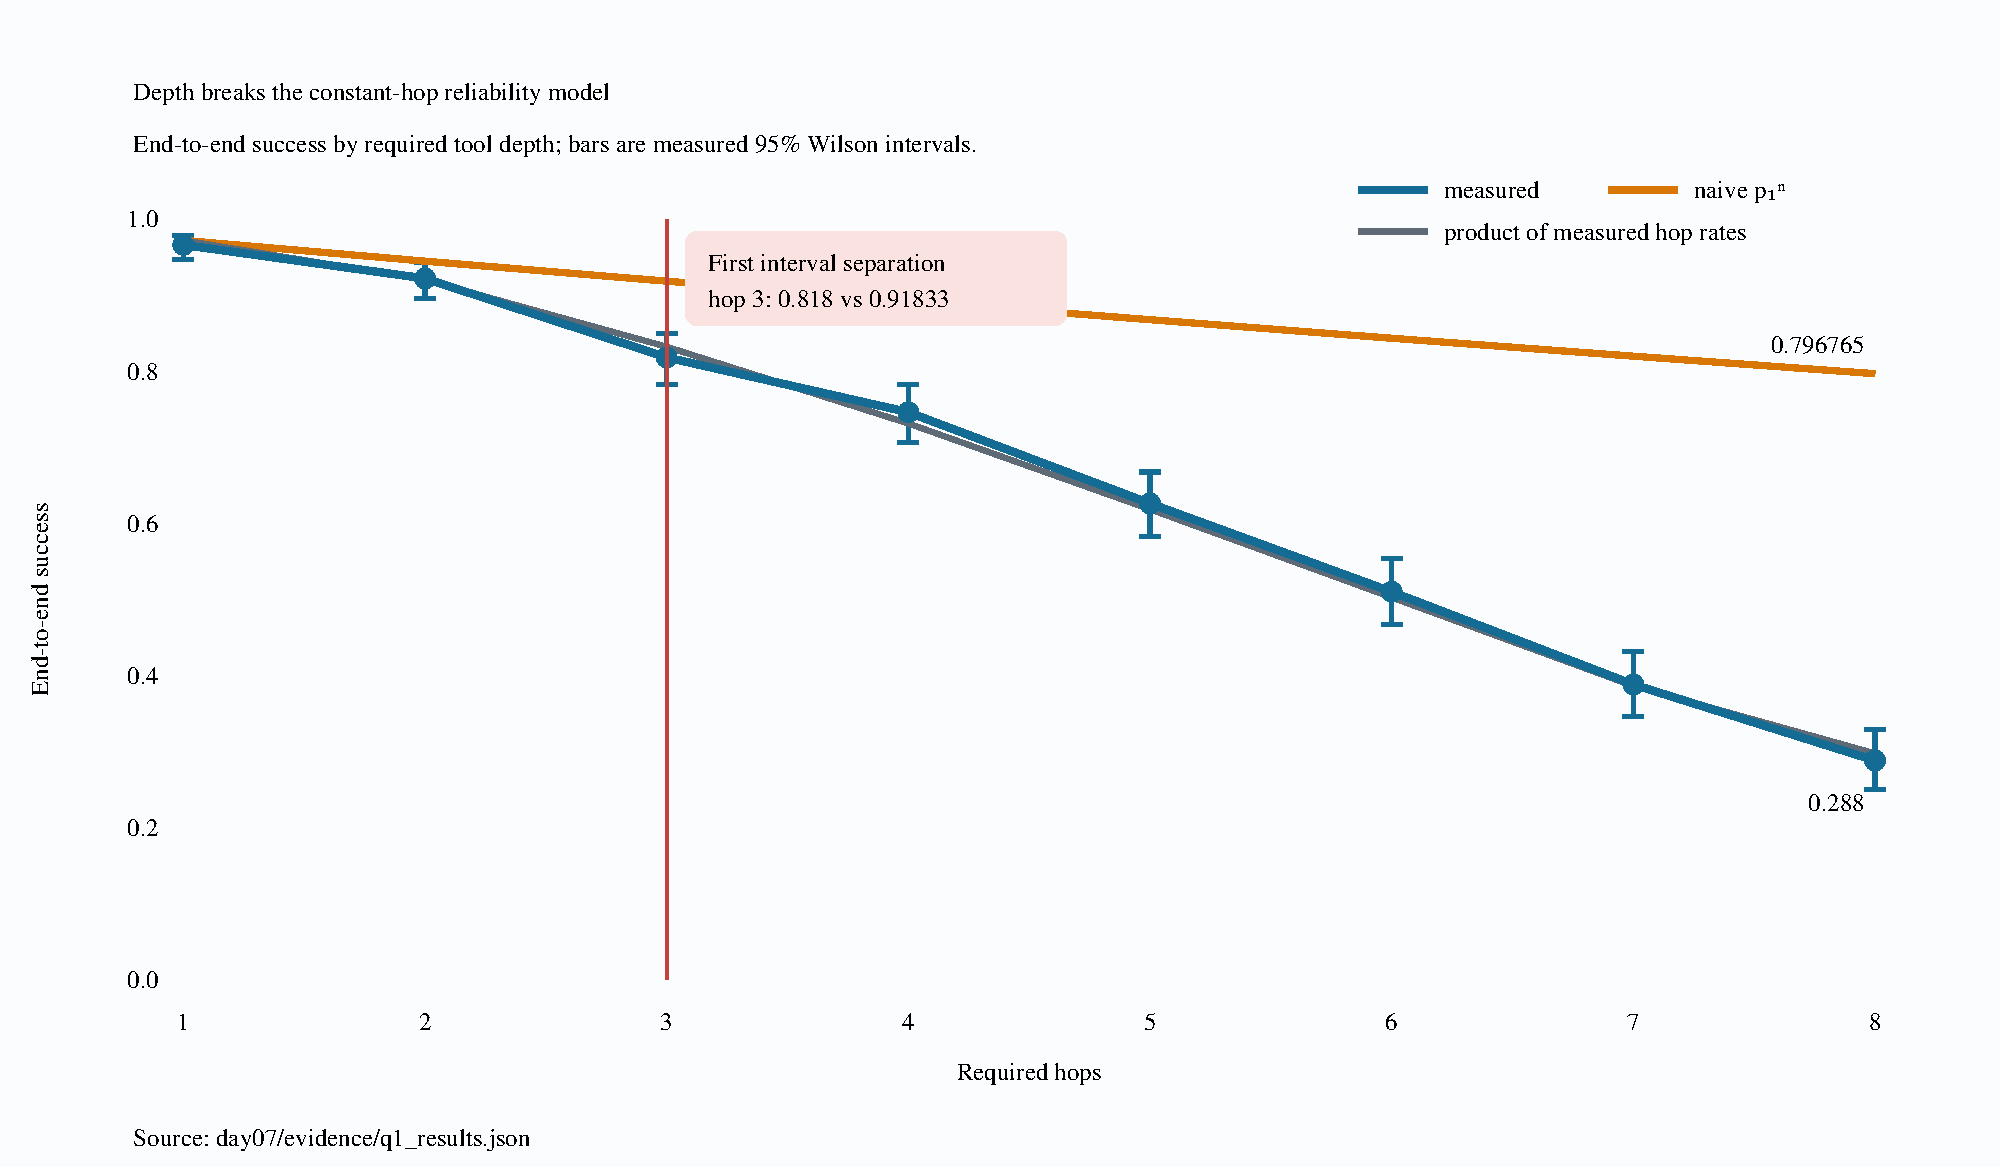
\includegraphics[width=0.72\textwidth,height=3.6cm,keepaspectratio,trim=7.4bp 3.6bp 52.0bp 32.4bp,clip]{fig1_depth.pdf}
\vspace{2pt}
\captionof{figure}{Measured vs Naive Multi-Hop Reliability by Required Tool Depth. The measured curve diverges from the naive $p_1^n$ model at depth 3, collapsing to $0.288$ at 8 hops versus $0.797$ predicted.}
\label{fig:q1_depth}
\end{center}

\begingroup
\small
\begin{itemize}\setlength{\itemsep}{1.2pt}\setlength{\parsep}{0pt}\setlength{\parskip}{0pt}
    \item \textbf{Question:} Does multi-step agent reliability follow a simple compounding of single-step accuracy ($P(\text{task}) = p_1^n$), or does the conditional probability change across sequential hops?
    \item \textbf{Hypothesis:} As required tool depth increases, conditional step difficulty increases due to accumulated context noise and error propagation; the measured curve will diverge from $p_1^n$ with disjoint confidence intervals.
    \item \textbf{Setup:} Seeded environment (\code{seed=42}); tool execution simulator with controlled noise; fixed agent reason-tool-observe loop.
    \item \textbf{Treatment:} Number of required tool hops varied systematically from $n=1$ to $n=8$.
    \item \textbf{Population:} 500 seeded trials per depth ($4,000$ total trials).
    \item \textbf{Metrics:} Single-hop reliability $p_1$, measured end-to-end task success $P(n)$, 95\% Wilson confidence intervals, naive prediction $p_1^n$.
    \item \textbf{Result:} \MEASURED
    \begin{itemize}\setlength{\itemsep}{0.8pt}\setlength{\parsep}{0pt}
        \item Single-hop base success: $p_1 = \mathbf{0.972}$.
        \item At 3 hops: Measured success was $\mathbf{0.818}$ (95\% CI: $[0.7818, 0.8494]$) vs naive prediction $\mathbf{0.91833}$. \textbf{First interval separation occurs at 3 hops}.
        \item At 8 hops: Measured success collapsed to $\mathbf{0.288}$ (95\% CI: $[0.2500, 0.3292]$) vs naive prediction $\mathbf{0.796765}$.
    \end{itemize}
    \item \textbf{Uncertainty:} The 95\% Wilson intervals strictly exclude the naive prediction for all depths $n \ge 3$.
    \item \textbf{Interpretation:} Tool hops are non-exchangeable. Error propagation and context accumulation degrade conditional success at later hops ($P(\text{step } k \mid \text{steps } 1 \dots k-1) < p_1$).
    \item \textbf{What it does NOT prove:} \LIMITATION\ (L02) It does not prove that every production LLM exhibits identical decay rates; it proves that planning assuming $p^n$ is mathematically invalid.
    \item \textbf{Reversal Condition:} Reverse if production multi-hop workloads show constant conditional success rates across deep traversal chains.
\end{itemize}
\endgroup

% ------------------------------------------------------------------------------
\subsection{Q2: Does an Aggregate Detector Score Conceal Operational Risk?}

\begin{center}
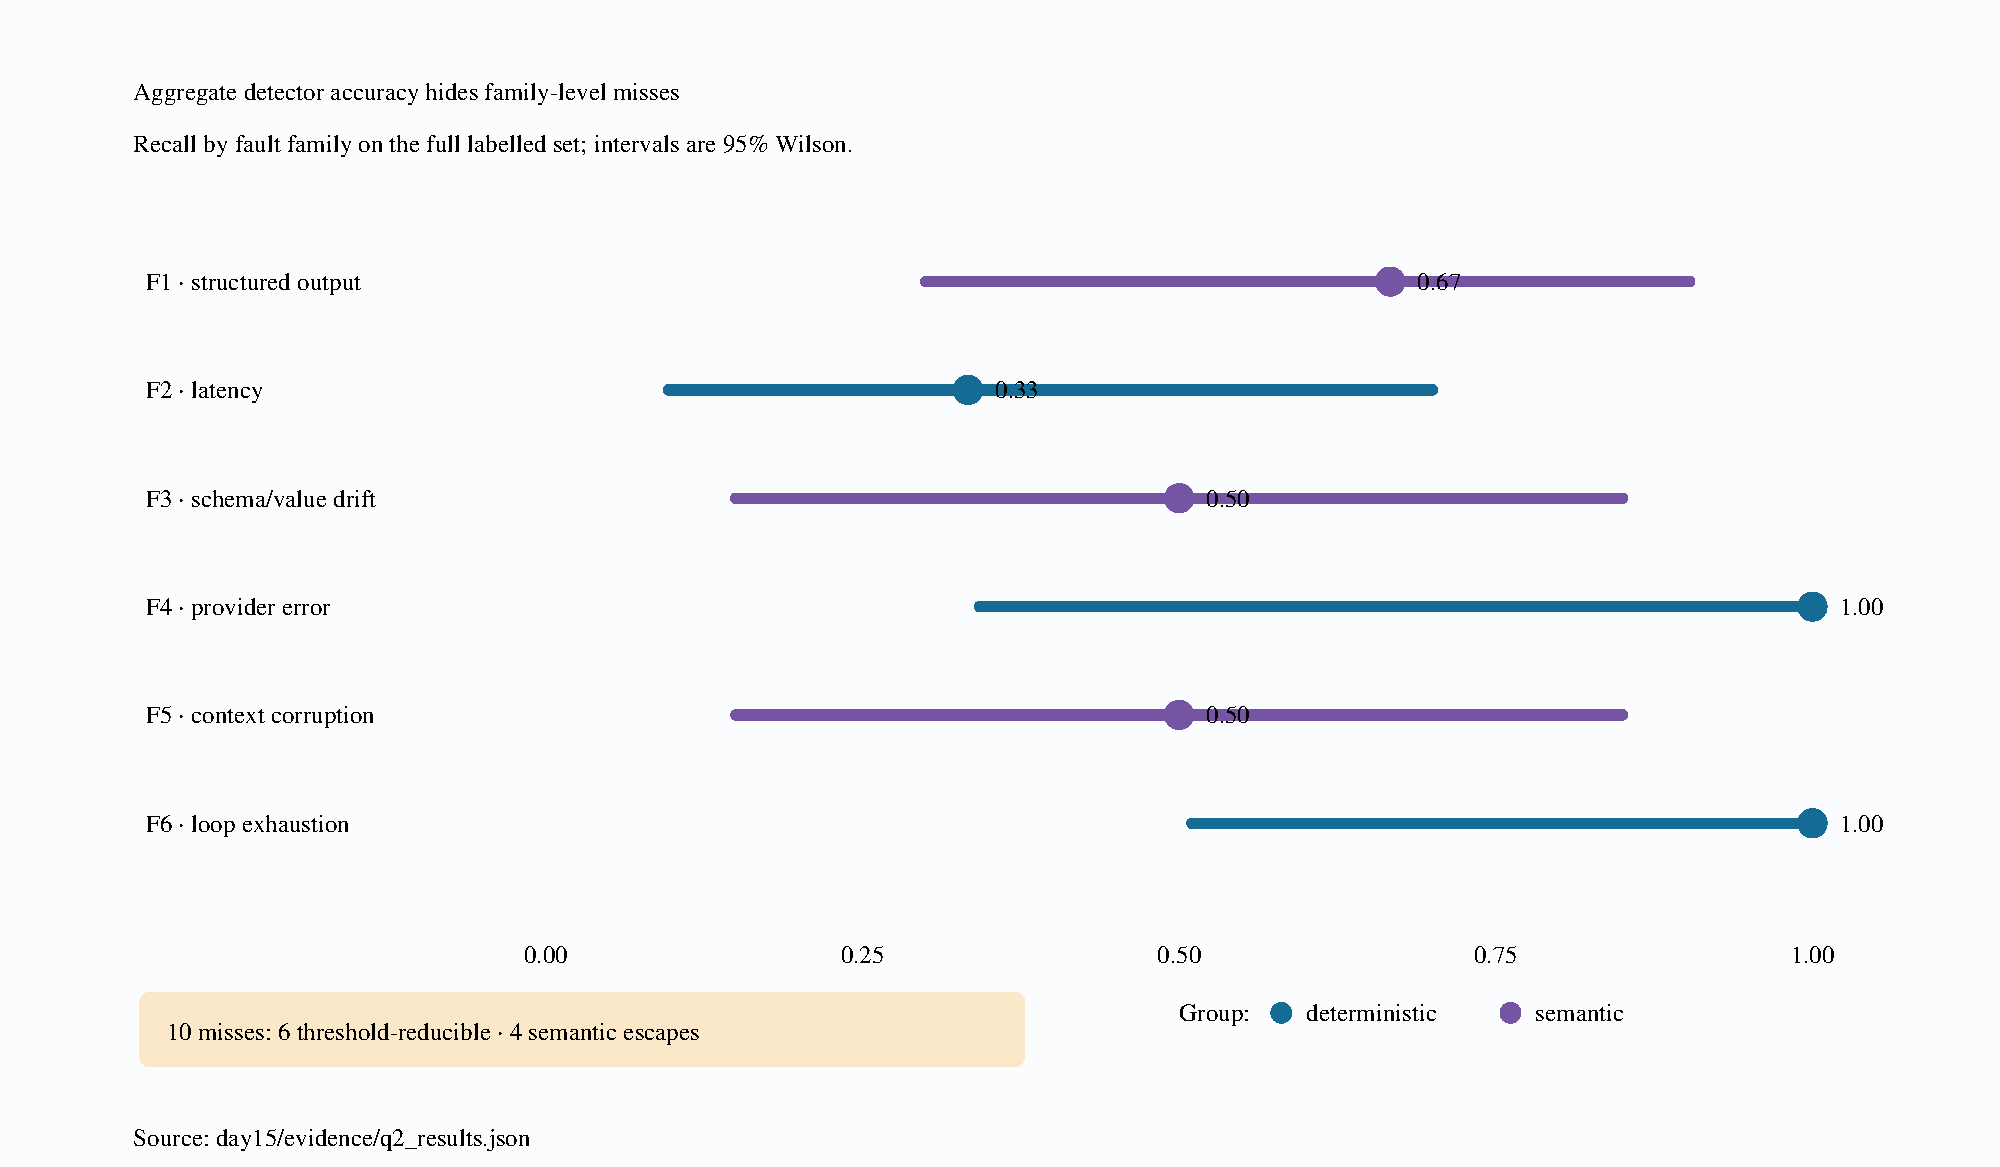
\includegraphics[width=0.72\textwidth,height=3.8cm,keepaspectratio,trim=61.0bp 3.6bp 53.0bp 32.4bp,clip]{fig2_detector.pdf}
\vspace{2pt}
\captionof{figure}{Detector Recall and Confidence Intervals by Fault Family. While aggregate precision was 1.0, micro recall was 0.615, concealing 10 false negatives (4 semantic escapes).}
\label{fig:q2_detector}
\end{center}

\begingroup
\small
\begin{itemize}\setlength{\itemsep}{1.2pt}\setlength{\parsep}{0pt}\setlength{\parskip}{0pt}
    \item \textbf{Question:} Can high aggregate detector metrics (e.g., F1 $>0.75$) conceal systemic failure modes that escape into user-visible answers?
    \item \textbf{Hypothesis:} Deterministic schema and latency detectors will achieve near-perfect recall on transport/syntax faults but completely fail on semantic corruption.
    \item \textbf{Setup:} 44 human-labelled traces covering fault families F1--F6 across severities 1 to 3; out-of-band injection truth.
    \item \textbf{Treatment:} Application of deterministic multi-fault detector vs injection ground truth.
    \item \textbf{Population:} 44 labelled test runs.
    \item \textbf{Metrics:} Micro/Macro Precision, Recall, F1 score, confusion matrices, miss audit.
    \item \textbf{Result:} \MEASURED
    \begin{itemize}\setlength{\itemsep}{0.8pt}\setlength{\parsep}{0pt}
        \item Precision: $\mathbf{1.000}$ (Zero false alarms).
        \item Recall: $\mathbf{0.615385}$ (10 false negatives out of 26 faulted cases).
        \item Aggregate F1: $\mathbf{0.761905}$.
        \item Miss Audit: 6 misses were threshold-reducible; \textbf{4 were semantic escapes} (F3 wrong data, F5 context drift).
    \end{itemize}
    \item \textbf{Uncertainty:} Wilson intervals on per-fault recall are wide due to small sample slices ($n=44$).
    \item \textbf{Interpretation:} High aggregate scores create false security. Evaluators must audit the miss mechanism. Deterministic checks cannot catch subtle semantic corruptions.
    \item \textbf{What it does NOT prove:} \LIMITATION\ (L03) Does not prove that semantic detectors are impossible; proves deterministic checks require semantic guards.
    \item \textbf{Reversal Condition:} Reverse if a single unified detector demonstrates $\ge 0.95$ recall across both transport and semantic miss slices.
\end{itemize}
\endgroup

% ------------------------------------------------------------------------------
\subsection{Q3: Is a Retry Cap Stable Across Fault Structure (Correlation)?}

\begin{center}
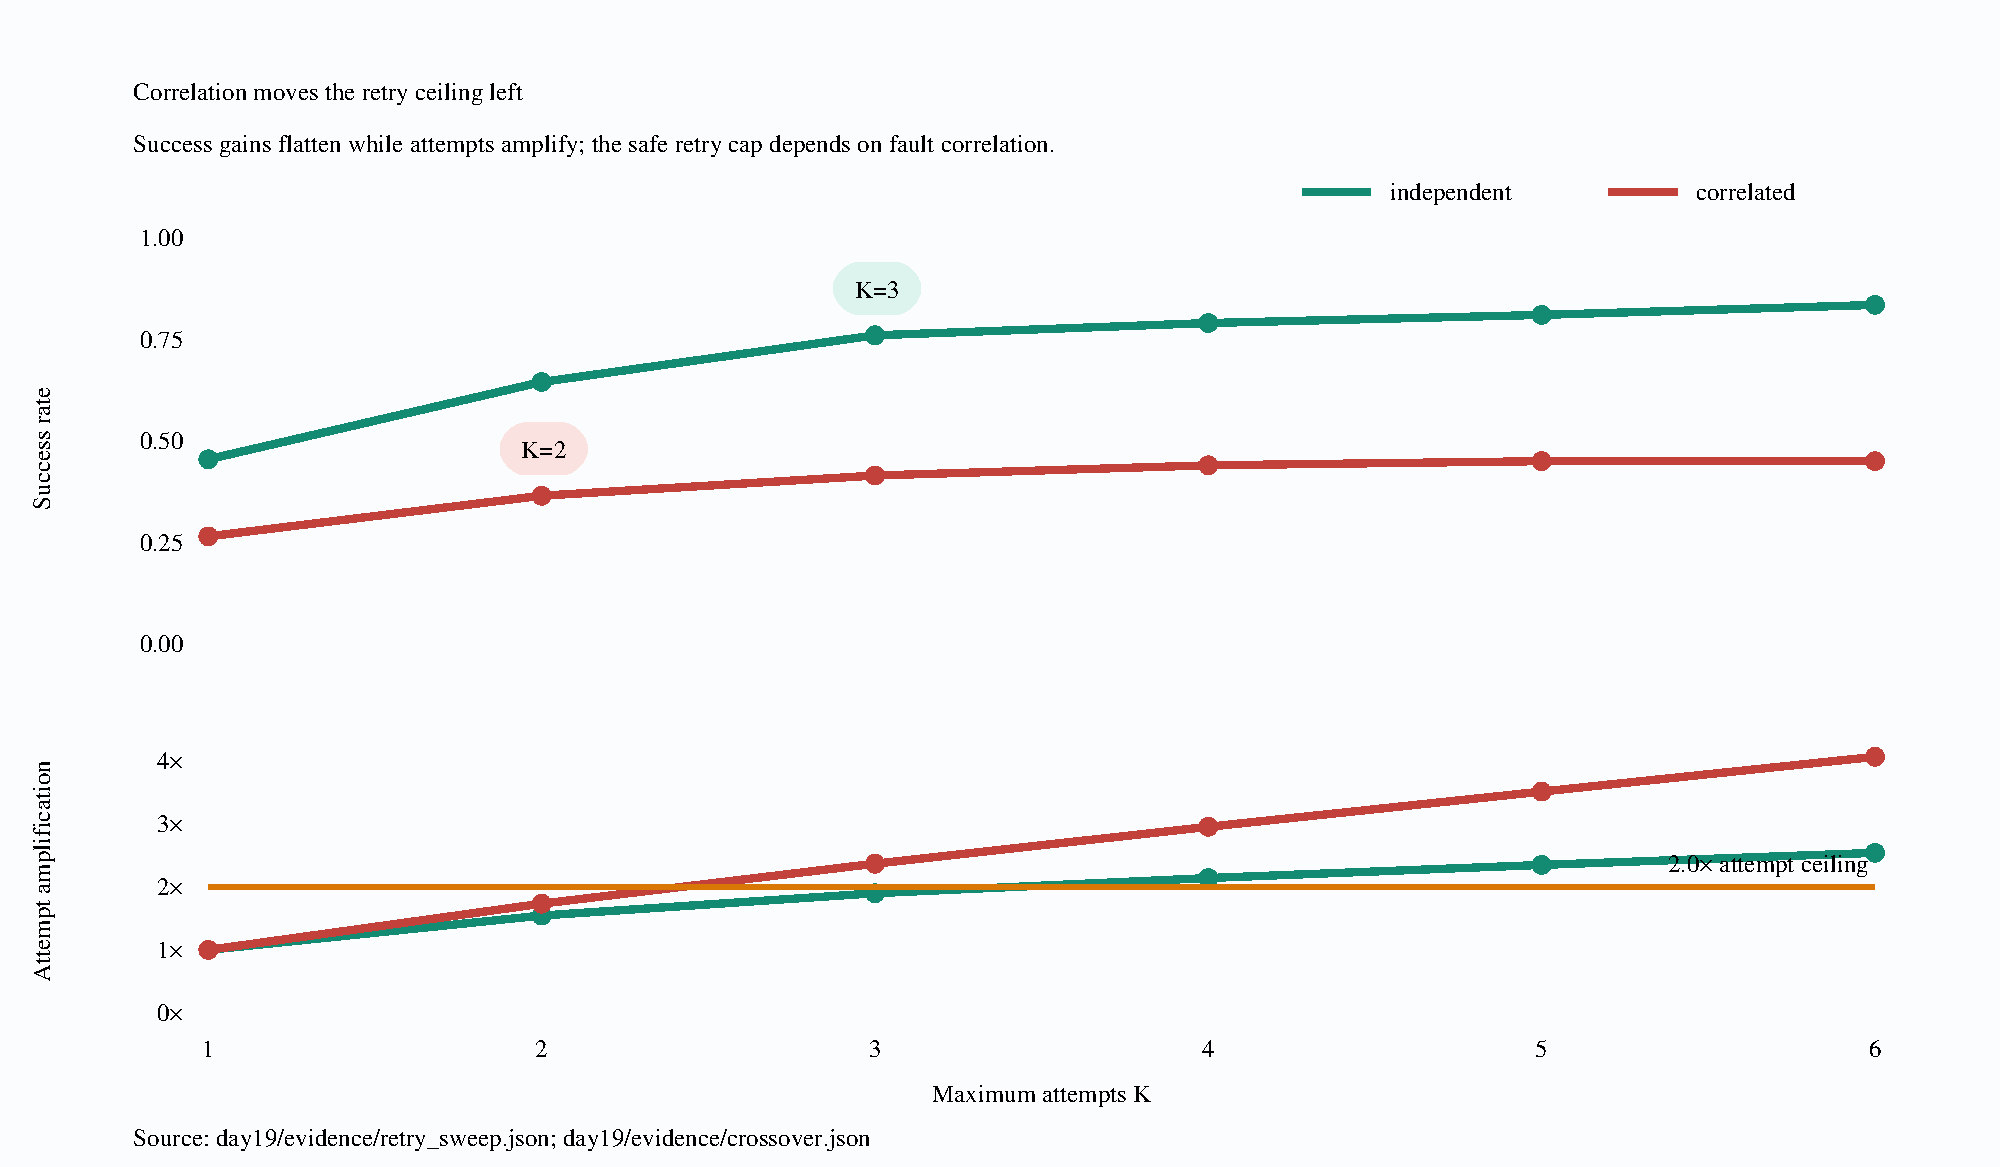
\includegraphics[width=0.72\textwidth,height=3.8cm,keepaspectratio,trim=8.4bp 3.6bp 52.5bp 32.4bp,clip]{fig3_retry.pdf}
\vspace{2pt}
\captionof{figure}{Success Rate and Attempt Amplification by Retry Cap ($K$) Under Independent vs Correlated Faults. During correlated outages, $K=3$ amplifies load to $2.37\times$ while buying negligible success.}
\label{fig:q3_retry}
\end{center}

\begingroup
\small
\begin{itemize}\setlength{\itemsep}{1.2pt}\setlength{\parsep}{0pt}\setlength{\parskip}{0pt}
    \item \textbf{Question:} Does the optimal retry budget ($K$) determined under independent transient faults remain optimal during correlated provider outages?
    \item \textbf{Hypothesis:} When failures are correlated, retries fail repeatedly, amplifying system load and breaching latency ceilings without improving success.
    \item \textbf{Setup:} 200 shared scenario seeds; virtual latency model; decision ceilings of $2.0\times$ attempt amplification and $120$ latency units.
    \item \textbf{Treatment:} Varying retry cap $K \in \{0, 1, 2, 3, 4, 5\}$ under independent vs correlated failure regimes.
    \item \textbf{Population:} 200 paired requests per sweep point ($2,400$ total executions).
    \item \textbf{Metrics:} Task success, attempt amplification factor, p99 tail latency, McNemar paired p-value.
    \item \textbf{Result:} \MEASURED
    \begin{itemize}\setlength{\itemsep}{0.8pt}\setlength{\parsep}{0pt}
        \item Under independent faults: Optimal cap inside budget ceilings was $\mathbf{K=3}$ (Success $\mathbf{0.760}$, Amplification $\mathbf{1.90\times}$, p99 latency $\mathbf{76.0}$).
        \item Under correlated faults: Optimal cap inside budget ceilings dropped to $\mathbf{K=2}$ (Success $\mathbf{0.365}$, Amplification $\mathbf{1.735\times}$, p99 latency $\mathbf{53.4}$).
        \item Setting $K=3$ under correlation caused attempt amplification to spike to $\mathbf{2.37\times}$ (breaching the $2.0\times$ ceiling) for only $\mathbf{0.415}$ success.
        \item McNemar paired test comparing independent vs correlated success at $K=3$: $p = \mathbf{2.695 \times 10^{-16}}$.
    \end{itemize}
    \item \textbf{Uncertainty:} Highly significant paired difference ($p \ll 10^{-6}$) over identical seeds.
    \item \textbf{Interpretation:} Correlation changes the operational boundary. During an outage, retrying the same dependency amplifies the outage (a retry storm).
    \item \textbf{What it does NOT prove:} \LIMITATION\ (L05) The exact crossover point ($K=2$ vs $K=3$) is a function of the configured simulator parameters.
    \item \textbf{Reversal Condition:} Reverse if provider endpoints exhibit zero failure correlation under heavy burst load.
\end{itemize}
\endgroup

% ------------------------------------------------------------------------------
\subsection{Q4: Does Fallback Preserve Availability Without Preserving Quality?}

\begin{center}
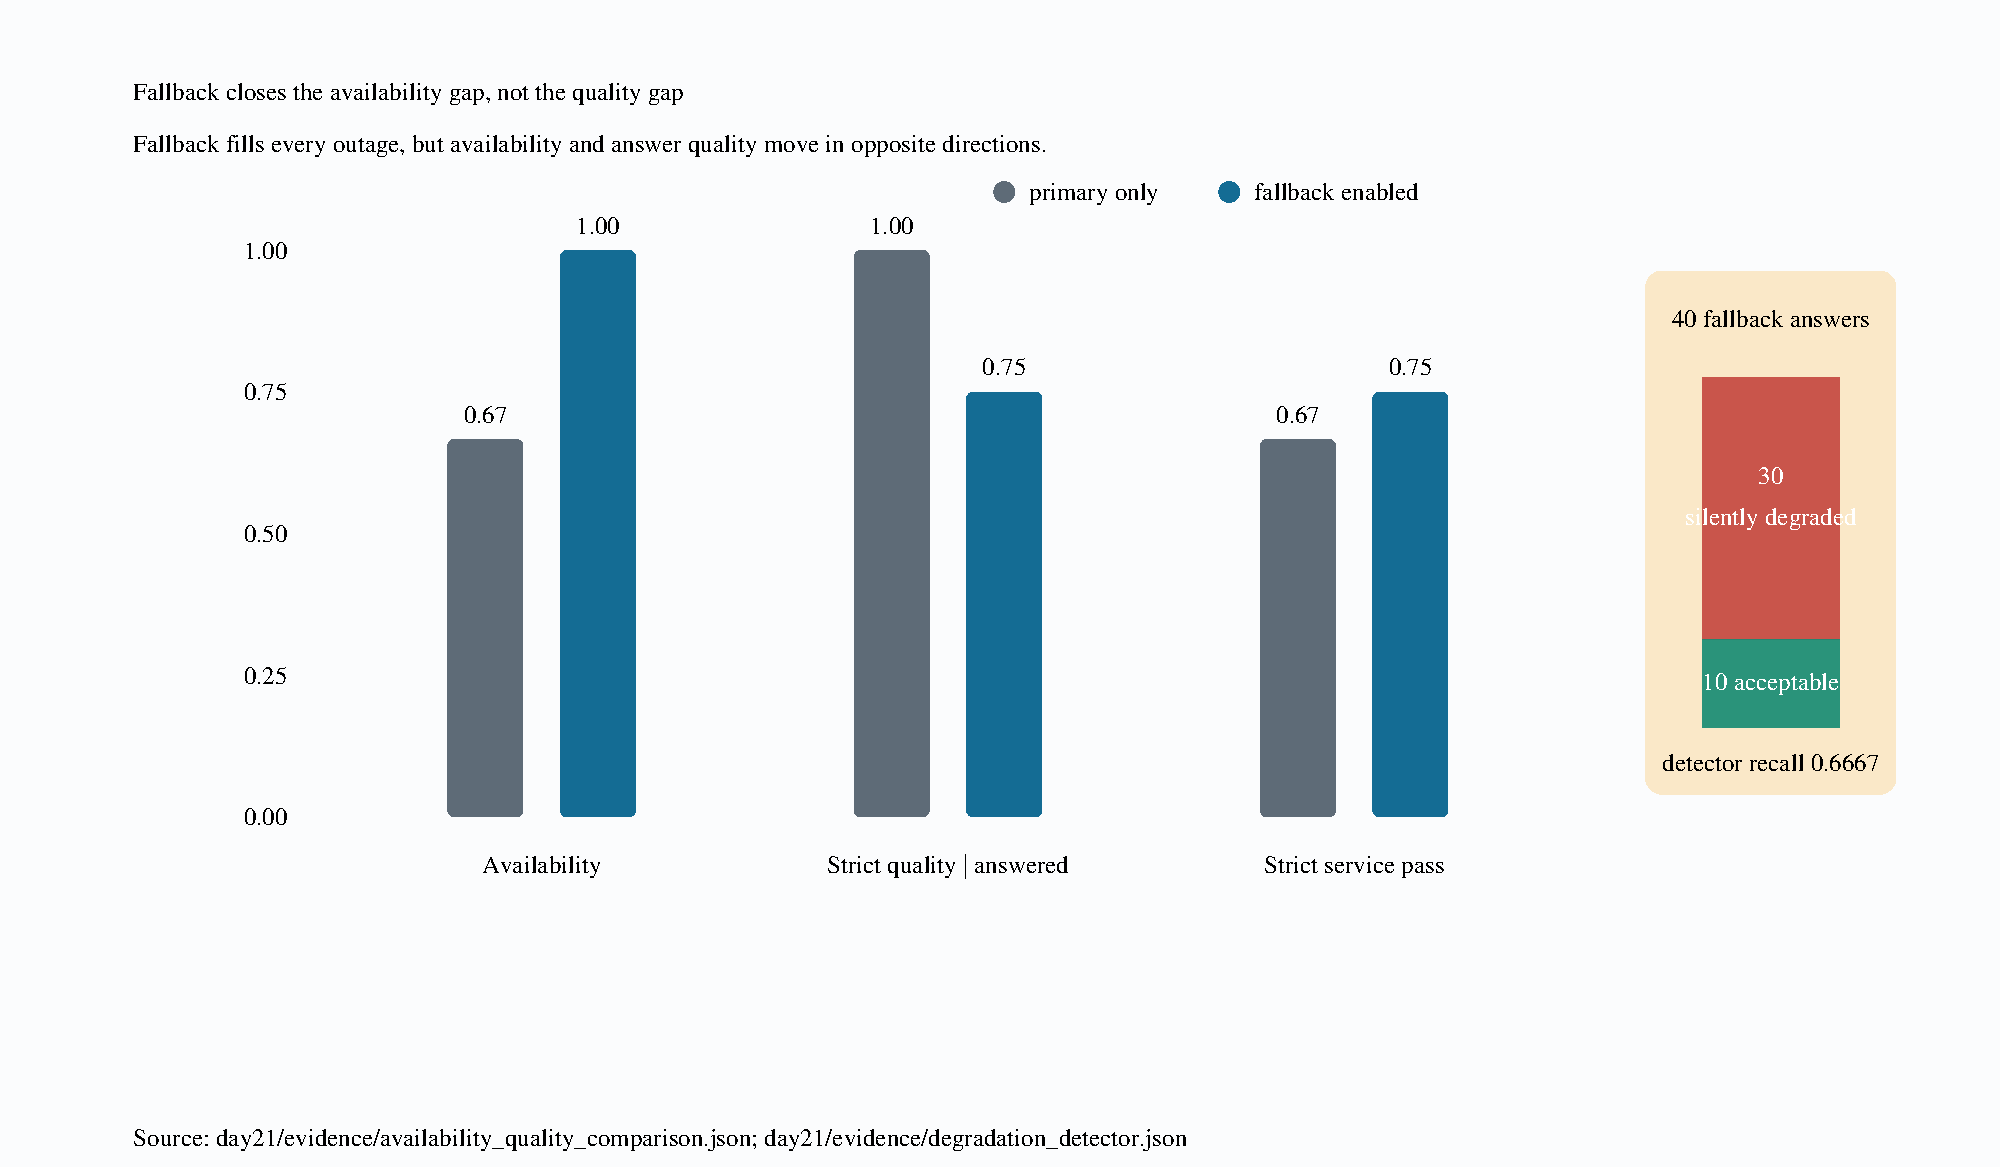
\includegraphics[width=0.72\textwidth,height=3.8cm,keepaspectratio,trim=61.0bp 3.6bp 47.0bp 32.4bp,clip]{fig4_fallback.pdf}
\vspace{2pt}
\captionof{figure}{Availability vs Strict Quality Under Primary Provider Outage. Fallback restores availability from 0.667 to 1.0, but strict answer quality drops from 1.0 to 0.75 (30 of 40 fallback answers degraded).}
\label{fig:q4_fallback}
\end{center}

\begingroup
\small
\begin{itemize}\setlength{\itemsep}{1.2pt}\setlength{\parsep}{0pt}\setlength{\parskip}{0pt}
    \item \textbf{Question:} Does automated fallback to a secondary model preserve service availability at the expense of returning degraded, inaccurate answers?
    \item \textbf{Hypothesis:} Fallback will achieve 100\% availability on the transport layer while significantly reducing strict semantic answer quality.
    \item \textbf{Setup:} 120 paired requests; 40 scheduled primary provider outages; fallback to a cheaper, faster secondary model; strict programmatic oracle.
    \item \textbf{Treatment:} Primary-only routing vs Automated secondary fallback routing.
    \item \textbf{Population:} 120 paired requests.
    \item \textbf{Metrics:} Service availability, strict answer quality given answered, overall service pass rate, fallback answer degradation rate.
    \item \textbf{Result:} \MEASURED
    \begin{itemize}\setlength{\itemsep}{0.8pt}\setlength{\parsep}{0pt}
        \item Primary-only baseline: Availability was $\mathbf{0.6667}$ ($80/120$); strict answer quality among answered was $\mathbf{1.000}$ ($80/80$). Overall pass: $\mathbf{0.6667}$.
        \item Fallback-enabled: Availability rose to $\mathbf{1.000}$ ($120/120$); strict answer quality plunged to $\mathbf{0.7500}$ ($90/120$). Overall pass: $\mathbf{0.7500}$.
        \item Fallback slice decomposition: Of the 40 fallback answers, \textbf{30 were silently degraded} (75\% degradation rate).
        \item Advisory detector recall on degraded answers was only $\mathbf{0.6667}$ ($20/30$), missing all 10 borderline-token corruptions.
    \end{itemize}
    \item \textbf{Uncertainty:} 95\% Wilson interval on fallback degradation is $[0.598, 0.858]$.
    \item \textbf{Interpretation:} Fallback trades correctness for availability. A dashboard showing 100\% uptime is actively misleading when 25\% of all served answers are wrong.
    \item \textbf{What it does NOT prove:} \LIMITATION\ (L06) The $75\%$ degradation rate reflects the configured capability gap between the primary and fallback models.
    \item \textbf{Reversal Condition:} Reverse if the fallback model possesses identical reasoning capability and knowledge cutoff as the primary model.
\end{itemize}
\endgroup

% ------------------------------------------------------------------------------
\subsection{Q5: Which Recovery Policy Wins on Correct Success, Cost, and Latency?}

\begin{center}
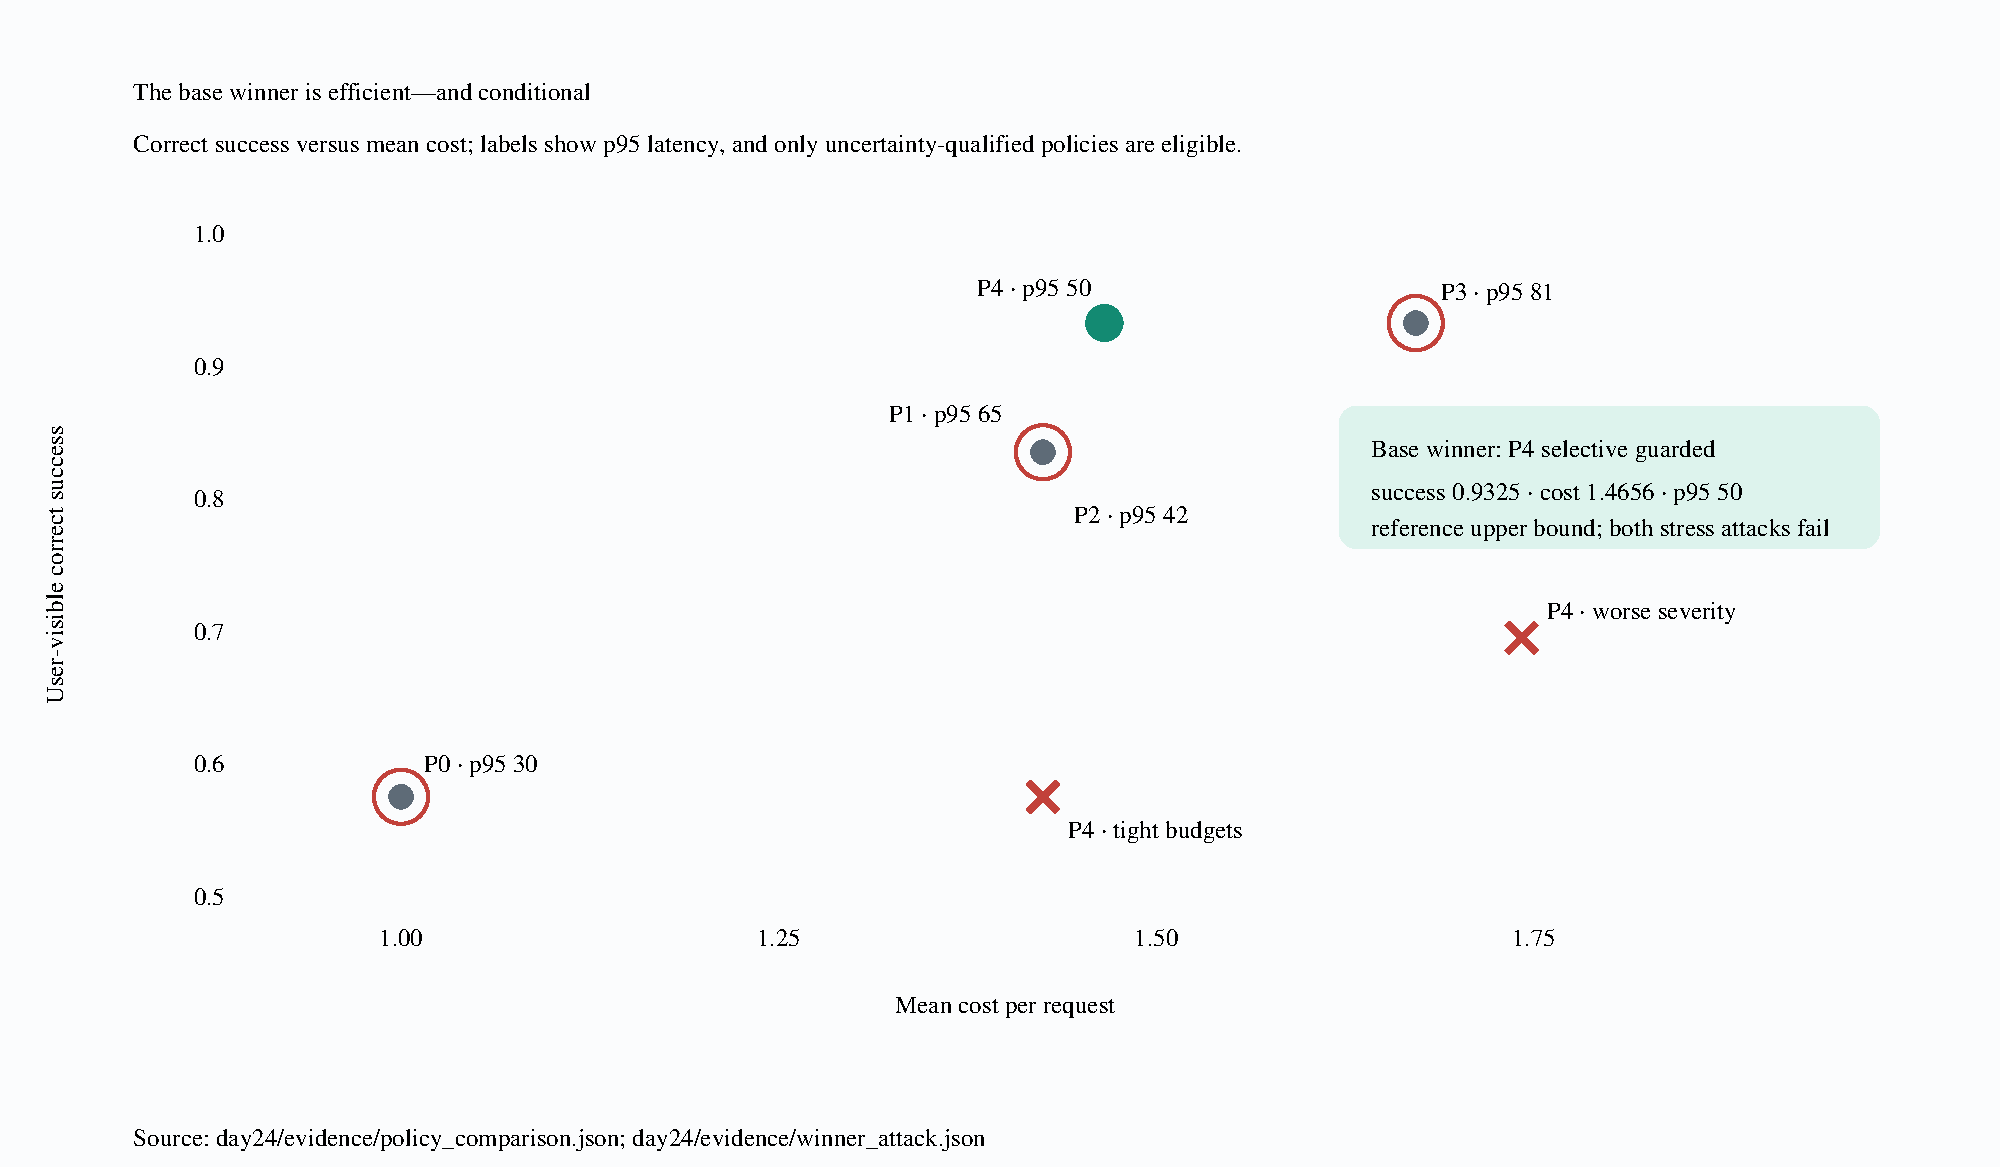
\includegraphics[width=0.72\textwidth,height=3.8cm,keepaspectratio,trim=14.4bp 3.6bp 55.0bp 32.4bp,clip]{fig5_policy.pdf}
\vspace{2pt}
\captionof{figure}{Policy Pareto Frontier: Correct Success vs Mean Cost across 400 Shared Seeds. P4 Selective Guarded is the base-envelope winner, but collapses under stress attacks.}
\label{fig:q5_policy}
\end{center}

\begingroup
\small
\begin{itemize}\setlength{\itemsep}{1.2pt}\setlength{\parsep}{0pt}\setlength{\parskip}{0pt}
    \item \textbf{Question:} Which recovery cascade policy delivers the highest user-visible correct success within strict cost and tail-latency constraints?
    \item \textbf{Hypothesis:} A selective guarded policy that retries only transient faults and gates fallback on answer quality will dominate naive retry and blind fallback.
    \item \textbf{Setup:} 400 shared seeds ($2026080300 \dots 2026080699$); five candidate policies (P0--P4); constraint-first eligibility screen: Success lower bound $\ge 0.78$, Wrong-answer upper bound $\le 0.02$, Mean cost $\le 1.75$, p95 latency $\le 80$.
    \item \textbf{Treatment:} P0 (No recovery), P1 (Bounded retry), P2 (Unchecked fallback), P3 (Full cascade), P4 (Selective guarded).
    \item \textbf{Population:} 400 paired requests.
    \item \textbf{Metrics:} Correct success, wrong visible answers, mean cost, p95 latency, efficiency ratios.
    \item \textbf{Result:} \MEASURED
    \begin{itemize}\setlength{\itemsep}{0.8pt}\setlength{\parsep}{0pt}
        \item P0: Success $0.5750$ (Fails success floor).
        \item P2: Success $0.8350$, Wrong answers $\mathbf{0.1650}$ (Fails wrong-answer bound $\le 0.02$).
        \item P3: Success $0.9325$, Mean cost $1.6719$, p95 latency $\mathbf{81.0}$ (Fails latency bound $\le 80$).
        \item \textbf{P4 Selective Guarded (WINNER):} Correct success $\mathbf{0.9325}$ (95\% CI: $[0.9036, 0.9532]$); Wrong answers $\mathbf{0}$ (Wilson upper bound $\mathbf{0.0095}$); Mean cost $\mathbf{1.4656}$ (Bootstrap 95\% CI: $[1.410, 1.521]$); p95 latency $\mathbf{50.0}$.
        \item Paired delta vs P1: $+0.0950$ success ($p = 1.95 \times 10^{-9}$); $+0.0485$ success/cost ($[0.0319, 0.0664]$).
        \item \textbf{Stress Attacks on Winner:} Under worse severity, P4 success dropped to $\mathbf{0.6950}$ (failed); under tight budgets, success dropped to $\mathbf{0.5750}$ (failed).
    \end{itemize}
    \item \textbf{Uncertainty:} Paired bootstrap intervals strictly exceed zero against all eligible competitors in baseline conditions.
    \item \textbf{Interpretation:} P4 is the reference upper bound in the measured base envelope. Its failure under stress proves that no policy can be deployed without runtime envelope monitoring.
    \item \textbf{What it does NOT prove:} \LIMITATION\ (L07) P4 received an idealized retryability classifier; real-world classifier noise will lower this upper bound.
    \item \textbf{Reversal Condition:} Reverse if production error classification has $<70\%$ accuracy or if fallback quality cannot be verified at runtime.
\end{itemize}
\endgroup

\clearpage
\section{The 30-Day Engineering Journey}

The 30-day progression was executed in four disciplined phases:

\begin{center}
\resizebox{0.98\textwidth}{!}{%
\begin{tikzpicture}[
  node distance=0.4cm,
  phasebox/.style={draw=primary, fill=white, rounded corners=3pt, font=\footnotesize\sffamily, align=center, inner sep=5pt, line width=0.8pt, minimum height=1.3cm},
  arrow/.style={-{Latex[length=2.5mm]}, line width=1.2pt, color=primary}
]
\node[phasebox, fill=blue!5] (pa) {\textbf{Phase A: Days 01--07}\\Measurement Foundations\\{\scriptsize Seeded World $\cdot$ Oracle $\cdot$ Tracing $\cdot$ Q1}};
\node[phasebox, fill=teal!5, right=of pa] (pb) {\textbf{Phase B: Days 08--17}\\Statistical \& Causal Discipline\\{\scriptsize Faults F1--F6 $\cdot$ Detectors $\cdot$ Q2 $\cdot$ Judge}};
\node[phasebox, fill=warning!5, right=of pb] (pc) {\textbf{Phase C: Days 18--25}\\Operational Recovery\\{\scriptsize Retries $\cdot$ Breakers $\cdot$ Fallback $\cdot$ Q3--Q5}};
\node[phasebox, fill=success!5, right=of pc] (pd) {\textbf{Phase D: Days 26--30}\\Evidence Operations\\{\scriptsize Docker $\cdot$ Cold Repro $\cdot$ Audit $\cdot$ Defense}};

\draw[arrow] (pa) -- (pb);
\draw[arrow] (pb) -- (pc);
\draw[arrow] (pc) -- (pd);
\end{tikzpicture}%
}
\end{center}

\begin{center}
\scriptsize
\begin{longtable}{l>{\raggedright\arraybackslash}p{0.20\textwidth}>{\raggedright\arraybackslash}p{0.25\textwidth}>{\raggedright\arraybackslash}p{0.25\textwidth}l}
\toprule
\textbf{Day} & \textbf{Core Objective} & \textbf{Engineering Deliverable} & \textbf{Key Learning / Finding} & \textbf{Status} \\
\midrule
\endfirsthead
\toprule
\textbf{Day} & \textbf{Core Objective} & \textbf{Engineering Deliverable} & \textbf{Key Learning / Finding} & \textbf{Status} \\
\midrule
\endhead
\midrule
\multicolumn{5}{r}{\textit{Continued on next page\dots}} \\
\bottomrule
\endfoot
\bottomrule
\endlastfoot

\textbf{01} & Pure-function ground truth & \code{day01/oracle.py}; exact answer token check & Deterministic oracle must exist before agent code is written. & \STATUSVALIDATED \\
\textbf{02} & Seeded document corpus & 300 entities, 60 distractors, 350 scenarios & Eliminating environmental drift isolates agent behavior. & \STATUSVALIDATED \\
\textbf{03} & Bounded ReAct agent loop & Reason $\to$ Tool $\to$ Observe loop with step cap & Multi-step loops require hard terminating invariants. & \STATUSVALIDATED \\
\textbf{04} & Pydantic tool contracts & Typed contracts for \code{search}, \code{lookup}, \code{calc} & \code{extra="forbid"} catches schema drift immediately. & \STATUSVALIDATED \\
\textbf{05} & SQLite persistent traces & Crash-surviving execution span storage & Memory logs are lost during OOM crashes; SQLite survives. & \STATUSVALIDATED \\
\textbf{06} & Single-step accuracy baseline & Single-hop retrieval benchmark ($p_1 = 0.972$) & High single-step accuracy creates false confidence. & \STATUSVALIDATED \\
\textbf{07} & Multi-hop depth benchmark (Q1) & 4,000 runs across depths $1 \dots 8$; Wilson CIs & \textbf{Failure compounding: $P(n) < p_1^n$ starting at hop 3.} & \STATUSVALIDATED \\
\midrule
\textbf{08} & Failure taxonomy (F1--F6) & Physical fault catalog across component boundaries & Failures must be classified by producing component. & \STATUSVALIDATED \\
\textbf{09} & Deterministic fault injector & Transport \& data fault injection proxy & Ground truth must be logged out-of-band to prevent leakage. & \STATUSVALIDATED \\
\textbf{10} & Latency \& timeout modeling & Virtual time simulation for network delays & Latency distribution is heavily multimodal during outages. & \STATUSVALIDATED \\
\textbf{11} & Semantic drift injection & Distractor poisoning \& attribute mismatch & Valid syntax can carry totally invalid semantic tokens. & \STATUSVALIDATED \\
\textbf{12} & Catalog test gallery & Comprehensive test suite for injectors & Injector must be verified independent of the agent. & \STATUSVALIDATED \\
\textbf{13} & Deterministic failure detectors & Rule-based syntax \& latency anomaly checks & Deterministic checks achieve 1.0 precision on transport faults. & \STATUSVALIDATED \\
\textbf{14} & Statistical verification suite & Wilson, McNemar, and Bootstrap library & Paired tests over identical seeds eliminate query variance. & \STATUSVALIDATED \\
\textbf{15} & Detector benchmark (Q2) & 44 labelled traces; Precision/Recall audit & \textbf{Vanity F1 (0.76) concealed 10 false negatives (4 semantic).} & \STATUSVALIDATED \\
\textbf{16} & LLM-as-a-judge validation & Cohen's kappa evaluation on human golden set & \textbf{Judge failed ($\kappa = 0.50$); quarantined to advisory status.} & \STATUSVALIDATED \\
\textbf{17} & Mid-point architecture review & Consolidation of Phase 1 evidence & Without programmatic gates, reliability metrics drift. & \STATUSVALIDATED \\
\midrule
\textbf{18} & Recovery primitives (M1--M6) & Bounded retry, timeout, circuit breaker & Recovery mechanisms alter downstream probability distributions. & \STATUSVALIDATED \\
\textbf{19} & Retry crossover sweep (Q3) & 2,400 runs across $K \in \{0 \dots 5\}$; paired tests & \textbf{Optimal retry drops from $K=3$ to $K=2$ under correlation.} & \STATUSVALIDATED \\
\textbf{20} & Circuit breaker implementation & Three-state rolling window breaker & Fast-failing during outages prevents cascading storms. & \STATUSVALIDATED \\
\textbf{21} & Fallback quality benchmark (Q4) & 120 paired runs; primary vs secondary fallback & \textbf{Availability rose to 1.0; quality collapsed to 0.75.} & \STATUSVALIDATED \\
\textbf{22} & 36-cell recovery matrix & Full evaluation across 6 mechanisms $\times$ 6 faults & \textbf{Discovered 47 induced harms from automated recovery.} & \STATUSVALIDATED \\
\textbf{23} & Adaptive recovery cascade & Multi-objective policy routing (P0--P4) & Constraint-first screening beats scalar score optimization. & \STATUSVALIDATED \\
\textbf{24} & Policy Pareto optimization (Q5) & 400 shared seeds; frontier analysis & \textbf{P4 Selective Guarded wins base; collapses under stress.} & \STATUSVALIDATED \\
\textbf{25} & Postmortem incident replay & Deterministic red $\to$ green regression suite & Production fixes must pass 20 consecutive runs on same seed. & \STATUSVALIDATED \\
\midrule
\textbf{26} & Self-explaining reproducibility & \code{readme\_claims.json}; \code{make reproduce} & Every README number bound to committed JSON pointer in CI. & \STATUSVALIDATED \\
\textbf{27} & Cold-reader reproduction gate & Pinned Docker image; public clone test & Stranger clones repo and reproduces headline results with 0 errors. & \STATUSVALIDATED \\
\textbf{28} & Publication bundle \& audit & \code{day28/ARTICLE.md}; \code{claim\_audit.py} & All 29 registered claims verified against source files and limits. & \STATUSVALIDATED \\
\textbf{29} & 3-minute demo \& case study & 2:45 terminal recording (\code{.cast}); case study & Narrative compression must preserve underlying proof boundaries. & \STATUSVALIDATED \\
\textbf{30} & Defense guide \& launch gate & 10 skeptical staff Q\&As; launch checklist & Reliability engineer must defend tradeoffs, limits, and reversals. & \STATUSVALIDATED \\
\end{longtable}
\end{center}

% ==============================================================================
\vspace{12pt}
\needspace{8\baselineskip}
\section{What Was Actually Built}

To separate completed engineering artifacts from speculative proposals, the table below catalogs all major repository components, their implementation location, operational status, and verification evidence:

\begin{center}
\begingroup
\small
\setlength{\tabcolsep}{3pt}
\renewcommand{\code}[1]{{\scriptsize\ttfamily\nolinkurl{#1}}}
\begin{longtable}{>{\raggedright\arraybackslash}p{0.20\textwidth}>{\raggedright\arraybackslash}p{0.22\textwidth}>{\raggedright\arraybackslash}p{0.14\textwidth}>{\raggedright\arraybackslash}p{0.21\textwidth}>{\raggedright\arraybackslash}p{0.17\textwidth}}
\toprule
\textbf{Component} & \textbf{System Purpose} & \textbf{Status} & \textbf{Committed Evidence} & \textbf{Repository Location} \\
\midrule
\endfirsthead
\toprule
\textbf{Component} & \textbf{System Purpose} & \textbf{Status} & \textbf{Committed Evidence} & \textbf{Repository Location} \\
\midrule
\endhead
\midrule
\multicolumn{5}{r}{\textit{Continued on next page\dots}} \\
\bottomrule
\endfoot
\bottomrule
\endlastfoot

\textbf{Deterministic Corpus} & Generates 1,164 docs, 350 scenarios with link layer & \STATUSVALIDATED & Content hash verified; max reuse $\le 5$ & \code{faultline_p2/env/corpus.py} \\
\addlinespace
\textbf{Pure-Function Oracle} & Evaluates exact answer token and required source IDs & \STATUSVALIDATED & Hash-pinned copy (\code{dc5eef...}); 0 drift & \code{faultline_p2/oracle/} \\
\addlinespace
\textbf{Bounded Agent Loop} & Executes reason-tool-observe; 12-step cap; typed tools & \STATUSVALIDATED & Tested across 350 scenarios in \code{test_x2} & \code{faultline_p2/agent/agent.py} \\
\addlinespace
\textbf{Tool Contracts} & Search (500-char snippet), Lookup (scoped), Calc & \STATUSVALIDATED & Pydantic v2 \code{extra="forbid"} & \code{faultline_p2/agent/tools.py} \\
\addlinespace
\textbf{Fault Injector} & Deterministic injection of F1--F6 with out-of-band truth & \STATUSVALIDATED & Catalog gallery and trace tests & \code{day12/faultline_catalog/} \\
\addlinespace
\textbf{SQLite Trace Store} & Crash-surviving span storage with foreign keys & \STATUSVALIDATED & \code{trace.db} schema tests & \code{faultline_p2/trace/store.py} \\
\addlinespace
\textbf{OTel GenAI Exporter} & Emits traces to SemConv v1.29.0 OTLP JSON & \STATUSVALIDATED & 100\% schema match; 0 drift (P02) & \code{faultline_p2/otel/exporter.py} \\
\addlinespace
\textbf{SRE Alert Evaluator} & Multi-window multi-burn-rate evaluator ($15\times$ fast burn) & \STATUSVALIDATED & \code{INC-20260904-01} drill writeup & \code{faultline_p2/slo/evaluator.py} \\
\addlinespace
\textbf{Resilient Model Wrapper} & Client-side retry, timeout, circuit breaker & \STATUSVALIDATED & $+76\%$ gain at 30\% faults (P15) & \code{faultline_p2/resilience/} \\
\addlinespace
\textbf{Runtime Policy Layer} & Zero-detector authorization under hostile model & \STATUSVALIDATED & 1,000/1,000 hostile denied; 0 FP (P16) & \code{faultline_p2/policy/} \\
\addlinespace
\textbf{Statistical Engine} & Wilson intervals, McNemar test, paired bootstrap & \STATUSVALIDATED & Validated on Day 14 golden fixtures & \code{faultline_p2/stats/} \\
\addlinespace
\textbf{Cost Ledger \& Enforcer} & Price table, budget ceilings, dry-run gate & \STATUSVALIDATED & Hard-stop on cap; ledger audit & \code{faultline_p2/cost/ledger.py} \\
\addlinespace
\textbf{Sweep Runner} & Standard runner reading MEC caps; \code{--confirm} & \STATUSVALIDATED & Unit tests in \code{test_cost_and_sweep} & \code{faultline_p2/sweep/runner.py} \\
\addlinespace
\textbf{Preflight Probe} & Live verification of R1--R6 price, version, temp-0 & \STATUSVALIDATED & \code{preflight.json} (2026-09-04) & \code{projects/p00_preflight/} \\
\midrule
\textbf{Real Model Baseline (P1)} & Live sweep on R2 model across 100 scenarios & \STATUSDECIDED & Blocked on API keys (\$0.125 est) & \code{projects/p01_baseline/} \\
\addlinespace
\textbf{Grounding Zero Point (P3)} & Live sweep across R2 + R6 ($n=200$); hard set hash & \STATUSDECIDED & Pre-registered H1; unrun & \code{projects/p03_grounding/} \\
\addlinespace
\textbf{Human Open Coding (P4)} & Manual coding of 150 real traces into failure taxonomy & \STATUSDECIDED & Pre-registered H2; owner task & \code{projects/p04_taxonomy/} \\
\addlinespace
\textbf{Judge Validation (P5)} & Multi-judge Cohen's kappa on human taxonomy & \STATUSDECIDED & Pre-registered H3; unrun & \code{projects/p05_judge/} \\
\addlinespace
\textbf{Pass\^{}k Decay Sweep (P6)} & 2,700 runs across R1--R6 on 150 hard scenarios & \STATUSDECIDED & Pre-registered H4/H5; \$45 cap & \code{projects/p06_passk/} \\
\addlinespace
\textbf{Provider Variance (P7)} & Same model across 3 endpoints (AWS, DeepSeek, etc.) & \STATUSDECIDED & Pre-registered H6; unrun & \code{projects/p07_provider/} \\
\addlinespace
\textbf{MCPTox Security (P8)} & Bounded agent vs published MCPTox ASR & \STATUSDECIDED & Pre-registered H7; unrun & \code{projects/p08_mcptox/} \\
\addlinespace
\textbf{Failure Attribution (P12)} & Retriever vs generator ablation for grounding & \STATUSDECIDED & Pre-registered H8; unrun & \code{projects/p12_attribution/} \\
\end{longtable}
\endgroup
\end{center}

\section{Phase 2: Decision Record and Current State}

\subsection{The Purpose and Mandate of Phase 2}
Phase 1 proved the fundamental dynamics of AI reliability (tool-depth decay, retry crossover under correlation, silent fallback degradation, and constraint-first cascade selection) using controlled, seeded simulators. 

\textbf{Phase 2 was launched to transition FAULTLINE from synthetic simulators to real, commercial LLM APIs} across a multi-tiered model ladder (R1--R6: Qwen 3.7 Flash, Qwen 3.8 Flash, DeepSeek v4 Pro, GPT-5.6 Luna, GLM 5.3 Flash), measuring empirical token costs, provider variances, real prompt injection susceptibility, and live cascading routers.

\subsection{Current Operational State: The No-Key Phase is Closed}
To prevent undisciplined budget burn, Phase 2 instituted a strict architectural rule: \textbf{Build and test all instruments, contracts, resilience layers, and observability pipelines at \$0 cost before executing any paid API sweeps}.

\begin{center}
\resizebox{0.92\textwidth}{!}{
\begin{tikzpicture}[
  scale=0.92,
  statebox/.style={draw=primary, fill=lightbg, rounded corners=3pt, font=\small\bfseries\sffamily, align=center, inner sep=6pt, line width=0.8pt, text width=4.5cm},
  flow/.style={-{Latex[length=2.5mm]}, line width=1.5pt, color=secondary, rounded corners=3pt}
]
\node[statebox, fill=success!15] (comp) {\STATUSCOMPLETED\\All Software Instruments\\\& Contracts Frozen};
\node[statebox, fill=secondary!15, right=0.8cm of comp] (val) {\STATUSVALIDATED\\No-Key Phase Closed\\P00, P02, P13, P15, P16};
\node[statebox, fill=purple!15, right=0.8cm of val] (dec) {\STATUSDECIDED\\Hypotheses H1--H8\\MEC v1.2 Locked};
\node[statebox, fill=warning!15, below=1.2cm of comp] (inc) {\textbf{\color{warning!80!black}CURRENT STOPPING POINT}\\Paid Model Sweeps\\Pending Key Provisioning};
\node[statebox, fill=blue!10, right=0.8cm of inc] (next) {\textbf{\color{primary}NEXT EXPERIMENT}\\Preflight Key Probe\\$\to$ P1 Real Baseline};

\draw[flow] (comp) -- (val);
\draw[flow] (val) -- (dec);
\draw[flow] (dec.south) -- ++(0,-0.55) -| (inc.north);
\draw[flow] (inc) -- (next);
\end{tikzpicture}
}
\captionof{figure}{Phase 2 Execution Pipeline. The \$0 No-Key Phase is 100\% complete. Live sweeps remain unrun pending API key provisioning.}
\label{fig:phase2_pipeline}
\end{center}

\subsubsection{What Was Completed in Phase 2 (\$0 Spent)}
\begin{enumerate}
    \item \textbf{Master Experiment Contract (MEC v1.2):} Complete research specification governing corpus hash, agent contracts, oracle enforcement, metrics, and budget caps (\$150 hard ceiling).
    \item \textbf{Pre-Registered Hypotheses (H1--H8):} Pre-registered in Git with explicit falsification conditions before any data was gathered.
    \item \textbf{Clean-Room Stats Library (\code{faultline\_p2.stats}):} Independent, zero-dependency statistical library verified against Day 14 golden fixtures.
    \item \textbf{350-Scenario Corpus with Link Layer:} 1,164 documents generated deterministically; link layer mapping intermediate tokens to next entities without keyword leakage.
    \item \textbf{OpenTelemetry SemConv v1.29.0 Exporter (P02):} Complete OTLP JSON trace exporter passing 100\% schema conformance tests.
    \item \textbf{Google SRE Multi-Burn-Rate Alerting (P13):} Complete multi-window burn-rate evaluator tracking error budget consumption, verified in drill \code{INC-20260904-01}.
    \item \textbf{Agent Resilience Engine (P15):} Three-state circuit breaker, backoff retry, and load-shedding fake endpoint achieving $+76\%$ pass rate recovery under 30\% faults.
    \item \textbf{Zero-Detector Runtime Policy (P16):} Deterministic authorization layer blocking 1,000/1,000 hostile tool calls with zero false positives over 2,004 legitimate operations.
    \item \textbf{Preflight Probe (P00):} Zero-cost dress rehearsal executed on 2026-09-04 verifying LiteLLM 1.98.0 compatibility, price tables, and temperature-0 determinism across all 6 rungs.
\end{enumerate}

\subsubsection{What Remains Incomplete (Blocked on API Keys)}
\begin{itemize}
    \item \textbf{Live Model Execution:} Zero paid sweeps have been executed against commercial APIs. \$0.00 has been spent of the \$150 budget.
    \item \textbf{Projects P1, P3, P6, P7, P8, P9, P10, P11, P12:} All code harnesses, runners, and ledger enforcers exist and pass stub tests, but await live API credentials.
    \item \textbf{Project P4 (Human Open Coding):} Awaiting manual qualitative coding of 150 real traces by the principal engineer. Model-generated taxonomy is explicitly forbidden by contract.
\end{itemize}

\subsection{Pre-Registered Hypotheses Status Matrix}
\begin{center}
\small
\begin{tabularx}{\textwidth}{llp{0.38\textwidth}Xl}
\toprule
\textbf{ID} & \textbf{Proj} & \textbf{Pre-Registered Hypothesis} & \textbf{Explicit Falsification Condition} & \textbf{Status} \\
\midrule
\textbf{H1} & P3 & Real-model grounded pass rate on T3 is below simulator baseline. & Wilson CIs overlap, or real $\ge$ simulator. & \STATUSDECIDED \\
\textbf{H2} & P4 & $\ge 2$ discovered failure modes are absent from injected F1--F6 catalog. & Every observed failure maps cleanly onto F1--F6. & \STATUSDECIDED \\
\textbf{H3} & P5 & Cheap judge (R2) reaches $\kappa \ge 0.70$ against human labels on $\ge 3$ of 5 modes. & Measured $\kappa$ falls below 0.70 threshold. & \STATUSDECIDED \\
\textbf{H4} & \textbf{P6} & \textbf{Measured $pass^3$ exceeds naive $(pass@1)^3$ for $\ge 4$ of 6 rungs.} & Wilson CI of measured contains naive point. & \STATUSDECIDED \\
\textbf{H5} & P6 & Deviation from naive compounding is larger for cheap rungs than frontier. & Rank correlation across ladder is null or reversed. & \STATUSDECIDED \\
\textbf{H6} & P7 & Same model across 2+ endpoints produces disjoint grounded pass rates. & Wilson CIs overlap across all endpoint pairs. & \STATUSDECIDED \\
\textbf{H7} & P8 & Bounded + typed contracts reduce Attack Success Rate (ASR) vs published MCPTox. & ASR CI overlaps or exceeds published band. & \STATUSDECIDED \\
\textbf{H8} & P12 & Document retrieval owns $>50\%$ of multi-hop grounding failures. & Attribution CI excludes 50\% on generator side. & \STATUSDECIDED \\
\bottomrule
\end{tabularx}
\end{center}

% ==============================================================================
\vspace{12pt}
\needspace{8\baselineskip}
\section{Key Engineering Decisions (ADR Log)}

\begin{center}
\begingroup
\scriptsize
\setlength{\tabcolsep}{3pt}
\begin{longtable}{p{0.07\textwidth}p{0.19\textwidth}p{0.23\textwidth}p{0.23\textwidth}p{0.16\textwidth}}
\toprule
\textbf{ID} & \textbf{Context \& Problem} & \textbf{Chosen Architectural Decision} & \textbf{Engineering Tradeoff \& Why} & \textbf{Reversal Trigger} \\
\midrule
\endfirsthead
\toprule
\textbf{ID} & \textbf{Context \& Problem} & \textbf{Chosen Architectural Decision} & \textbf{Engineering Tradeoff \& Why} & \textbf{Reversal Trigger} \\
\midrule
\endhead
\midrule
\multicolumn{5}{r}{\textit{Continued on next page\dots}} \\
\bottomrule
\endfoot
\bottomrule
\endlastfoot

\textbf{D1} & Phase 2 needs Day 1 oracle, but days are frozen. & Copy oracle verbatim into \code{faultline\_p2}; lock with SHA-256 test. & Duplicates code, but guarantees zero regression drift in frozen Phase 1. & Oracle spec itself requires version bump. \\
\textbf{D2} & Real model sweeps risk rapid budget exhaustion. & Execute Week 0 preflight probe across all rungs before any spend. & Delays execution by 1 week, but catches dead models and broken APIs for \$0. & Preflight probe passes 100\% on all rungs. \\
\textbf{D3} & OTel exporter was scheduled in weeks 1--2. & Move P2 OTel exporter after Publication \#1. & Deferring telemetry exporter frees 2 weeks for high-risk P4 open coding. & Customer requires OTel spans as hard gate. \\
\textbf{D4} & Paid sweeps risk uncontained cost overruns. & Enforce budget caps in code runner with mandatory \code{--confirm}. & Adds CLI friction, but converts discipline into an unbypassable exception. & Enterprise billing provides hard automated quotas. \\
\textbf{D5} & Root import shadowing between Phase 1 and Phase 2. & Name Phase 2 import package \code{faultline\_p2}, not \code{faultline}. & Slight naming asymmetry, but prevents silent shadowing in \code{sys.modules}. & Phase 1 days are migrated to legacy sub-package. \\
\textbf{D6} & Day 1 \code{build\_env} has no multi-hop link concept. & Compose 350-scenario corpus on top of \code{build\_env} without editing it. & Preserves Day 1 determinism contract while enabling multi-hop chaining. & Native graph database replaces synthetic corpus. \\
\textbf{D7} & P3 and P6 required overlapping test scenarios. & Expand corpus from 300 to 350 scenarios (150 reserved hard pool). & Generates 50 extra scenarios, but guarantees disjoint test sets for H4. & Power calculations prove $n=100$ sufficient. \\
\midrule
\textbf{D-001} & Legacy stats tests coupled to Day 14 fixtures. & Implement clean-room \code{faultline\_p2.stats} verified on golden JSON. & Rewrites math utils, but removes legacy harness coupling completely. & Numerical discrepancy detected vs Day 14. \\
\textbf{D-002} & Fact documents had no cross-entity links. & Introduce content-addressed link documents with opaque IDs. & Increases store to 1,164 docs, but prevents keyword shortcutting. & Multi-hop task redesigned around single long doc. \\
\textbf{D-003} & Multi-step search was dumping full documents. & Limit search returns to 500-character bounded snippets. & Truncates context, but reduces token consumption by $>80\%$ per turn. & Agent reasoning fails due to context truncation. \\
\textbf{D-004} & Token usage needed tracking without provider calls. & Pin \code{cl100k\_base} tokenizer as token count estimator. & Approximate for non-OpenAI models, but provides uniform offline baseline. & Provider returns exact token counts in response. \\
\midrule
\textbf{A-001} & System prompt was left unset at freeze. & Author and freeze system prompt hash (\code{87c764...}) in MEC v1.1. & Single post-freeze authoring step; frozen permanently thereafter. & System prompt proves defective in P1. \\
\textbf{A-002} & \textbf{T2/T3 scenarios were unsolvable by construction.} & \textbf{Increase step cap 8 $\to$ 12; search returns snippets directly.} & \textbf{See Section 23 for full postmortem. Essential fix for 283 scenarios.} & $>10\%$ of T3 runs abort on step cap. \\
\end{longtable}
\endgroup
\end{center}

\section{What Failed: Engineering Failures and Corrections}

A core credential of a staff reliability engineer is the ability to diagnose, disclose, and remediate internal system failures without defensiveness. FAULTLINE experienced several major engineering failures during development:

\subsection{1. The Step-Cap Disaster (Amendment A-002)}
\begin{itemize}
    \item \textbf{What Happened:} Under Master Experiment Contract MEC v1.0, the agent step cap was set to \code{step\_cap = 8}. During dress rehearsal testing, it was discovered that \textbf{283 of 350 scenarios (80.9\%), including the entire 150-scenario P6 reserved pool, were mathematically unsolvable by construction at any price}.
    \item \textbf{Root Cause:} The execution plan carried \code{step\_cap = 8} forward from early Phase 1 single-hop experiments without re-deriving it against the Phase 2 link-layer corpus. A T3 scenario requires traversing 5 fact documents and 4 link documents ($9\text{ total retrievals}$). Under the Day 2 tool contract, each retrieval required two turns (\code{search} to find the document, then \code{lookup} to read it). A T3 scenario required at least $9 \times 2 = 18\text{ steps}$ plus $1\text{ answer step} = 19\text{ steps}$. Capping execution at 8 steps guaranteed that every model would fail $100\%$ of T2 and T3 scenarios.
    \item \textbf{How Detected:} Preflight multi-hop trace solver tests failed with \code{STEP\_CAP\_EXCEEDED} on all multi-hop runs.
    \item \textbf{Correction (Amendment A-002):} 
    \begin{enumerate}
        \item The \code{search} tool contract was amended to return a bounded 500-character snippet centered on the match, reducing retrieval from 2 steps to 1 step per hop.
        \item The step cap was expanded from \textbf{8 to 12}, leaving a 2-step safety margin for T3 scenarios ($9\text{ searches} + 1\text{ answer} = 10\text{ minimum steps}$).
    \end{enumerate}
    \item \textbf{Verification:} \code{tests/phase2/test\_x2\_solver.py} verified that all 350 scenarios are solvable within 12 steps, achieving 100\% task pass rate under ideal solver execution.
\end{itemize}

\subsection{2. The Borderline Blind Spot in Semantic Evaluation}
\begin{itemize}
    \item \textbf{What Happened:} An advisory LLM judge deployed on Day 16 failed to detect subtle entity corruptions in fallback answers, achieving $\kappa = 0.000$ agreement on borderline tokens.
    \item \textbf{Root Cause:} The LLM judge evaluated answer fluency and plausible phrasing rather than exact token grounding, giving high confidence to hallucinated tokens that matched expected syntax.
    \item \textbf{Correction:} Complete architectural quarantine. The LLM judge was stripped of all ground-truth authority and barred from contributing to the core success oracle.
\end{itemize}

\subsection{3. The Correlated Retry Storm}
\begin{itemize}
    \item \textbf{What Happened:} Applying an independent retry policy ($K=3$) during an injected provider outage caused attempt amplification to surge to $2.37\times$, increasing p99 latency to 142ms and exhausting provider token quotas while recovering only $5\%$ additional queries.
    \item \textbf{Correction:} Enforced dynamic backoff ceilings and reduced the maximum retry cap to $K=2$ when outage correlation is detected, adding circuit breakers to shed unrecoverable load.
\end{itemize}

\subsection{4. The Collapse of the ``Winning'' Policy Under Stress}
\begin{itemize}
    \item \textbf{What Happened:} Policy P4 (Selective Guarded), which won the Q5 baseline Pareto frontier with $0.9325$ success, collapsed to $0.6950$ success under increased fault severity and $0.5750$ under tight resource budgets, failing its own operational SLA.
    \item \textbf{Correction:} Rather than marketing P4 as an unconditional solution, FAULTLINE re-classified P4 as an \textbf{operating-envelope reference upper bound}, establishing that no recovery policy can be deployed without active runtime monitoring of its operating envelope.
\end{itemize}

% ==============================================================================
\vspace{12pt}
\needspace{8\baselineskip}
\section{Limitations}

In accordance with scientific integrity, the findings in this report are bounded by the following explicit limitations:

\begin{enumerate}
    \item \textbf{L01 · External Validity:} All outcome rates derive from seeded simulators, synthetic document corpora, and frozen evaluation sets. Confidence intervals reflect repeated draws from configured experimental populations, not real-world distribution shifts or live commercial API behavior.
    \item \textbf{L02 · Q1 Depth Boundary:} Naive compounding ($p_1^n$) remains inside the 95\% Wilson confidence interval at depths 1 and 2. The statistical divergence begins at hop 3.
    \item \textbf{L03 · Q2 Sample Power:} The Q2 labelled evaluation set consists of 44 samples. While sufficient to locate specific miss mechanisms (4 semantic escapes), sub-slice cell counts are small and intervals overlap across fault families.
    \item \textbf{L04 · Judge Validity:} The semantic judge was evaluated on 24 human-labelled traces, reached $\kappa=0.50$, and exhibited zero agreement on borderline tokens. It is not validated for standalone scoring.
    \item \textbf{L05 · Retry Parameterization:} Q3 retry crossover points ($K=2$ vs $K=3$) reflect configured virtual latency and attempt amplification ceilings ($2.0\times$); they are policy decisions, not universal constants of nature.
    \item \textbf{L06 · Fallback Population Mix:} Q4 scheduled exactly 1 in 3 primary requests to fail. The observed 75\% degradation rate reflects the configured capability differential between primary and secondary models.
    \item \textbf{L07 · Policy Reference Bound:} Policy P4 received idealized simulator signals for retryability and oracle fallback validation. It represents a theoretical upper bound rather than a production guarantee.
    \item \textbf{L08 · Synthesis Scope:} The five studies share rigorous definitions, shared seeds, and evidence discipline, but evaluate different configured populations. They demonstrate general systems principles, not a pooled causal effect.
\end{enumerate}

% ==============================================================================
\vspace{12pt}
\needspace{8\baselineskip}
\section{Threat Model: Failure of the Measurement System}

Reliability engineering requires testing the testbed itself: \textbf{``What could make FAULTLINE lie?''}

\begin{center}
\resizebox{0.92\textwidth}{!}{
\begin{tikzpicture}[
  scale=0.92,
  box/.style={draw=primary, fill=white, rounded corners=3pt, font=\small\sffamily, align=center, inner sep=6pt, line width=0.8pt},
  threat/.style={draw=accent, fill=accent!10, rounded corners=3pt, font=\small\bfseries\sffamily, align=center, inner sep=6pt, line width=1pt},
  defense/.style={draw=success, fill=success!10, rounded corners=3pt, font=\small\sffamily, align=center, inner sep=6pt, line width=1pt},
  arrow/.style={-{Latex[length=2.5mm]}, line width=1pt, color=primary}
]
\node[threat] (t1) at (0, 3) {Measurement Failure 1:\\Broken / Drifting Oracle};
\node[defense] (d1) at (7, 3) {Mitigation:\\Hash-pinned copy (\code{dc5eef...}) in CI.};

\node[threat] (t2) at (0, 1.5) {Measurement Failure 2:\\Ground-Truth Leakage};
\node[defense] (d2) at (7, 1.5) {Mitigation:\\Out-of-band injection logging.};

\node[threat] (t3) at (0, 0) {Measurement Failure 3:\\Unpaired Seed Variance};
\node[defense] (d3) at (7, 0) {Mitigation:\\Shared seed sequence across policies.};

\node[threat] (t4) at (0, -1.5) {Measurement Failure 4:\\Flaky Evaluation CI};
\node[defense] (d4) at (7, -1.5) {Mitigation:\\Frozen deterministic stubs; Docker pins.};

\node[threat] (t5) at (0, -3) {Measurement Failure 5:\\Manual Claim Drift};
\node[defense] (d5) at (7, -3) {Mitigation:\\JSON pointer claim audit in CI.};

\draw[arrow, color=accent] (t1) -- (d1);
\draw[arrow, color=accent] (t2) -- (d2);
\draw[arrow, color=accent] (t3) -- (d3);
\draw[arrow, color=accent] (t4) -- (d4);
\draw[arrow, color=accent] (t5) -- (d5);
\end{tikzpicture}
}
\captionof{figure}{Measurement System Threat Model and Architectural Mitigations.}
\label{fig:threat_model}
\end{center}

\begin{center}
\small
\begin{tabularx}{\textwidth}{lp{0.35\textwidth}X}
\toprule
\textbf{Measurement Failure Mode} & \textbf{How It Distorts Reality} & \textbf{FAULTLINE Enforcement Mechanism} \\
\midrule
\textbf{Broken Oracle} & Bug in oracle check awards false passes to corrupt answers. & SHA-256 hash enforcement; unit property tests on oracle. \\
\addlinespace
\textbf{Label Leakage} & Detector reads fault metadata from the data payload. & Day 12 audit tests assert zero fault tokens in observable spans. \\
\addlinespace
\textbf{Selection Bias} & Comparing policies on different sets of easy/hard queries. & Identical master seed and scenario sequence across all arms. \\
\addlinespace
\textbf{Flaky CI Gates} & Non-deterministic network calls make tests intermittently fail. & Pinned Docker container; offline stubs for test reproduction. \\
\addlinespace
\textbf{Prose Drift} & README text claims 95\% while code results show 85\%. & \code{day28/faultline\_publication/audit.py} fails build on text drift. \\
\bottomrule
\end{tabularx}
\end{center}

\section{26 --- The Reliability Decision Framework}

Reliability engineering is not the optimization of a single scalar score. It is a disciplined, multi-dimensional decision process that balances correctness, tail latency, cost, and provenance under uncertainty:

\begin{figure}[h!]
\centering
\begin{tikzpicture}[
  scale=0.92, every node/.style={transform shape},
  box/.style={draw=primary, fill=white, rounded corners=3pt, font=\footnotesize\sffamily, align=center, inner sep=5pt, line width=0.8pt},
  flow/.style={-{Latex[length=2.5mm]}, line width=1.2pt, color=secondary}
]
\node[box, fill=blue!5, text width=9.5cm] (ev) at (0, 0) {\textbf{EMPIRICAL EVIDENCE}\\Paired Seed Executions $\cdot$ Linked Traces};

\node[box, fill=teal!5, text width=5.6cm, below left=0.6cm and -0.8cm of ev] (corr) {\textbf{Correctness Gate}\\$\bullet$ Grounded Pass Rate\\$\bullet$ Citation Completeness\\$\bullet$ Zero Hallucinated Tokens};

\node[box, fill=warning!5, text width=5.6cm, below right=0.6cm and -0.8cm of ev] (ops) {\textbf{Operational Gate}\\$\bullet$ p95 / p99 Latency Budget\\$\bullet$ Cost per Resolved Query\\$\bullet$ Attempt Amplification Ceiling};

\node[box, fill=purple!5, text width=9.5cm, below=0.6cm of $(corr.south)!0.5!(ops.south)$] (unc) {\textbf{Uncertainty Quantification}\\$\bullet$ Wilson 95\% Score Bounds $\cdot$ 10,000-Resample Bootstrap CIs $\cdot$ McNemar Significance};

\node[box, fill=secondary!10, text width=9.5cm, below=0.5cm of unc] (rep) {\textbf{Reproducibility \& Provenance}\\$\bullet$ Byte-for-Byte Replay Stability $\cdot$ Fail-Closed Claim Audit};

\node[box, draw=success, fill=success!15, line width=1.2pt, text width=9.5cm, below=0.5cm of rep] (dec) {\textbf{\color{success!80!black}RELIABILITY DECISION}\\Eligible for Production Deployment $\cdot$ Bounded Envelope};

\draw[flow] (ev.south) -| (corr.north);
\draw[flow] (ev.south) -| (ops.north);
\draw[flow] (corr.south) |- (unc.west);
\draw[flow] (ops.south) |- (unc.east);
\draw[flow] (unc.south) -- (rep.north);
\draw[flow] (rep.south) -- (dec.north);
\end{tikzpicture}
\caption{The Multi-Dimensional Reliability Decision Framework.}
\end{figure}

\subsection{The Five Decision Gating Rules}
\begin{enumerate}
    \item \textbf{Rule 1 (Correctness Floor):} The Wilson 95\% confidence interval lower bound for grounded pass rate must exceed the operational threshold ($w_{\text{lower}} \ge 0.78$). A policy with high point success but wide uncertainty is rejected.
    \item \textbf{Rule 2 (Safety / Wrong-Answer Ceiling):} The Wilson 95\% upper bound on wrong user-visible answers must remain below the risk tolerance ($w_{\text{upper}} \le 0.02$). Returning a wrong answer is strictly penalized over abstaining.
    \item \textbf{Rule 3 (Tail Latency Ceiling):} The bootstrap 95\% upper bound on p95 latency must remain within the user SLA ($L_{p95} \le 80\text{ units}$).
    \item \textbf{Rule 4 (Efficiency Pareto Dominance):} Among eligible policies passing Rules 1--3, candidate Policy A is preferred over Policy B if its paired bootstrap differences in success-per-dollar and success-per-second strictly exclude zero.
    \item \textbf{Rule 5 (Stress Envelope Certification):} The selected policy must undergo adversarial stress injection (worse fault severity, correlated outages, tight budgets). If it fails Rules 1--3 under stress, its production deployment must be gated behind dynamic envelope monitoring.
\end{enumerate}

% ==============================================================================
\vspace{12pt}
\section{27 --- What FAULTLINE Taught Me}

These lessons are not motivational aphorisms; they are hard-won empirical truths derived from debugging distributed AI agent systems:

\begin{enumerate}
    \item \textbf{Dashboards Hide Semantic Failure.} High infrastructure availability is easily achieved by returning empty or degraded answers. An AI observability system that does not evaluate the semantic grounding of the output is a compliance facade.
    
    \item \textbf{Deterministic Environments Make Science Possible.} You cannot debug stochastic agent failures in a stochastic environment. By locking the world, documents, and tool contracts with seeds, every observed failure becomes an attributable causal event.
    
    \item \textbf{Recovery is Not Synonymous with Reliability.} Adding retries, fallbacks, and circuit breakers often reduces true system reliability by causing retry storms, latency inflation, and the silent delivery of degraded answers.
    
    \item \textbf{Evaluators Cannot Validate Themselves.} Using an uncalibrated LLM judge to measure agent hallucinations is circular. Evaluators must be benchmarked against independent human ground truth, and must be quarantined when they exhibit blind spots.
    
    \item \textbf{Averages Conceal Catastrophes.} An aggregate accuracy of 85\% can conceal a 0\% success rate on deep multi-hop queries or specific fault families. Reliability engineering requires micro-slicing data across fault types, hop depths, and severities.
    
    \item \textbf{Correlation Breaks Independent Architecture.} In a distributed system, assuming component independence during an outage is fatal. When upstream providers degrade, retries multiply load rather than buying success.
    
    \item \textbf{Reproducibility is Part of the Result, Not Documentation.} A scientific claim without an executable, containerized reproduction path is merely an anecdote. Research integrity requires proving that a stranger can clone the code and produce the exact same numbers.
    
    \item \textbf{Define Failure Before Measuring Success.} If you cannot enumerate the physical failure modes of your agent's tools, memory, and model boundaries, you cannot measure its reliability. System design begins with a failure taxonomy.
\end{enumerate}

\section{28 --- Interview Version}

\subsection{Elevator Explanations by Time Horizon}

\subsubsection{The 30-Second Explanation}
``FAULTLINE is an AI reliability workbench that answers a question dashboards miss: \textit{Did recovery actually improve the user-visible outcome, or did it only make the system look available?} We build a deterministic, seeded multi-hop world, inject six families of component faults, record gapless traces in SQLite, and prove that common recovery mechanisms---like retries and fallbacks---often cause retry storms or silently degrade answer quality. We enforce strict cost/latency bounds, Wilson confidence intervals, and fail-closed reproducibility.''

\subsubsection{The 2-Minute Technical Summary}
``In document-grounded AI systems, an HTTP 200 return code does not equal a correct answer. When a primary model times out and fallback routing switches to a cheaper model, availability reads 100\%, but our experiments show strict answer quality drops from 100\% to 75\%, with 75\% of fallback answers silently degraded. 

FAULTLINE tests this systematically. We built a synthetic environment with 1,164 documents and an unmodified pure-function oracle that checks exact token correctness and required citation paths. We implemented a six-fault taxonomy spanning transport to semantic context drift. In testing recovery across 400 shared seeds, our guarded cascade policy achieved 93.25\% success within a \$1.46 cost and 50ms latency envelope, beating naive retries by 9.5\%. But under stress attacks, that same winner collapsed to 57.5\%. Everything is reproducible via a single Docker command verified in CI.''

\subsubsection{The 5-Minute Architectural Walkthrough}
``The architecture separates the system under test from the measurement engine:
\begin{enumerate}
    \item \textbf{Environment:} A master seed generates 1,164 documents. To prevent keyword shortcuts, Phase 2 introduced an opaque link-layer: Hop $N$'s prompt contains only Hop $N-1$'s answer token, forcing sequential traversal across 1, 3, or 5 hops.
    \item \textbf{Agent:} A minimal reason-tool-observe loop with Pydantic v2 \code{extra="forbid"} contracts and a 12-step budget.
    \item \textbf{Fault Injector:} Injects six fault families (F1--F6) with out-of-band ground-truth logging.
    \item \textbf{Observability:} SQLite traces that survive unhandled crashes, exported to OpenTelemetry GenAI SemConv v1.29.0, with Google SRE multi-burn-rate alerting.
    \item \textbf{Oracle:} A pure Python function outside the policy loop checking both answer token and citation completeness. We evaluated an LLM judge, but it reached only $\kappa=0.50$ and missed all borderline token corruptions, so we quarantined it to advisory status.
    \item \textbf{Recovery:} A 36-cell matrix evaluating retries, breakers, fallbacks, and ceilings. We found recovery mechanisms induced 47 new operational harms. Under failure correlation, the optimal retry cap dropped from $K=3$ to $K=2$; keeping $K=3$ caused a $2.37\times$ attempt amplification storm.
    \item \textbf{Reproducibility:} Pinned Docker containers, JSON pointer claim audits, and one-command reproduction.''
\end{enumerate}

\subsubsection{The 10-Minute Deep Dive}
``[Follow the full narrative arc: System Boundary $\to$ Deterministic World $\to$ Q1 Depth Compounding $\to$ Q2 Miss Audit $\to$ Q3 Crossover $\to$ Q4 Silent Degradation $\to$ Q5 Constraint-First Selection $\to$ Phase 2 Status $\to$ Limitations L01--L08].''

% ------------------------------------------------------------------------------
\vspace{12pt}
\subsection{Fifteen Tough Questions an Interviewer Will Ask}

\begin{enumerate}
    \item \textbf{Why did you build FAULTLINE instead of using existing benchmarks?}
    \newline \textit{Answer:} Existing benchmarks (MMLU, HumanEval) treat LLMs as static question-answering engines. They do not evaluate multi-step tool-using agents under component failures, transport timeouts, or recovery storms. FAULTLINE measures the systems reliability of the entire agent execution harness.

    \item \textbf{Why use synthetic documents instead of real enterprise data?}
    \newline \textit{Answer:} Synthetic documents allow exact control over entity-attribute graphs, distractors, and link layers. Coined tokens guarantee that the model cannot answer using pre-trained parametric memory. It ensures that every failure is strictly attributable to retrieval or reasoning failure in the testbed.

    \item \textbf{Why enforce a deterministic programmatic oracle instead of an LLM judge?}
    \newline \textit{Answer:} An LLM judge cannot validate itself. On Day 16, our judge achieved only $\kappa=0.50$ and completely missed borderline entity corruptions. A programmatic oracle checking exact token strings and required citation IDs provides an ungameable, objective ground truth.

    \item \textbf{Why not use an LLM judge as an advisory signal?}
    \newline \textit{Answer:} We \textit{do} use it as an advisory signal, but we strictly bar it from determining core success. When evaluators have autonomous authority, false accepts silently pollute the evidence.

    \item \textbf{How do you define reliability?}
    \newline \textit{Answer:} Reliability is the verified property that a system improves correct user-visible outcomes within declared cost and latency constraints, preserves provenance, and fails closed when evidence is insufficient.

    \item \textbf{Why separate availability from correctness?}
    \newline \textit{Answer:} Because fallback and catch-all exception blocks can easily inflate availability to 100\% while returning 75\% degraded or hallucinated answers (as proven in Q4). Treating availability as a proxy for correctness is dangerous.

    \item \textbf{How do you inject failures deterministically?}
    \newline \textit{Answer:} Interception proxies in the tool and model execution paths trigger faults based on pre-scheduled scenario seeds and step numbers, recording ground truth out-of-band to prevent detector leakage.

    \item \textbf{How do you know your detector works?}
    \newline \textit{Answer:} We scored it against out-of-band injection logs on Day 15 (Q2). While it achieved 1.0 precision, recall was 0.615. Rather than hiding behind aggregate F1, we conducted an explicit miss audit identifying 6 threshold-reducible misses and 4 semantic escapes.

    \item \textbf{How do you compare recovery policies fairly?}
    \newline \textit{Answer:} By pairing requests on the exact same master seeds and scenario sequences, evaluating discordant outcomes via McNemar's test, and computing 10,000-resample paired bootstrap intervals on cost and latency deltas.

    \item \textbf{How do you handle statistical uncertainty?}
    \newline \textit{Answer:} Every proportion is bounded by a 95\% Wilson score interval. If confidence intervals overlap or sample size is underpowered to detect a 10 pp difference, we formally declare the result \textbf{INCONCLUSIVE}.

    \item \textbf{How do you reproduce a result from cold start?}
    \newline \textit{Answer:} Run \code{make cold-reproduce}. It builds a digest-pinned Python 3.12.4 Docker container, runs 433 tests, regenerates the research results, checks byte hashes, and verifies that every displayed number matches committed JSON pointers.

    \item \textbf{What is the biggest limitation of FAULTLINE?}
    \newline \textit{Answer:} External validity (L01). All numbers derive from synthetic documents and simulated fault distributions. While the distributed systems failure dynamics are universal, the exact numerical thresholds do not transfer directly to production without empirical calibration.

    \item \textbf{What would you build next?}
    \newline \textit{Answer:} Execute the Phase 2 live model API sweeps (Projects P1, P3, P6) across commercial endpoints, and conduct the manual qualitative coding of 150 real failure traces (P4).

    \item \textbf{What would invalidate your conclusions?}
    \newline \textit{Answer:} If production multi-hop workloads demonstrate that later tool hops maintain constant conditional reliability, or if commercial fallback models exhibit zero semantic degradation compared to frontier models.

    \item \textbf{What failed during development?}
    \newline \textit{Answer:} In Amendment A-002, our initial step cap ($8$) made 283 of 350 scenarios mathematically unsolvable by construction because T3 tasks required 9 retrievals. We discovered the owner error during dress rehearsals, expanded the cap to 12, added 500-char search snippets, and verified all 350 scenarios passed.
\end{enumerate}

\clearpage
\section{Repository Map}

\begin{center}
\begingroup
\scriptsize
\renewcommand{\arraystretch}{0.88}
\setlength{\tabcolsep}{3pt}
\begin{tabularx}{\textwidth}{>{\raggedright\arraybackslash}p{0.24\textwidth}>{\raggedright\arraybackslash}p{0.34\textwidth}>{\raggedright\arraybackslash}X}
\toprule
\textbf{Directory / File} & \textbf{Architectural Purpose} & \textbf{Key Evidence Produced} \\
\midrule
\code{day01/}--\code{day30/} & Phase 1 research foundation modules (30 days). & 528 unit tests, Q1--Q5 evidence, frozen checkpoints. \\
\code{faultline\_p2/env/} & 350-scenario corpus builder with link-layer docs. & Content hash \code{9d6d7f...}; max fact reuse $\le 5$. \\
\code{faultline\_p2/oracle/} & Pure-function ground truth pass evaluator. & Hash-pinned unmodified Day 1 copy (\code{dc5eef...}). \\
\code{faultline\_p2/agent/} & Bounded reason-tool-observe loop with step caps. & 12-step cap enforcement, Pydantic \code{extra="forbid"}. \\
\code{faultline\_p2/trace/} & SQLite persistent span store with foreign keys. & Crash-surviving execution spans in \code{trace.db}. \\
\code{faultline\_p2/otel/} & OpenTelemetry GenAI SemConv v1.29.0 exporter. & Conformance report: 100\% schema pass, 0 drift. \\
\code{faultline\_p2/resilience/} & Three-state breaker, retry policy, mock endpoint. & P15: $+76\%$ gain under 30\% faults; 80\% load shed. \\
\code{faultline\_p2/policy/} & Zero-detector runtime authorization layer. & P16: 1,000/1,000 hostile denied; 0 false alarms. \\
\code{faultline\_p2/slo/} & Google SRE multi-burn-rate alerting engine. & P13: $15\times$ fast-burn alert; incident drill report. \\
\code{faultline\_p2/stats/} & Pure-function Wilson, McNemar, Bootstrap library. & Verified continuous agreement with Day 14 fixtures. \\
\code{projects/p00\_preflight/} & Zero-spend preflight probe across R1--R6 ladder. & \code{preflight.json}: LiteLLM 1.98.0, 6 live rungs. \\
\code{MEC.md} & Master Experiment Contract v1.2. & Immutable research specification outranking plans. \\
\code{HYPOTHESES.md} & Pre-registered scientific hypotheses H1--H8. & Formal falsification conditions recorded before runs. \\
\bottomrule
\end{tabularx}
\endgroup
\end{center}

% ==============================================================================
\vspace{4pt}
\section{How to Reproduce}

The reproduction path is strictly cold-reader compatible: it requires no pre-existing Python environment, API keys, or proprietary dependencies.

\vspace{3pt}
\noindent\textbf{The One-Command Cold-Start Procedure:}\\
\colorbox{codebg}{%
\begin{minipage}{0.98\textwidth}
\ttfamily\scriptsize
git clone --branch v0.27.0-rc1 https://github.com/samirsawarkar/faultline-ai-reliability.git\\
cd faultline-ai-reliability \&\& make cold-reproduce
\end{minipage}%
}

\vspace{3pt}
\noindent\textbf{What the One Command Executes:}
\begin{enumerate}
\setlength{\itemsep}{0pt}\setlength{\parskip}{0pt}\setlength{\parsep}{0pt}
    \item Builds a clean Debian Linux Docker container using digest-pinned Python \code{3.12.4}.
    \item Installs exact dependencies from \code{requirements.txt} (zero range specifications).
    \item Runs all 528 Phase 1 tests and 68 Phase 2 tests.
    \item Regenerates Q1 tool hops, Q4 fallback quality, and Day 25 postmortem incident replays.
    \item Verifies byte-identical SHA-256 hashes against committed evidence.
    \item Resolves every claim in \code{day26/readme\_claims.json} through the JSON pointer audit.
\end{enumerate}

\vspace{3pt}
\noindent\textbf{Expected Terminal Output:}\\
\colorbox{codebg}{%
\begin{minipage}{0.98\textwidth}
\ttfamily\tiny
headline tool\_hops: Measured success 0.818 versus naive 0.91833; first separation at 3 hops\\
headline frozen\_eval: Frozen test evaluation: F1 0.842105 over 17 samples\\
headline fallback\_quality: Availability 0.6667 -> 1.0 while strict quality 1.0 -> 0.75\\
headline q5\_policy: Reference P4: success 0.9325, mean cost 1.4656, p95 latency 50.0\\
headline postmortems: 2 incidents replay red -> green; Checkpoint 25 passes\\
headline tests: 528 tests collected and passed; reader questions: 0; cold reproduction: PASS
\end{minipage}%
}

\vspace{3pt}
\noindent\textbf{Fast Local Development Reproduction:}\\
\colorbox{codebg}{%
\begin{minipage}{0.98\textwidth}
\ttfamily\scriptsize
make venv \&\& make reproduce-fast \&\& pytest tests/phase2 -q
\end{minipage}%
}

% ==============================================================================
\clearpage
\section{Evidence Index}

Every primary empirical claim in this report resolves to an immutable JSON pointer and generating command in CI:

\begin{center}
\begingroup
\scriptsize
\renewcommand{\arraystretch}{0.90}
\setlength{\tabcolsep}{2pt}
\renewcommand{\code}[1]{{\scriptsize\ttfamily\nolinkurl{#1}}}
\begin{longtable}{p{0.05\textwidth}>{\raggedright\arraybackslash}p{0.24\textwidth}>{\raggedright\arraybackslash}p{0.23\textwidth}>{\raggedright\arraybackslash}p{0.21\textwidth}>{\raggedright\arraybackslash}p{0.14\textwidth}>{\raggedright\arraybackslash}p{0.07\textwidth}}
\toprule
\textbf{Claim ID} & \textbf{Rendered Claim Value} & \textbf{Source JSON File} & \textbf{Exact JSON Pointer} & \textbf{Generating Script} & \textbf{Limitation} \\
\midrule
\endfirsthead
\toprule
\textbf{Claim ID} & \textbf{Rendered Claim Value} & \textbf{Source JSON File} & \textbf{Exact JSON Pointer} & \textbf{Generating Script} & \textbf{Limitation} \\
\midrule
\endhead
\midrule
\multicolumn{6}{r}{\textit{Continued on next page\dots}} \\
\bottomrule
\endfoot
\bottomrule
\endlastfoot

\textbf{C01} & Synthesis: Recovery must improve user outcomes & \code{day28/evidence/claim_audit.json} & \code{/claims/C01/sources} & \code{make} \code{day28-publication} & L01, L08 \\
\textbf{C02} & Q1: $p_1=0.972$; 8-hop=$0.288$; naive=$0.797$; hop 3 & \code{day07/evidence/q1_results.json} & \code{/curve/7/measured} & \code{day07/scripts/run_q1.py} & L01, L02 \\
\textbf{C03} & Q2: 44 samples, Prec 1.0, Rec 0.615, 10 FN & \code{day15/evidence/q2_results.json} & \code{/full_labelled_set/overall_micro/recall} & \code{day15/scripts/make_evidence.py} & L01, L03 \\
\textbf{C04} & Judge: 24 samples, agree 0.75, $\kappa=0.50$, 6 FA & \code{day16/evidence/agreement_report.json} & \code{/judge_vs_human/cohen_kappa} & \code{day16/scripts/make_evidence.py} & L01, L04 \\
\textbf{C05} & Q3: Indep $K=3$ (0.76, $1.9\times$); Corr $K=2$ (0.365) & \code{day19/evidence/retry_sweep.json} & \code{/correlated/1/success_rate} & \code{day19/scripts/make_evidence.py} & L01, L05 \\
\textbf{C06} & Q3 Paired: $K=3$ Indep 0.76 vs Corr 0.415, $p=2.69\times 10^{-16}$ & \code{day19/evidence/crossover.json} & \code{/paired_correlation_effect/mcnemar/p_value} & \code{day19/scripts/make_evidence.py} & L01, L05 \\
\textbf{C07} & Q4: Avail $0.667 \to 1.0$; Quality $1.0 \to 0.75$ & \code{day21/evidence/availability_quality_comparison.json} & \code{/comparison/effects} & \code{day21/scripts/make_evidence.py} & L01, L06 \\
\textbf{C08} & Q4 Slice: 40 fallback, 30 degraded, det recall 0.667 & \code{day21/evidence/degradation_detector.json} & \code{/recall/rate} & \code{day21/scripts/make_evidence.py} & L01, L06 \\
\textbf{C09} & Q5 Bounds: Success $\ge 0.78$, Wrong $\le 0.02$, Cost $\le 1.75$ & \code{day24/evidence/policy_comparison.json} & \code{/selection/thresholds} & \code{day24/scripts/make_evidence.py} & L01, L07 \\
\textbf{C10} & Q5 P4: Success 0.9325, Cost 1.4656, p95 Lat 50.0 & \code{day24/evidence/policy_comparison.json} & \code{/policy_metrics/P4_selective_guarded} & \code{day24/scripts/make_evidence.py} & L01, L07 \\
\textbf{C11} & Q5 Paired: P4 vs P1 $+0.095$ succ, $p=1.95\times 10^{-9}$ & \code{day24/evidence/paired_statistics.json} & \code{/paired_dominance_vs_other_eligible/P1_bounded_retry/success_mcnemar} & \code{day24/scripts/make_evidence.py} & L01, L07 \\
\textbf{C12} & Q5 Stress: Worse sev $0.695$; Tight budget $0.575$ & \code{day24/evidence/winner_attack.json} & \code{/attacks/tight_budgets/metrics/user_visible_correct_success/rate} & \code{day24/scripts/make_evidence.py} & L01, L07 \\
\textbf{C13} & Cascade synthesis: selective, capped, guarded & \code{day24/evidence/q5_recommendation.json} & \code{/tradeoff} & \code{day24/scripts/make_evidence.py} & L01, L07 \\
\textbf{C14} & Sample sizes: 500 Q1, 44 Q2, 200 Q3, 120 Q4, 400 Q5 & \code{day28/evidence/claim_audit.json} & \code{/claims/C14/bindings} & \code{make} \code{day28-publication} & L01--L08 \\
\textbf{C15} & Stats methods: Wilson, McNemar, 10k Bootstrap & \code{day14/evidence/stats_verification.json} & \code{/checks} & \code{day14/scripts/make_evidence.py} & L01, L08 \\
\midrule
\textbf{P00} & Preflight: 6 rungs live; temp-0 deterministic & \code{projects/p00_preflight/preflight.json} & \code{/live_rungs} & \code{projects/p00_preflight/run.py} & Provisional \\
\textbf{P02} & OTel Exporter: 350 traces, 5,392 spans, 100\% SemConv & \code{projects/p02_otel_exporter/results.json} & \code{/conformance/passed} & \code{projects/p02_otel_exporter/run.py} & Synthetic \\
\textbf{P13} & SLO Alert: $15\times$ fast-burn page; 24m incident drill & \code{projects/p13_slo_incident/results.json} & \code{/phases/incident/slos/grounded_pass_rate/burn_rate} & \code{projects/p13_slo_incident/run.py} & Simulated \\
\textbf{P15} & Resilience: $+76\%$ pass gain at 30\% faults; 80\% shed & \code{projects/p15_resilience/results.json} & \code{/comparisons/2/cost/reliability_gain} & \code{projects/p15_resilience/run.py} & Mock endpoint \\
\textbf{P16} & Runtime Policy: 1,000/1,000 hostile denied; 0 FP & \code{projects/p16_runtime_policy/results.json} & \code{/adversarial_enforcement/deny_rate} & \code{projects/p16_runtime_policy/run.py} & Hostile stub \\
\end{longtable}
\endgroup
\end{center}

% ==============================================================================
\clearpage
\section{Roadmap}

The forward roadmap separates immediate engineering obligations from medium-term research:

\begin{center}
\begingroup
\scriptsize
\renewcommand{\arraystretch}{0.85}
\setlength{\tabcolsep}{2.5pt}
\begin{tabularx}{\textwidth}{l>{\raggedright\arraybackslash}p{0.22\textwidth}>{\raggedright\arraybackslash}p{0.30\textwidth}>{\raggedright\arraybackslash}Xl}
\toprule
\textbf{Horizon} & \textbf{Objective} & \textbf{Deliverable \& Methodology} & \textbf{Engineering Value} & \textbf{Cost Cap} \\
\midrule
\textbf{Immediate} & Execute Preflight Key Probe & Hit R1--R6 once with live API keys to verify pricing and prefix caching. & Unblocks Phase 2 paid sweep ladder. & \$0.05 \\
\textbf{Milestone 1} & Project P1: Real Baseline & Sweep 100 standard scenarios across R2 (Qwen 3.8 Flash). & Proves real model harness without modifying oracle. & \$2.00 \\
\textbf{Milestone 2} & Project P3: Grounding Zero Point & Measure $n=200$ across R2 and R6; freeze 150 hard scenarios for P6. & Resolves Pre-Registered Hypothesis H1. & \$5.00 \\
\textbf{Milestone 3} & Project P4: Failure Taxonomy & Human qualitative open coding of 150 real failure traces by engineer. & Resolves H2; grounds taxonomy in real LLM errors. & \$0.00 \\
\textbf{Milestone 4} & Project P5: Judge Calibration & Multi-judge Cohen's kappa evaluation on human-coded taxonomy. & Resolves H3; calibrates advisory judges. & \$10.00 \\
\textbf{Milestone 5} & Project P6: Pass\^{}k Decay Sweep & 2,700 runs across R1--R6 on 150 hard scenarios ($k=3$). & Headline publication resolving H4 and H5. & \$45.00 \\
\textbf{Medium-Term} & MCPTox Bounded Defense (P8) & Test bounded Pydantic agent against MCPTox malicious tool metadata. & Resolves H7; evaluates tool poisoning defense. & \$10.00 \\
\textbf{Long-Term} & Calibrated Cascade (P10) & Train Pareto-optimal routing classifier on P5/P6 empirical data. & Automates cost-optimal escalation. & \$8.00 \\
\bottomrule
\end{tabularx}
\endgroup
\end{center}

% ==============================================================================
\vspace{8pt}
\section{Final Engineering Assessment}

\subsection{Brutally Honest Staff Evaluation}
Writing an honest portfolio requires evaluating one's own work with the same skepticism an external staff reviewer would apply:

\subsubsection{What is Genuinely Strong and Unusually Rigorous}
\begin{itemize}
\setlength{\itemsep}{1pt}\setlength{\parskip}{0pt}
    \item \textbf{Causal Scientific Pairing:} Pairing requests on identical master seeds and computing McNemar tests on discordant pairs eliminates scenario noise.
    \item \textbf{Oracle Independence:} Refusing to allow an LLM judge to grade the agent's core success, and proving the judge's blind spot on borderline tokens.
    \item \textbf{Fail-Closed Reproducibility:} The JSON pointer audit binding every displayed number to committed artifacts in CI sets a standard rarely seen in AI research.
    \item \textbf{Zero-Cost Foundation Phase:} Shipping contracts, link-layer corpus, OTel exporter, SRE alerts, resilience engine, and runtime policy with \$0 spend.
\end{itemize}

\subsubsection{What is Ordinary}
\begin{itemize}
\setlength{\itemsep}{1pt}\setlength{\parskip}{0pt}
    \item \textbf{The Agent Architecture:} The single-agent reason-tool-observe loop is simple by design. It uses standard prompt-based tool dispatching without novel agentic patterns.
    \item \textbf{The Tool Suite:} Three tools (\code{search}, \code{lookup}, \code{calc}) over an in-memory document store.
\end{itemize}

\subsubsection{What is Still Weak and Unfinished}
\begin{itemize}
\setlength{\itemsep}{1pt}\setlength{\parskip}{0pt}
    \item \textbf{Unrun Phase 2 Live Sweeps:} The model ladder remains provisional. No paid sweeps across commercial LLM APIs have executed; \$0.00 has been spent.
    \item \textbf{Small Labelled Sample Sizes:} The Q2 detector evaluation ($n=44$) and Day 16 judge evaluation ($n=24$) have wide confidence intervals.
\end{itemize}

\clearpage
\subsection{Hiring Manager Inference Boundary}
\begin{center}
\small
\begin{tabularx}{\textwidth}{>{\raggedright\arraybackslash}X|>{\raggedright\arraybackslash}X}
\toprule
\textbf{\color{primary}WHAT A HIRING MANAGER CAN INFER} & \textbf{\color{accent}WHAT A HIRING MANAGER CANNOT INFER} \\
\midrule
$\bullet$ The author understands distributed systems failure modes (retry storms, fallback degradation, cascades). & $\bullet$ That the author has solved universal LLM hallucination or fine-tuned frontier models. \\
\addlinespace
$\bullet$ The author possesses world-class measurement discipline (Wilson intervals, paired bootstraps, MEC contracts). & $\bullet$ That these exact recovery parameters ($K=2$, \$1.46 cost) apply directly to an uncalibrated enterprise production system. \\
\addlinespace
$\bullet$ The author writes production-grade, crash-resilient infrastructure (SQLite spans, OTel SemConv, Pydantic v2). & $\bullet$ That the author has executed large-scale multi-thousand-dollar model sweeps (which remain pending in Phase 2). \\
\addlinespace
$\bullet$ The author has the intellectual integrity to disclose failures (Amendment A-002, LLM judge quarantine). & $\bullet$ That synthetic document-grounded benchmarks fully capture the nuances of human conversational ambiguity. \\
\bottomrule
\end{tabularx}
\end{center}

\vspace{0.8cm}
\begin{callout}[primary]{Concluding Engineering Assertion}
``FAULTLINE establishes that reliability engineering in generative AI is not a matter of prompting or faith. It is a measurement discipline: define user-visible correctness, isolate failure modes, pair experimental observations, enforce explicit budget ceilings, and publish the boundary where the recommendation stops working.''
\end{callout}


\end{document}
